\documentclass[12pt, a4paper, twoside]{article}

%% Preamble
\usepackage{pdfpages}           % Para incluir PDFs
\usepackage{graphicx}           % Para gráficos
\usepackage{subfiles}           % Para manejar subarchivos
\usepackage{hyperref}           % Para enlaces
\usepackage{listings}           % Para código fuente (ajusta lenguaje)
\usepackage{verbatim}
\usepackage{float}
\usepackage{amsmath}  
\usepackage[backend=bibtex,style=numeric]{biblatex} % Para citas numéricas
\addbibresource{references.bib} % Cargar archivo .bib
\usepackage{url}
\usepackage{xcolor}

\lstdefinestyle{pythonstyle}{
	language=Python,
	backgroundcolor=\color{white},   
	basicstyle=\ttfamily\small, % Tamaño más pequeño para mayor legibilidad
	breaklines=true,
	frame=single, % Poner marco alrededor del código
	captionpos=b,
	numbers=none, % Sin numeración de líneas
	keywordstyle=\color{blue}\bfseries, % Palabras clave en azul y en negrita
	commentstyle=\color{green}, % Estilo para los comentarios
	stringstyle=\color{red}, % Estilo para las cadenas de texto
	tabsize=2, % Tamaño de tabulación
	showstringspaces=false, % Evitar espacio adicional en cadenas
	xleftmargin=0pt, % Sin margen izquierdo
	xrightmargin=0pt, % Sin margen derecho
	aboveskip=0pt, % Sin espacio extra antes
	belowskip=0pt, % Sin espacio extra después
}

\usepackage{geometry}           % Para ajustar márgenes

% Ajustes de márgenes
\geometry{
	left=3cm,       % Margen izquierdo
	right=3cm,      % Margen derecho
	top=2.5cm,      % Margen superior
	bottom=2.5cm,   % Margen inferior
	headheight=15pt, % Altura del encabezado
	twoside          % Para documentos a dos caras
}


\graphicspath{{images/}{../images/}} % Ruta para imágenes

\begin{document}
	
	%% Cover
	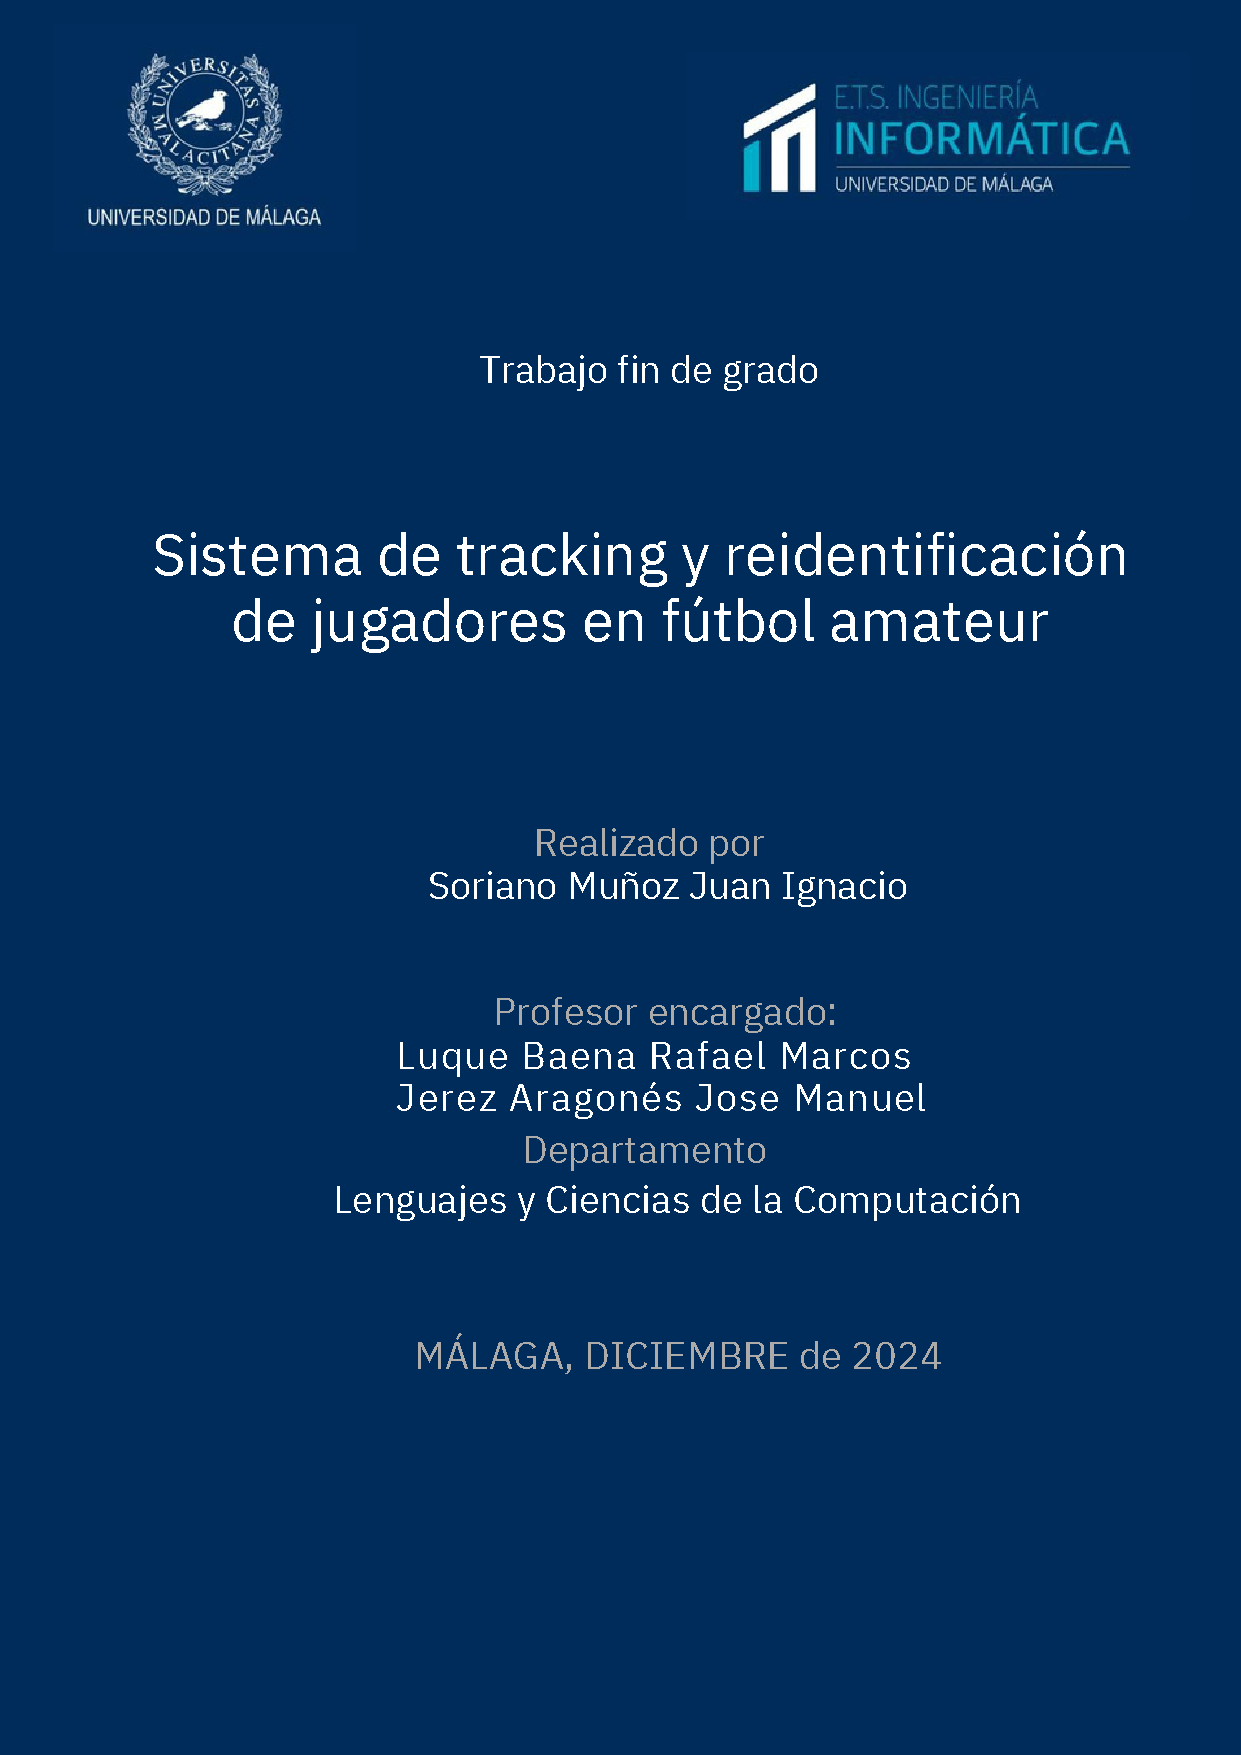
\includepdf[noautoscale=true, width=\paperwidth]{cover.pdf}
	
	%% Title
	\clearpage
	\setcounter{page}{1}
	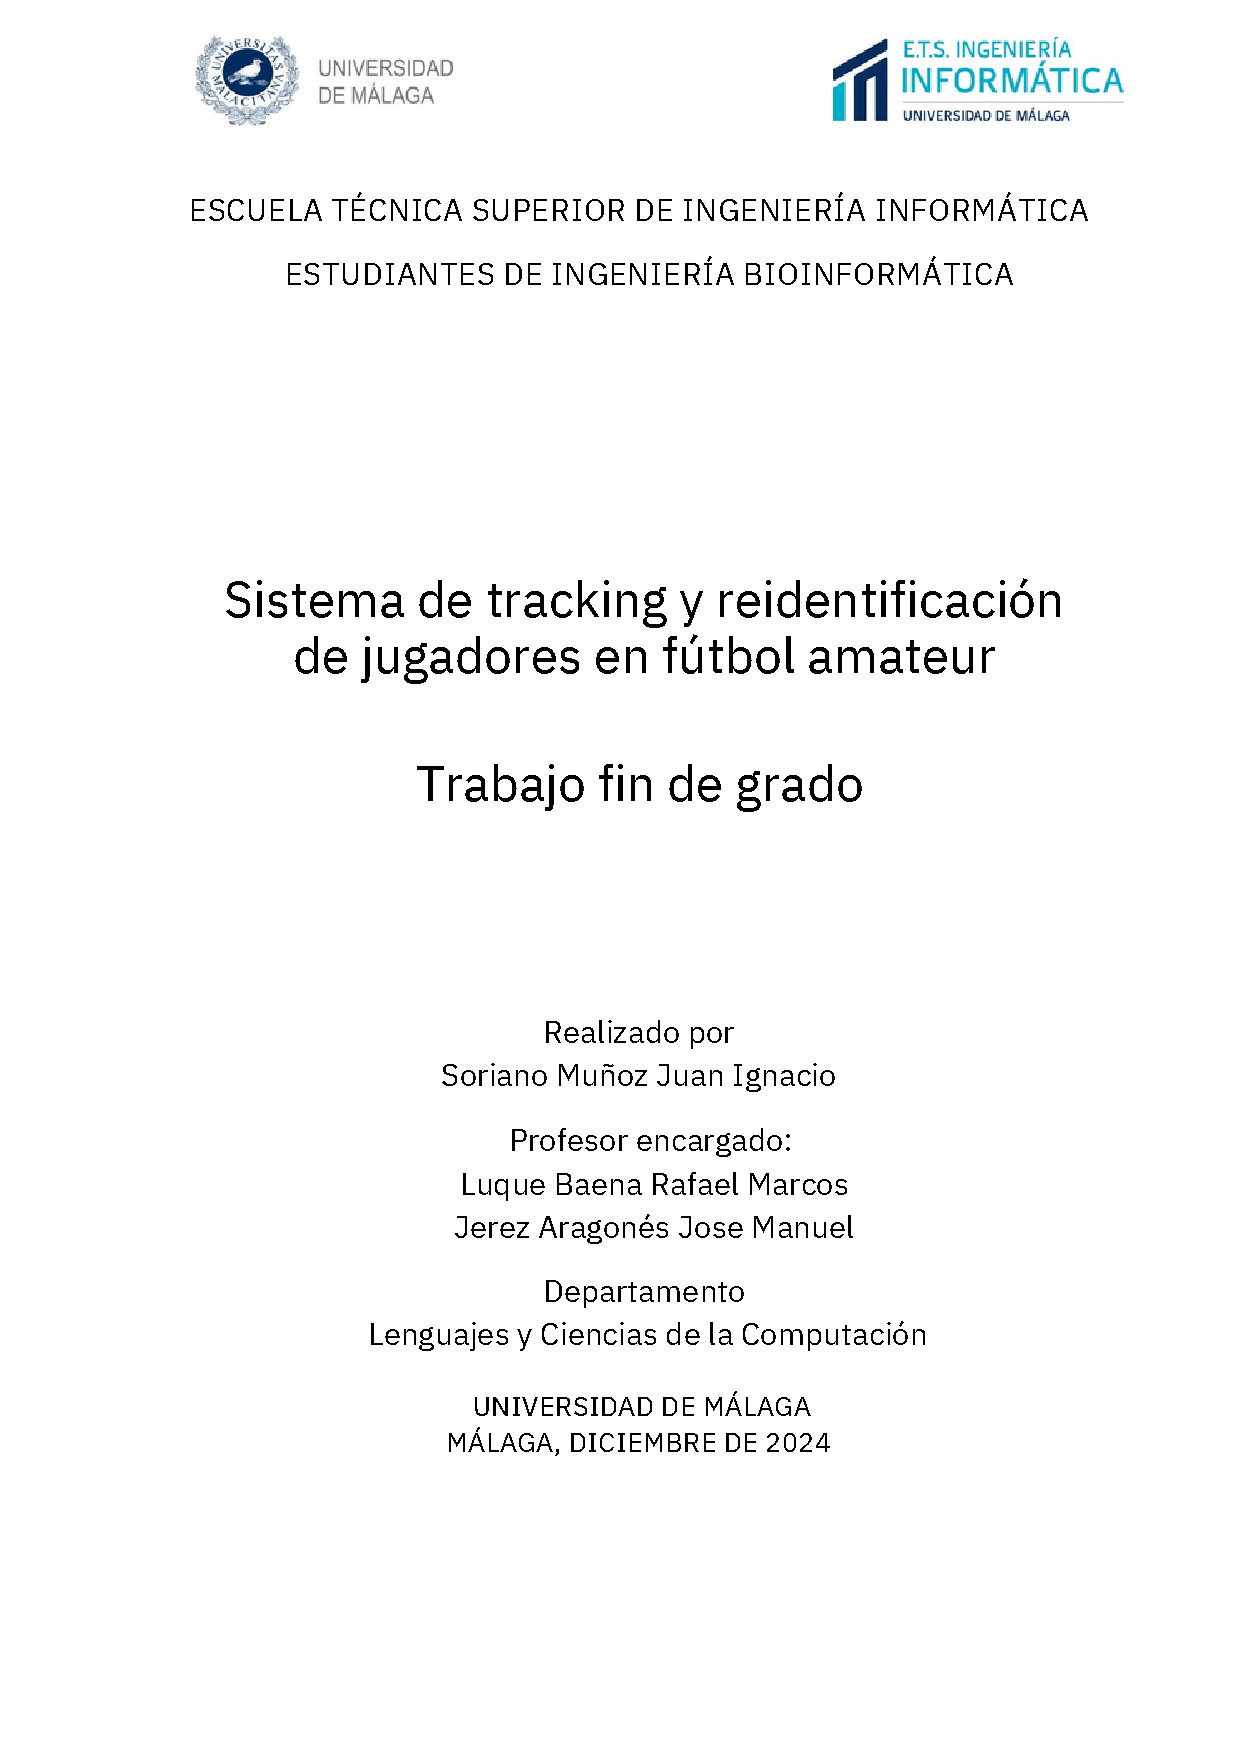
\includepdf[noautoscale=true, width=\paperwidth]{title.pdf}
	
	%%%%%%%%%%%%%%%%%%%%%%%%%%%%%%%%%%%%%%%%%%%%%%%%%%%%%%%%%%%%%%%%%%%%%%%%%%%
	
	% Índice automático
	\tableofcontents
	\newpage
	
	% Sections
	
		% Sections
	\section{Introducción}
	
	\section{Diario de avances}
	
	\subsection{Semana 3-16 de marzo)}
	
	Por ahora lo que llevamos es un dataset hecho en roboflow con un partido de España contra Suiza. Realizamos capturas y dividimos el conjunto en training, validation y test.
	
	Entrené el modelo de YOLO con este dataset revisado y el modelo no supo detectar bien el balón debido a la poca cantidad de imágenes donde se pueda ver bien la bola. El árbitro y los jugadores fueron bien detectados.
	
	Se replanteó el objetivo del TFG. Se focalizará en la reidentificación de jugadores cuando salen fuera de plano y en el desarrollo de una aplicación que permita al usuario decidir si cuando se produce un cambio de identificador, mantenerlo o cambiarlo, creando un dataset revisado.
	
	\subsection{Semana 17-31 de marzo \cite{sun2024gta}}
	
	A la hora de medir resultados como estas gráficas:
	
	\begin{figure}[h]
		\centering
		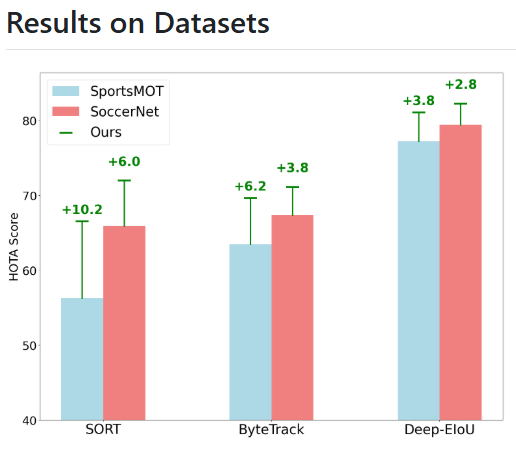
\includegraphics[width=0.8\textwidth]{image/metricasBeta}
		\caption{\textbf{Métricas gta\_link}}
		\label{fig:metricasBeta}
	\end{figure}
	
	Nos centraremos en la medida de los ID's intentando minimizarlos, lo máximo posible, ya que la métrica significa número de ids generados.
	
	\begin{figure}[h]
		\centering
		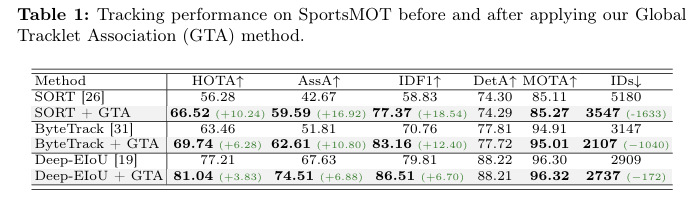
\includegraphics[width=0.8\textwidth]{image/Centrarse}
		\caption{\textbf{Objetivo}}
		\label{fig:Centrarse}
	\end{figure}
	
	Me he puesto a mirar lo que hace exactamente el código del repositorio de gta-link. Y en resumidas cuentas necesitamos un dataset con una pred, ya realizada, como es el caso de SoccerNet. Podemos descargar el dataset con el tracking realizado en los archivos .txt que se encuentran dentro de cada clip.\vspace{0.5cm}
	
	He utilizado las siguientes líneas de comando para realizar la descarga del dataset.
	
	\begin{verbatim}
		from SoccerNet.Downloader import SoccerNetDownloader
		mySoccerNetDownloader = SoccerNetDownloader(LocalDirectory="path/to/SoccerNet")
		mySoccerNetDownloader.downloadDataTask(task="tracking",
		 split=["train","test","challenge"])
	\end{verbatim}
	
	Posteriormente hice unos ajustes en el código para que cogiera los archivos \texttt{gt.txt} para que se tomara como referencia \textbf{--pred\_dir {tracking results directory}}, ya que estos son archivos \textbf{MOT}, que guardan información sobre los \textbf{bounding box} de cada objeto de cada frame, conteniendo información sobre \textbf{frame}, \textbf{id}, \textbf{bb\_left}, \textbf{bb\_top}, \textbf{bb\_width}, \textbf{bb\_height}, \textbf{conf}, \textbf{x}, \textbf{y}, \textbf{z}, en este orden.
	
	Estos son esenciales para que se pueda ejecutar el archivo \texttt{generate\_tracklets.py} para generar los \textbf{tracklets}.
	
	Un \textbf{tracklet} se genera al seguir a un objeto desde su detección en un fotograma hasta el siguiente. En este proceso, el código asocia las detecciones de objetos de cada fotograma con un identificador único (\textbf{ID}) para cada objeto, y los agrupa en una \textbf{"trayectoria"} que sigue ese objeto a lo largo del tiempo.
	
	En el código:
	
	\begin{itemize}
		\item \textbf{Extracción de características:} El código utiliza un modelo de reidentificación de personas (\texttt{FeatureExtractor}) para extraer características visuales de cada objeto detectado en los fotogramas. Esto es útil para seguir objetos entre fotogramas, incluso cuando se producen cambios de apariencia debido a variaciones en la vista o el movimiento.
		\item \textbf{Cálculo de tracklets:} Para cada fotograma, el código agrupa las detecciones de objetos utilizando el identificador único (\texttt{track\_id}). Si un objeto se detecta en un fotograma y luego aparece en otro, se agrega a un tracklet, que es una colección de todas las detecciones del mismo objeto a lo largo de varios fotogramas. Además, se guarda información como el puntaje de la detección y las características extraídas del modelo de reidentificación.
		\item \textbf{Salvado de tracklets:} Al final de cada secuencia de video o serie de fotogramas, los tracklets generados se guardan en un archivo \texttt{pickle} para su posterior uso, permitiendo analizar y trabajar con las trayectorias de los objetos en el futuro.
	\end{itemize}
	
	El programa \texttt{generate\_tracklets.py}, lo que hará será generar unos ficheros \texttt{.pkl} que guardan los datos de las trayectorias de los objetos detectados a lo largo del tiempo. Esto incluye, por ejemplo, las \textbf{detecciones de objetos en cada fotograma}, las \textbf{características extraídas por el modelo de reidentificación}, y los \textbf{identificadores únicos (ID)} asignados a cada objeto (en formato binario).
	
	Una vez que se tenga esos ficheros se realiza una \textbf{refinación de los tracklets} para evitar que se cambien los \textbf{ids con frecuencia}. Mejora los \textbf{tracklets} (trayectorias de objetos) generados por un \textbf{tracker en tareas de seguimiento de múltiples objetos (MOT)}. Utiliza dos componentes principales: el \textbf{Tracklet Splitter}, que divide \textbf{tracklets impuros} (con múltiples identidades) en subtracklets más precisos mediante \textbf{clustering (DBSCAN)}, y el \textbf{Tracklet Connector}, que fusiona \textbf{tracklets fragmentados} que pertenecen al mismo objeto basándose en \textbf{similitudes visuales y restricciones espaciales}. Los resultados refinados se guardan en archivos \texttt{.txt} en formato \textbf{MOT}, listos para su evaluación, visualización o análisis posterior. Este proceso optimiza la \textbf{precisión del seguimiento}, corrigiendo errores como \textbf{cambios de identidad} y \textbf{fragmentaciones}.\vspace{0.5cm}
	
	
	Ahora que tenemos un dataset etiquetado, tendremos que:
	
	\begin{itemize}
		\item \textbf{Encontrar una combinación de hiperparámetros óptima: } Con el objetivo de que el cambio de ids sea el mínimo posible.
		\item \textbf{Desarrollar una aplicación: } Con el objetivo de que avise al usuario sobre los cambios de id en los frames y confirme si está bien cambiado o debería conservarse el anterior.
	\end{itemize}
	
	\subsection{Semana 31-6 de abril)}
	
	En estas semanas hemos estado invirtiendo tiempo en las siguientes cosas. En un principio lo que teníamos era un dataset preparado con los ficheros ground truth fruto de un tracker usado (como DeepEIoU). Pero dado un vídeo, no podíamos aplicar los programas de gta-link, por lo que teníamos que conseguir los ficheros MOT de alguna manera. 
	
	Había dos opciones. La primera aplicar un tracker y la segunda aplicar un modelo de YOLO.
	
	Para la primera opción busqué en varios repositorios, que trataran con trackers, principalmente DeepEIoU, que es el tracker con el mejor rendimiento según las estadísticas de paperscode \cite{sportsmot_paperswithcode}.
	
	\begin{figure}[h]
		\centering
		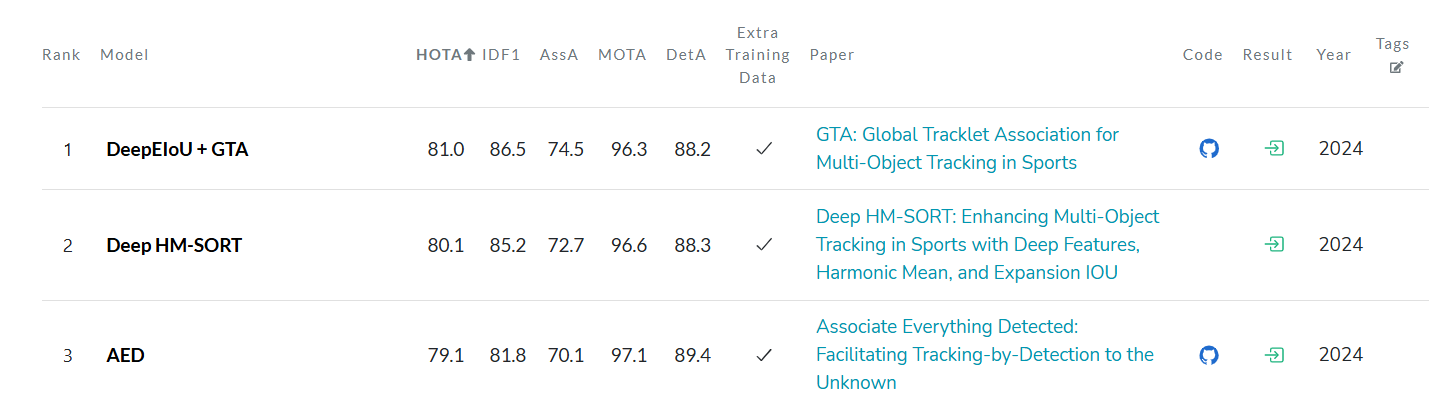
\includegraphics[width=0.8\textwidth]{image/deepEIoU}
		\caption{\textbf{Métricas DeepEIoU}}
		\label{fig:deepEIoU}
	\end{figure} 
	
	Tras encontrar un repositorio que trataba en específico con este \cite{huang2024iterative}. Tuve que modificar código para que utilizara cpu, ya que estaba configurado para gpu de nvidia. Los paquetes no se me instalaban correctamente. Los inputs que utilizaba para los programas eran ficheros tipo .npy.
	
	Dado que me estaba dando muchos problemas, después de dos días decidí que la mejor solución era utilizar un modelo de YOLO. Empecé utilizando un modelo de YOLO estandar capaz de detectar personas. El inconveniente de esto es que el video, estaba grabado desde un ángulo muy bajo, por lo que el modelo detectara las personas de las gradas y esto, a la larga, es un problema. 
	
	Entonces para resolver esto había dos opciones. La primera era realizar una segmentación del campo y la segunda entrenar un modelo de YOLO específico para jugadores. La segmentación del campo es demasiado costosa, porque no hay nada automatizado y sería segmentar infinidad de frames. Además de que es específica para un partido de fútbol en un ángulo en específico.Por lo tanto, la mejor opción para mi gusto es entrenar un modelo de YOLO con un dataset, por ahora, específico del partido de balonmano que me proporcionó mi tutor Jose Manuel Jerez. El dataset lo hice creando un programa utilizando las librerias de opencv (cv2) que extraía frames cada 20 segundos que transcurría de vídeo. Los 20 segundos previenen levemente más overfitting del que ocurre por tener frames del mismo partido. 
	
	Esta opción me permite etiquetar poco, ya que Roboflow tiene una herramienta de etiquetado automático una vez se han etiquetado unas cuantas imágenes, por lo que simplemente tuve que corregir aquellas imágenes con un mal etiquetado.
	
	Tras tener el dataset etiquetado le añadí algunas augmentations. 
	
	A la hora de entrenar el modelo lo hice con 25 epochs. Tardó hora y media en entrenarse.
	
	Apliqué los programas del repositorio de gta-link y los resultados del trackeo son muy buenos, pero la ReID no tiene nada que ver con los resultados tan consistentes del dataset de SoccerNet debido a que la grabación no es profesional.
	
	Aun así tras 23 intentos observe que los parámetros que daban mejores resultados eran los siguientes: --use\_split --min\_len 100 --eps 0.8 --min\_samples 10 --max\_k 4 --use\_connect --spatial\_factor 1.0 --merge\_dist\_thres 0.7   
	
	Recientemente le he añadido frames del partido de fútbol 7 al dataset de roboflow. Y he creado un nuevo modelo de YOLO entrenado exclusivamente con ese dataset.
	
	Los objetivos para la próxima semana:
	
	\begin{itemize}
		\item \textbf{Buscar como aplicar un tracker:} Después de aplicar un trackeo con YOLO, sería necesario aplicar DeepEIoU. Investigar si aplicar un doble gta-link puede funcionar para refinar los tracklets todavía más.
		\item \textbf{Seguir desarrollando la aplicación: } Con el objetivo de que avise al usuario sobre los cambios de id en los frames y confirme si está bien cambiado o debería conservarse el anterior. Ya tengo un programa prueba\_revision\_ReID.py, que funciona como prototipo, pero falta desarrollarlo mucho.
	\end{itemize}
	
	\subsection{Semana 7-13 de abril)}
	
	Al final el proceso de usar el tracker es obligatorio, ya que los objetos son detectados por YOLO, pero luego los ids son colocados por el tracker, y de ahí saldrán ficheros tipo MOT. Entonces tras aplicar YOLO para tener ficheros con la info de los bounding box sobre los jugadores intentaremos aplicarle un tracker y de ahí  un modelo de ReID, para posteriormente utilizar gta.
	
	Secuencia de trabajo: YOLO + DeepEIoU + GTA
	
	\subsection{Semana 7-13 de abril)}
	
	Planteé una estructura oficial de lo que llevo hecho para que sea más formal y dar contexto e información sobre todo lo que rodea las prácticas y el proyecto de TFG.
	
	\section{Motivación y Contexto}
	
	\subsection{¿Por qué es importante el análisis en fútbol amateur?}
	
	El análisis de rendimiento, la estadística avanzada y el seguimiento de jugadores han revolucionado el fútbol profesional. Sin embargo, en el fútbol amateur estas tecnologías todavía son muy poco accesibles.
	Poder aplicar técnicas de tracking y análisis en estos niveles permitiría:
	\begin{itemize}
		\item \textbf{Mejorar el entrenamiento de jugadores jóvenes.}
		\item \textbf{Facilitar la toma de decisiones a entrenadores y clubes pequeños.}
		\item \textbf{Promover el desarrollo del talento de forma más justa y basada en datos.}
	\end{itemize}
	
	\subsection{¿Qué problema hay actualmente?}
	
	La causa del primer problema que encontramos es la deficiencia en las infraestructuras tecnológicas para la práctica del fútbol amateur; el hecho de no disponer de sistemas avanzados que implementan las cámaras múltiples o los sensores del fútbol en el sector profesional, por el alto coste que implicaría el uso de las soluciones comerciales de tracking (GPS, cámaras VICON, sistemas ópticos, etc.) y la escasez de datos de movimiento y rendimiento que sufren las categorías base y amateur.
	
	\section{Objetivos}
	
	Este trabajo tiene como fin principal reducir esta brecha poniendo a punto un flujo del trabajo modular y eficiente que permita trasladar al ámbito amateur la tecnología de vanguardia en visión por computador. Para ello, se combinan modelos de detección de objetos (YOLOX y YOLOv10) con algoritmos de seguimiento multiobjeto (DeepEIoU) y técnicas de reidentificación de personas (ReID) mediante el modelo OSNet. Al mismo tiempo también se utiliza un sistema de refining posterior (GTA-Link) que mejora la calidad de las trayectorias generadas y corrige inconsistencias típicas del seguimiento, como la fragmentación de identidades.
	
	Dado que el flujo de trabajo es más amplio que la obtención de las salidas visuales y estructuradas (vídeos anotados Archivos MOT) se busca también la evaluación de forma cuantitativa del rendimiento de los modelos de ReID utilizados, de este modo se habilita un entorno experimental donde comparar diferentes aportaciones de reidentificación a través de métricas bien definidas como mAP Rank-k lo que permite reforzar el análisis y la elección de los modelos más adecuados en los escenarios bajo el análisis de vídeo.
	
	Los objetivos específicos del proyecto son los siguientes:
	
	\begin{itemize}
		\item Diseñar y desarrollar un flujo de trabajo completo que permita evaluar modelos de reidentificación de manera objetiva y repetible.
		\item Generar vídeos anotados y sus correspondientes archivos MOT en formato \texttt{.txt}, que representen con fidelidad las trayectorias e identidades de los jugadores durante un partido.
		\item Implementar un sistema que mantenga la coherencia de los IDs asignados a los jugadores incluso ante oclusiones, desapariciones temporales o entradas/salidas de la escena.
		\item Establecer una metodología de evaluación que permita comparar distintos modelos de ReID mediante métricas como mAP y Rank-k sobre conjuntos de datos reales.
		\item Fomentar la reutilización y ampliación del flujo de trabajo en otros entornos deportivos no profesionales, facilitando su adopción en el fútbol base o amateur.
	\end{itemize}

	
	\section{Estado del sector}
	
	El análisis de rendimiento en el fútbol ha experimentado una transformación significativa en las últimas décadas, impulsada por avances tecnológicos que permiten una recopilación y procesamiento de datos cada vez más precisos y en tiempo real. Sin embargo, existe una marcada diferencia entre las herramientas utilizadas en el ámbito profesional y las accesibles para equipos amateurs.
	
	\subsection{Soluciones en el Ámbito Profesional}
	
	En el fútbol profesional, sistemas como TRACAB se han consolidado como referentes en el seguimiento y análisis de jugadores. TRACAB es un sistema de seguimiento óptico que utiliza cámaras y algoritmos de visión por computadora para rastrear en tiempo real la posición de todos los jugadores y el balón en el campo. Este sistema ha sido implementado en ligas de élite como la Premier League, La Liga y la Bundesliga, y está certificado por la FIFA para programas de seguimiento electrónico de rendimiento (EPTS). "https://tracab.com/products/tracab-technologies/?utm\_source=chatgpt.com"
	
	\begin{figure}[H]
		\centering
		\begin{minipage}{0.45\textwidth} % Controla el ancho de la imagen
			\centering
			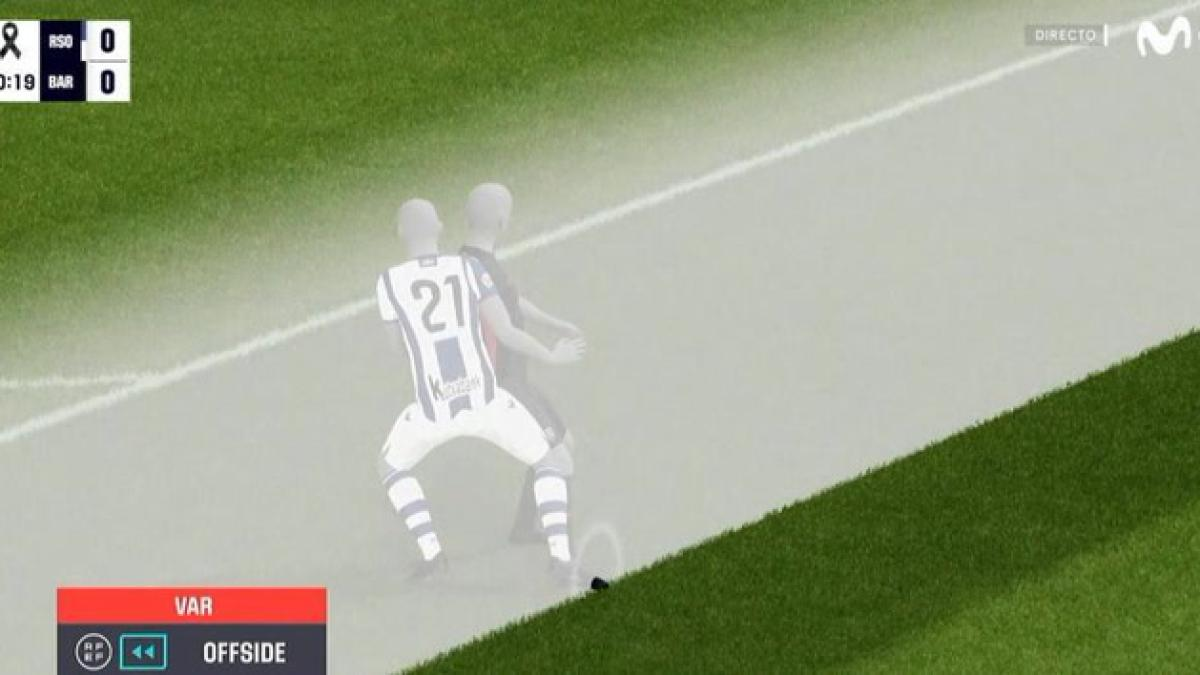
\includegraphics[width=\textwidth]{image/tracab}
			\label{tracab}
		\end{minipage}
		\hfill
		\begin{minipage}{0.45\textwidth} % Controla el ancho de la imagen
			\centering
			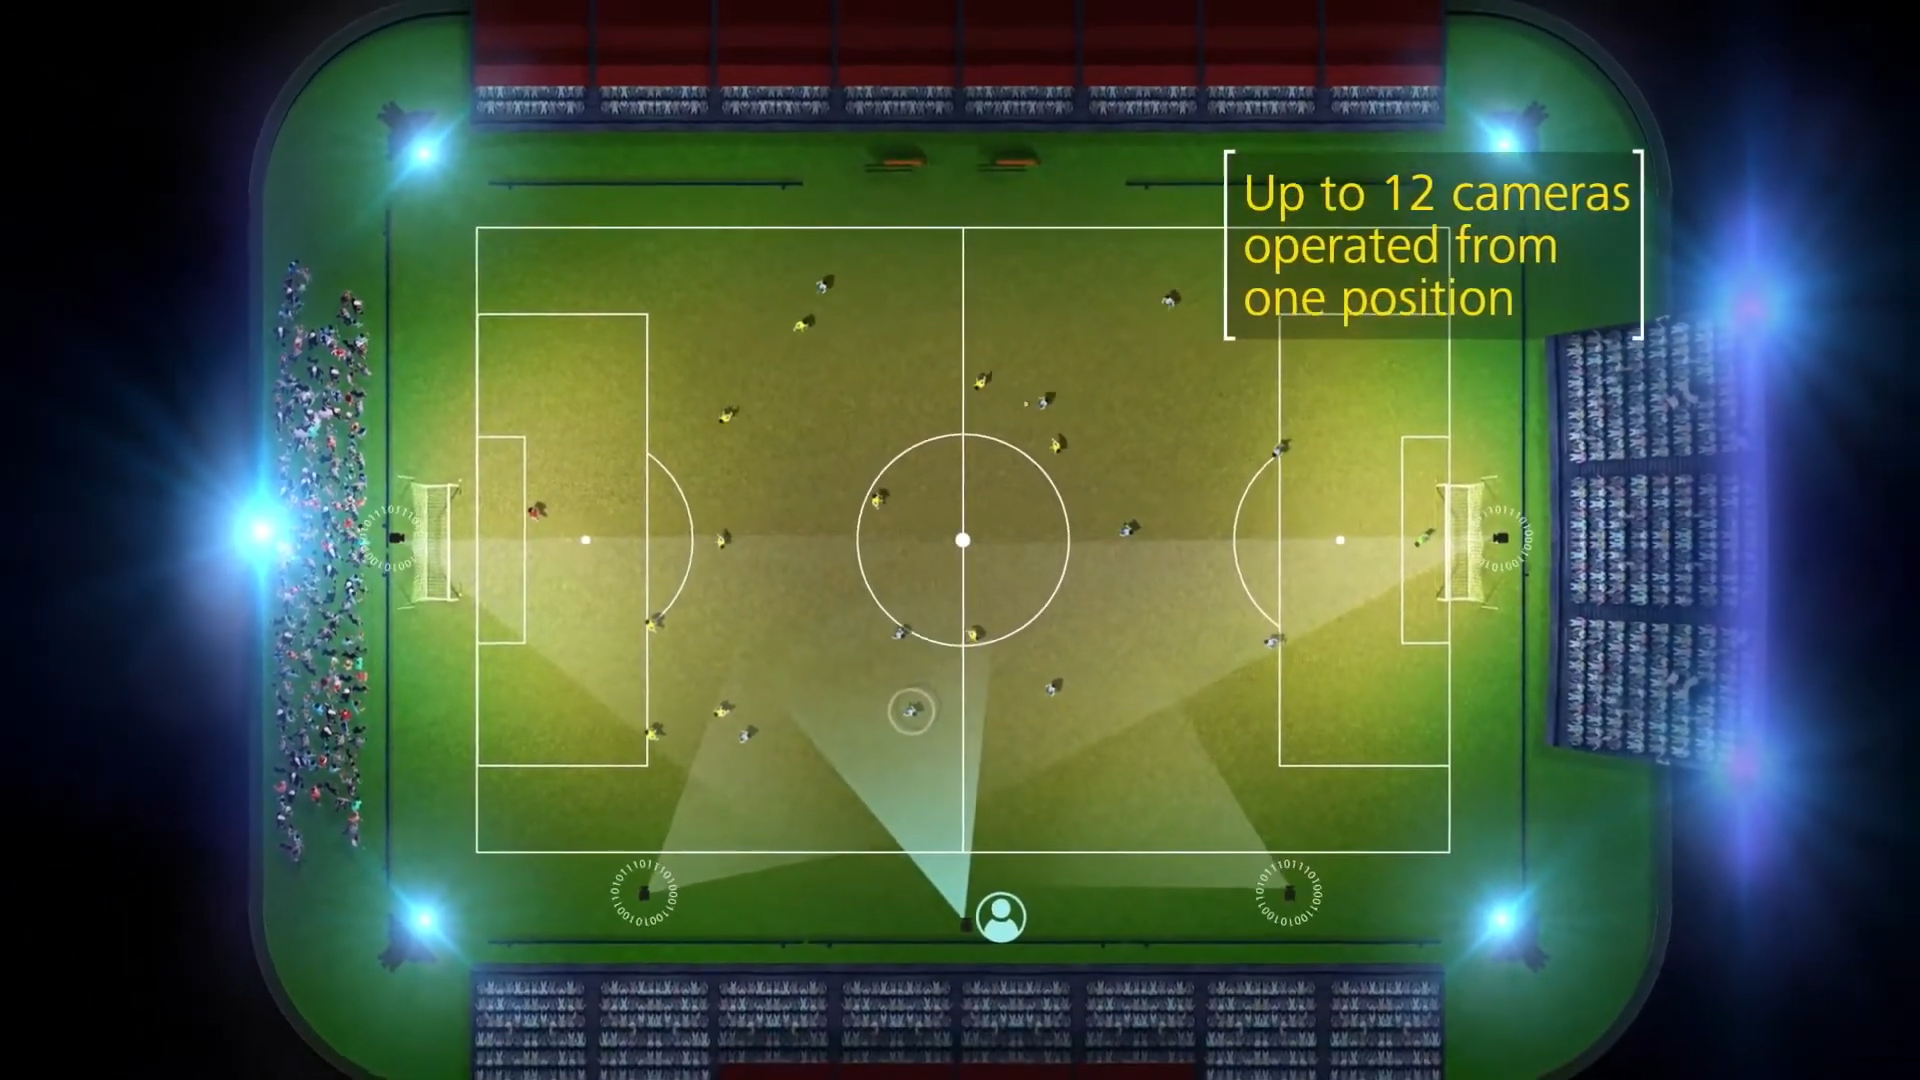
\includegraphics[width=\textwidth]{image/tracab2}
			\label{tracab2}
		\end{minipage}
		\caption{\textbf{Tracab}}
	\end{figure}
	
	
	\subsection{Herramientas Disponibles para el Fútbol Amateur}
	
	En contraste, el fútbol amateur ha comenzado a adoptar herramientas más asequibles y adaptadas a sus necesidades y recursos. Una de las más destacadas es LongoMatch, un software de análisis de vídeo que permite a entrenadores y analistas etiquetar eventos, crear estadísticas y generar informes tácticos a partir de grabaciones de partidos.
	
	\begin{figure}[h]
		\centering
		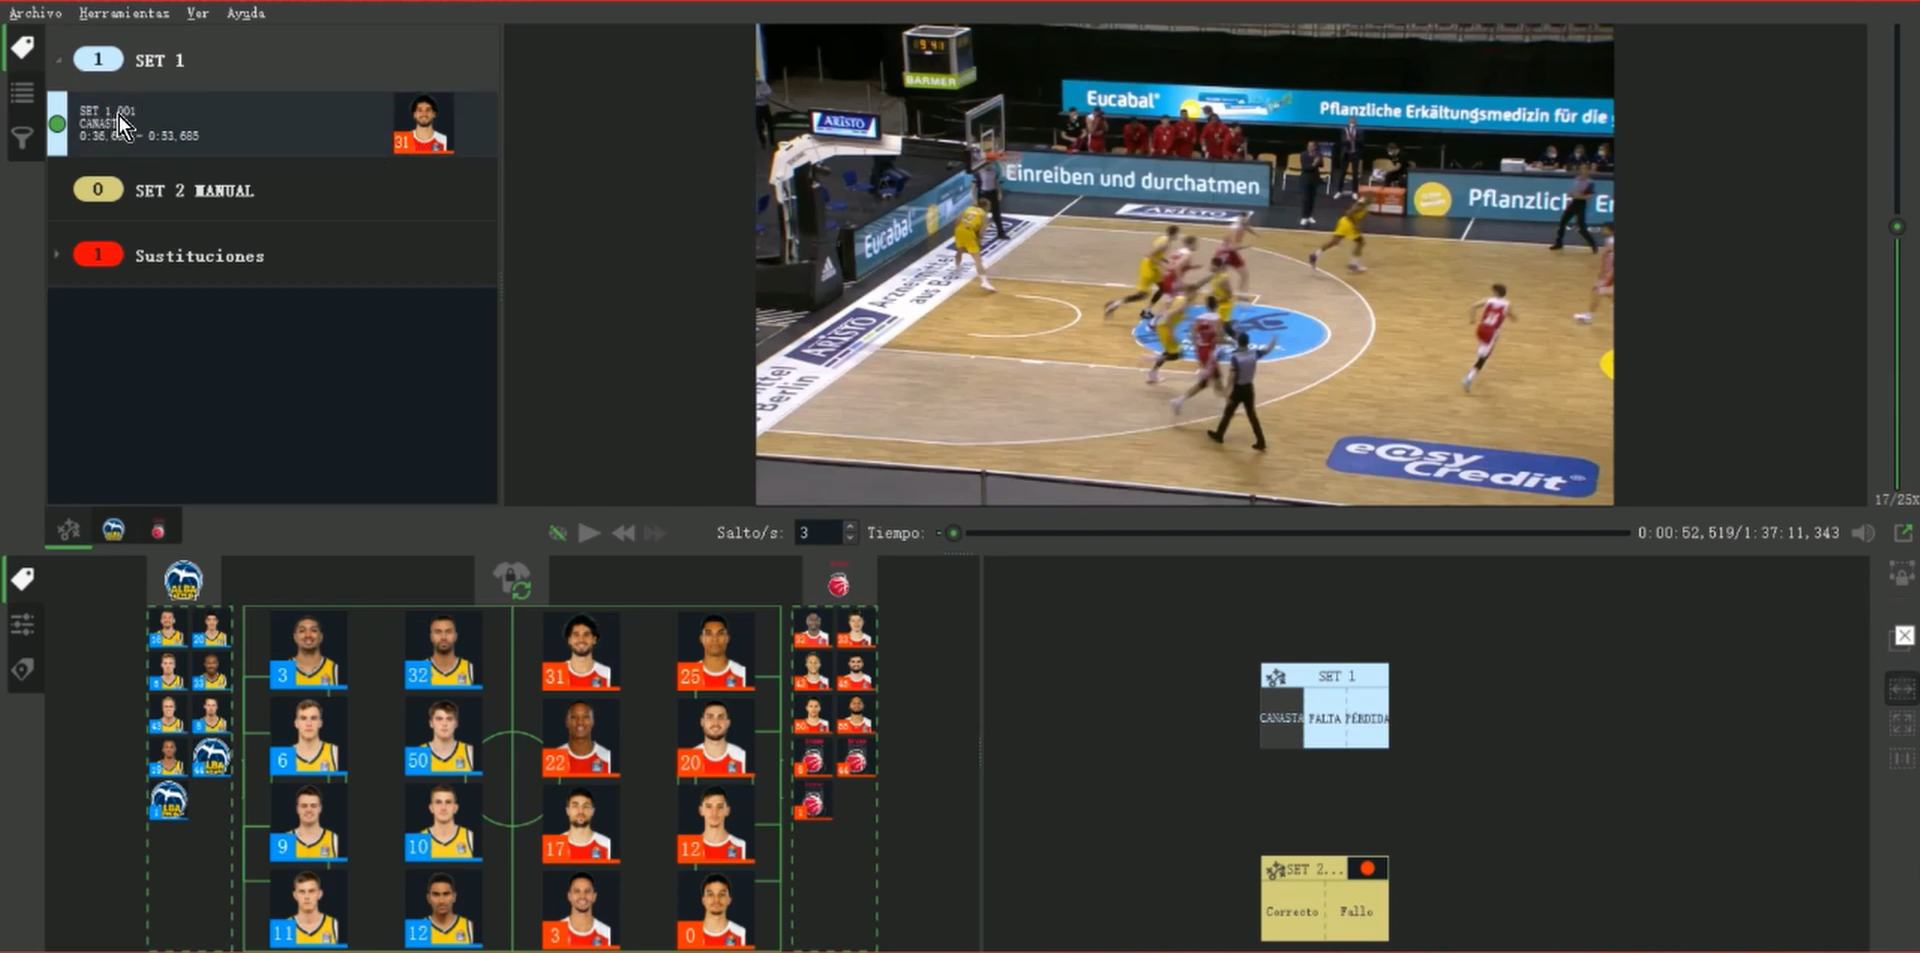
\includegraphics[width=0.8\textwidth]{image/longomatch}
		\caption{\textbf{Interfaz de Longomatch}}
		\label{fig:longomatch}
	\end{figure} 
	
	LongoMatch ofrece "https://longomatch.com/en/":
	\begin{itemize}
		\item	Análisis en tiempo real y post-partido con soporte para múltiples cámaras.

	
		\item Personalización de paneles de análisis según las necesidades del equipo.
	
		\item Exportación de datos y vídeos para compartir con jugadores y cuerpo técnico.
	
		\item Compatibilidad con diversas plataformas y dispositivos móviles.
	\end{itemize}
	
	Además, herramientas como PIX4TEAM 2 han emergido para automatizar la grabación de partidos sin necesidad de un operador de cámara, facilitando la recopilación de material para análisis en equipos con recursos limitados. "https://shop.movensee.com/es/content/31-pix4team-camara-automatica-para-los-deportes-colectivos"
	
	\subsection{Limitaciones}
	
	\begin{center}
		\begin{tabular}{|p{6.5cm}|p{6.5cm}|}
			\hline
			\textbf{Limitaciones del sector amateur} & \textbf{Aportaciones del presente proyecto} \\
			\hline
			Los sistemas comerciales como Second Spectrum o STATS SportVU requieren múltiples cámaras y hardware costoso. &
			Se utiliza vídeo monocámara accesible y fácil de capturar con dispositivos comunes. \\
			\hline
			Los trackers convencionales pierden frecuentemente la identidad del jugador en escenas con oclusiones o cambios de plano. &
			Se implementa un módulo de re-identificación (ReID) basado en TorchReID y OSNet para mantener la identidad a lo largo del partido. \\
			\hline
			No existen herramientas que generen anotaciones automáticas de forma sencilla a partir del vídeo. &
			Se desarrolla un flujo de trabajo que genera archivos de anotaciones (formato MOT) automáticamente a partir del vídeo de entrada. \\
			\hline
			Los modelos existentes están entrenados en entornos profesionales, con condiciones muy diferentes al fútbol amateur. &
			Los modelos utilizados en este proyecto han sido entrenados y validados específicamente sobre partidos de fútbol amateur. \\
			\hline
			Las soluciones actuales no están diseñadas para clubes pequeños: requieren licencias, suscripciones o personal técnico. &
			Se busca una solución reproducible, ligera y gratuita basada en herramientas \textit{open-source}, accesible a cualquier usuario técnico. \\
			\hline
		\end{tabular}
	\end{center}
	
	\section{Tecnologías empleadas}
	
	Este proyecto ha hecho uso de diversas tecnologías de software y frameworks de inteligencia artificial que permiten implementar un sistema de tracking con detección, seguimiento y reidentificación de jugadores en partidos de fútbol amateur. A continuación, se detallan las principales herramientas y recursos utilizados.
	
	\subsection{Programación}
	
	Para el desarrollo del sistema se ha utilizado el lenguaje de programación Python, por su gran ecosistema de librerías para visión por computadora y deep learning. El flujo de trabajo se ha dividido en diferentes etapas, desarrolladas principalmente en entornos Jupyter Notebook y scripts de Python:
	
	\begin{itemize}
		\item \textbf{Jupyter Notebook:} Se utilizó para entrenar el modelo de detección de objetos YOLO, aprovechando la facilidad para experimentar de forma interactiva con parámetros y visualizar resultados.
		\item \textbf{Python (scripts):} Fue empleado para el entrenamiento del modelo de re-identificación (ReID), así como para aplicar todos los modelos en el flujo final de inferencia y generación de vídeos etiquetados con las predicciones.
	\end{itemize}
	
	\subsection{Gestión de datos y flujo de trabajo}
	
	\textbf{Roboflow} ha sido una herramienta fundamental para gestionar el dataset de entrenamiento del detector YOLO. Roboflow permite subir imágenes, etiquetarlas, realizar aumentos de datos automáticamente y exportar el dataset en el formato deseado (en nuestro caso, YOLOv8).
	
	\textbf{GitHub} ha sido el sistema elegido para el control de versiones y colaboración. Se ha utilizado para organizar y almacenar los diferentes módulos del proyecto, así como mantener un historial ordenado de los avances y pruebas realizadas durante el desarrollo de las prácticas(TFG).
	
	\subsection{Modelos utilizados}
	
	\textbf{YOLO (You Only Look Once)} ha sido el modelo principal utilizado para la detección de jugadores. Su arquitectura permite realizar detección en tiempo real, con una alta precisión y bajo coste computacional. Se entrenó una versión ligera del modelo con imágenes de fútbol amateur obtenidas del dataset gestionado en Roboflow.
	
	\textbf{DeepEIoU} fue el algoritmo de tracking utilizado para asociar detecciones entre frames y mantener la identidad de cada jugador. DeepEIoU combina estrategias geométricas (IoU) y de apariencia (cuando se usa ReID), lo que mejora la robustez frente a oclusiones y cambios de plano.
	
	Este modelo ha sido clave para generar archivos de anotación con los ID temporales de los jugadores a lo largo del vídeo, y servir como base para el post-procesamiento posterior mediante GTA-Link.
	
	\textbf{TorchReID} se ha usado como framework para entrenar el modelo de re-identificación. Se utilizó el modelo \textit{osnet\_x1\_0}, que fue ajustado sobre imágenes recortadas de jugadores, organizadas en carpetas según su identidad. Este modelo se utilizó posteriormente para mejorar el seguimiento, reduciendo los cambios de identidad.
	
	
	
	\section{Módulo de detección (YOLO)}
	https://arxiv.org/abs/1506.02640
	
	\subsection{Arquitectura YOLO}
	
	YOLO (You Only Look Once) es una arquitectura de detección de objetos en imágenes y vídeos que ha destacado por su velocidad y precisión. La arquitectura original de YOLO, según la propuesta en el artículo de Redmon et al. (2016)\footnote{Redmon, J., Divvala, S., Girshick, R.,  Farhadi, A. (2016). You Only Look Once: Unified, Real-Time Object Detection. arXiv preprint arXiv:1506.02640.}, se inspira parcialmente en GoogleNet y está compuesta por 24 capas convolucionales, cuatro capas de agrupamiento máximo (max pooling) y dos capas totalmente conectadas al final.
	
	Antes de procesarse, la imagen de entrada es redimensionada a un tamaño fijo de 448x448 píxeles. El flujo interno de la red emplea convoluciones de tipo 1x1 que tienen como función principal reducir el número de canales de activación intermedios sin afectar a la información espacial. Posteriormente, se aplican convoluciones de 3x3 para capturar patrones locales más complejos. Cada una de estas capas es seguida por una función de activación ReLU, que introduce no linealidad al modelo, excepto en la capa de salida, donde se emplea una función de activación lineal.
	
	Además, para mejorar la estabilidad del entrenamiento y evitar el sobreajuste, se aplican técnicas como la normalización por lotes (Batch Normalization) y el abandono (Dropout). Estas estrategias permiten que el modelo generalice mejor ante nuevos datos y se mantenga robusto frente a variaciones del entorno.
	
	Esta arquitectura permite que YOLO realice detección de múltiples objetos en una sola pasada sobre la imagen (de ahí su nombre), lo que lo convierte en un modelo extremadamente eficiente para tareas en tiempo real.
	
	\subsection{¿Cómo funciona la detección de objetos con YOLO?}
	
	Una vez entendida la arquitectura interna de YOLO, es importante comprender cómo se lleva a cabo el proceso de detección de objetos. Para ello, se puede imaginar el caso práctico de una aplicación que detecta jugadores y balones de fútbol a partir de una imagen de vídeo.
	
	\begin{figure}[H]
		\centering
		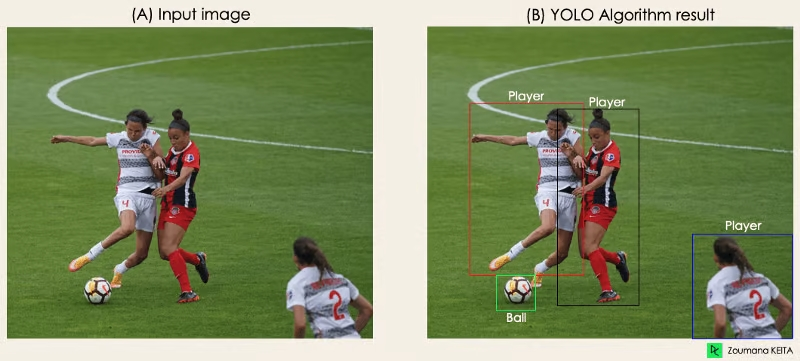
\includegraphics[width=0.8\textwidth]{image/yolodec1}
		\caption{\textbf{YOLO Detection. First Step}}
		\label{fig:YOLO Detection. First Step}
	\end{figure}
	
	El algoritmo de detección en YOLO se basa en cuatro pilares fundamentales: la división en cuadrículas, la regresión de cajas delimitadoras (bounding boxes), el cálculo del coeficiente de intersección sobre unión (IoU), y la supresión no máxima (NMS).
	
	\begin{enumerate}
		\item \textbf{División en cuadrículas (bloques residuales):} La imagen de entrada se divide en una cuadrícula de tamaño $N\times N$, donde cada celda es responsable de detectar los objetos que contiene. Cada celda predice una clase y una probabilidad asociada, además de parámetros que definen la caja delimitadora. 
		
		\begin{figure}[H]
			\centering
			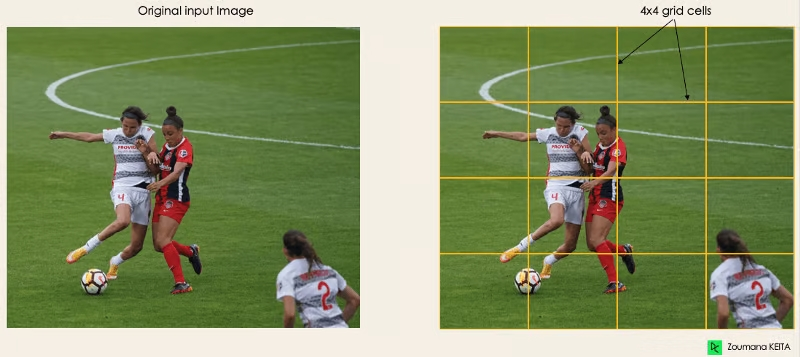
\includegraphics[width=0.8\textwidth]{image/yolodec2}
			\caption{\textbf{YOLO Detection. Second Step}}
			\label{fig:YOLO Detection. Second Step}
		\end{figure}
		
		
		\item \textbf{Regresión de cajas delimitadoras:} Cada celda predice varias cajas en el formato $Y = [p_c, b_x, b_y, b_h, b_w, c_1, c_2, \dots, c_n]$, donde:
		\begin{itemize}
			\item $p_c$ es la probabilidad de que la celda contenga un objeto.
			\begin{figure}[H]
				\centering
				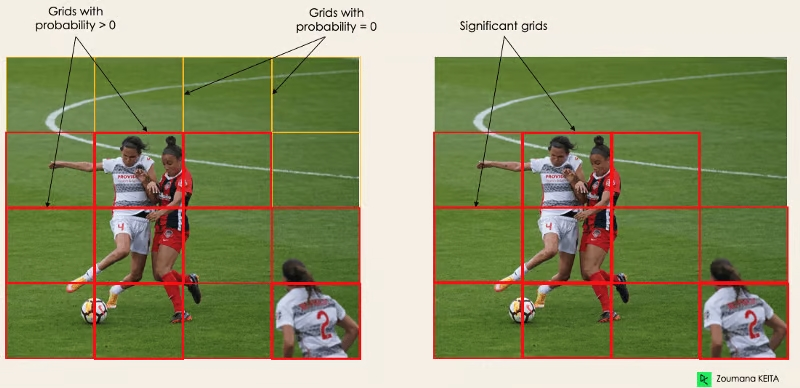
\includegraphics[width=0.8\textwidth]{image/yolodec3}
				\caption{\textbf{YOLO Detection. Third Step}}
				\label{fig:YOLO Detection. Third Step}
			\end{figure}
			\item $b_x$, $b_y$ son las coordenadas del centro de la caja respecto a la celda.
			\item $b_h$, $b_w$ son la altura y la anchura de la caja.
			\item $c_1, c_2, \dots$ son las probabilidades de pertenencia a cada clase (jugador, balón, etc.).
		\end{itemize}
		
		\begin{figure}[H]
			\centering
			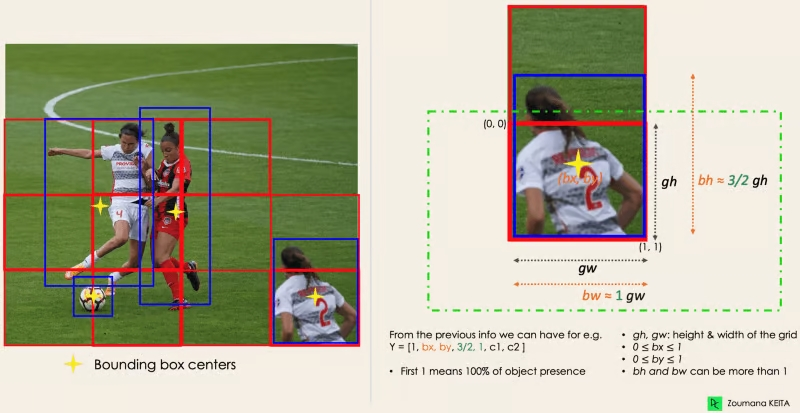
\includegraphics[width=0.8\textwidth]{image/yolodec4}
			\caption{\textbf{YOLO Detection. Fourth Step}}
			\label{fig:YOLO Detection. Fourth Step}
		\end{figure}
		
		
		
		
		\item \textbf{Intersección sobre Unión (IoU):} Para cada predicción, YOLO calcula el solapamiento entre la caja predicha y las cajas reales (ground truth). El valor del IoU (entre 0 y 1) permite descartar predicciones de baja calidad. Sólo aquellas con un IoU superior a un umbral son tenidas en cuenta.
		
		\begin{figure}[H]
			\centering
			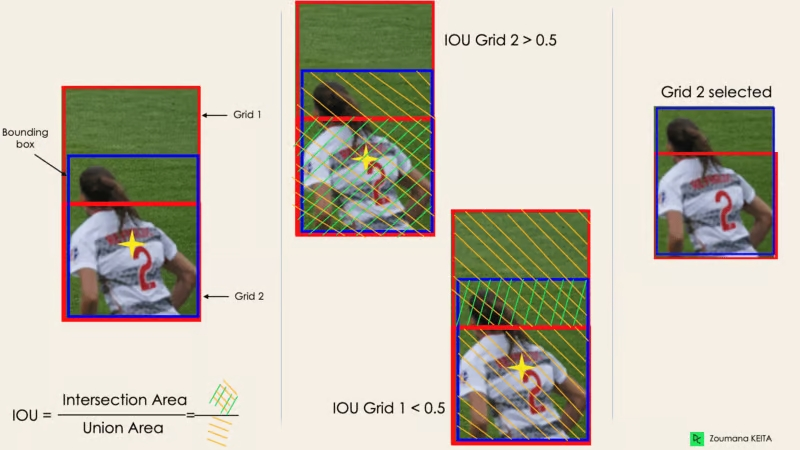
\includegraphics[width=0.8\textwidth]{image/yolodec5}
			\caption{\textbf{YOLO Detection. Fifth Step}}
			\label{fig:YOLO Detection. Fifth Step}
		\end{figure}
		
		
		\item \textbf{Supresión No Máxima (NMS):} Cuando varias cajas se solapan con valores altos de IoU, el algoritmo aplica NMS para conservar sólo la de mayor probabilidad, eliminando duplicados y reduciendo el ruido en las predicciones.
	\end{enumerate}
	
	Este proceso completo permite que, en un único paso y de forma muy eficiente, YOLO identifique múltiples objetos en una imagen, indicando su clase y ubicación precisa. Esta capacidad lo convierte en una herramienta especialmente útil en el análisis de vídeo deportivo, donde se requiere detectar varios jugadores en escenas rápidas y dinámicas.
	"https://www.datacamp.com/blog/yolo-object-detection-explained"
	
	
	\section{Módulo de tracking + Gestión de IDs}
	
	
	\subsection{Módulo de tracking}
	En el contexto de la detección de objetos en vídeo, como la realizada por modelos como YOLO, cada fotograma es procesado de forma independiente. Esto significa que, aunque el detector puede identificar y localizar objetos en cada imagen, no mantiene información sobre la identidad de estos objetos a lo largo del tiempo. Por ejemplo, no puede determinar si el jugador detectado en el fotograma 1 es el mismo que en el fotograma 2.
	
	Para abordar esta limitación, se emplean algoritmos de seguimiento de objetos (trackers) que asocian las detecciones entre fotogramas consecutivos, permitiendo así mantener la identidad de cada objeto a lo largo del tiempo. Estos trackers asignan un identificador único a cada objeto y actualizan su posición en cada nuevo fotograma, incluso en presencia de oclusiones o cambios de apariencia.
	
	\begin{figure}[H]
		\centering
		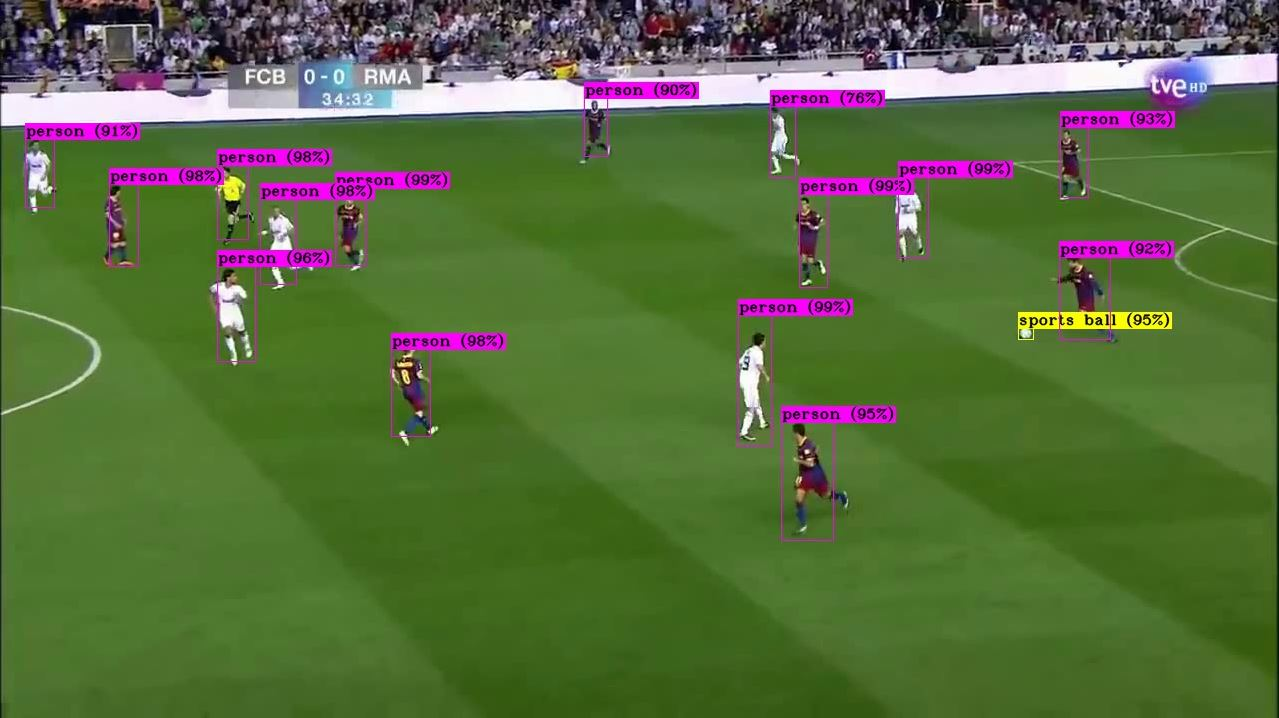
\includegraphics[width=0.8\textwidth]{image/tracking_id}
		\caption{\textbf{Tracking}}
		\label{tracking_id}
	\end{figure}
	
	Un ejemplo destacado de este enfoque es el algoritmo Deep SORT (Simple Online and Realtime Tracking with a Deep Association Metric), que combina información de movimiento y apariencia para asociar detecciones entre fotogramas. Deep SORT utiliza un filtro de Kalman para predecir la posición futura de los objetos y un descriptor de apariencia basado en redes neuronales profundas para comparar similitudes visuales entre detecciones. La asociación entre detecciones y trayectorias se realiza mediante el algoritmo húngaro, que minimiza el coste total de asociación considerando tanto la distancia de movimiento como la similitud de apariencia.
	"https://doi.org/10.1109/ICIP.2017.8296962"
	
	\subsection{Gestión de IDs}
	
	"https://paperswithcode.com/task/person-re-identification"
	
	La Re-identificación de Personas es una tarea de visión por computadora cuyo objetivo es asociar la identidad de una persona a través de diferentes cámaras o ubicaciones en una secuencia de vídeo o imágenes. Esto lo hacemos mediante modelos de ReID. 
	
	Los modelos de reidentificación de personas (ReID), tal y como OSNet o ResNet, están orientados a transformar las imágenes de las personas en vectores numéricos, generalmente conocidos como \textit{embeddings} que resumen visualmente el aspecto de cada uno de los bebés. Para ello, comienzan por la imagen de entrada, que normalmente tiene 3 canales (RGB: rojo, verde y azul). Con la red convolucional, esta imagen es tratada por varios filtros que producen canales intermedios de activación. Dichos canales pueden ir desde docenas de ellos hasta miles de ellas, y entonces dejan de representar colores básicos y empiezan a representar patrones visuales más complejos: texturas de la ropa, formas del cuerpo, tipo de vestimenta o incluso composiciones más estrictas de rasgos visuales. Cada canal puede ser entendido como un detector especializado en la obtención de cierta característica, y en conjunto ellos forman un mapa de activación tridimensional. Al final de la red, dichos mapas son reducidos por pooling global y son luego aplanados para las embeddings finales, que son un vector de gran dimensión (ejemplo 512 números), donde cada número codifica una sección abstracta del aspecto visual del jugador. Este vector no representa un ID explícito sino una posición en un espacio métrico, donde las personas visualmente similares quedan próximas entre sí.
	
	Para evaluar la similitud de dos imágenes de dos jugadores, el modelo computa sus embeddings usando una métrica de similitud, de las cuales la \textit{distancia del coseno} (cosine distance) es una de las más utilizadas. Ésta mide no los valores absolutos de los vectores, sino más bien cómo de alineadas se encuentran en el espacio. Si dos vectores se encuentran en direcciones muy similares, el coseno del ángulo entre ellos se aproxima a 1 y en consecuencia la distancia coseno (definida como $1 - \cos(\theta)$), será muy cercana a 0, lo cual indicará una gran similitud. Sin embargo, si los vectores se encuentran desalineados, la distancia aumenta. En definitiva, el modelo de ReID no identifica a los jugadores, sino que aprende a colocar sus embeddings logrando que las imágenes del mismo jugador se encuentren próximas unas de otras en el espacio vectorial, mientras que las imágenes de los distintos jugadores, lejos.
	
	\begin{figure}[H]
		\centering
		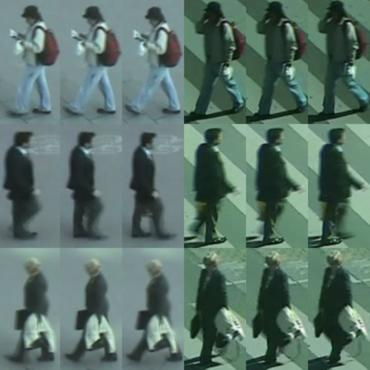
\includegraphics[width=0.4\textwidth]{image/gestion_id}
		\caption{\textbf{Person Re-Identification}}
		\label{gestion_id}
	\end{figure}
	
	
	\section{Propuesta}
	
	El flujo de trabajo que se propone, tiene como fin evaluar y comparar modelos de reidentificación (ReID) en el contexto del análisis deportivo, mediante una secuencia de procesamiento de vídeo que engloba detección, tracking y reidentificación de los jugadores. El flujo de trabajo empieza, por la aplicación de modelos de detección de objetos (bajo YOLOv10 o YOLOX), la obtención de las etiquetas con los modelos de ReID y el algoritmo de asociación GTA-LINK, hasta la obtención de un vídeo con las identidades de los jugadores y un fichero MOT con las trayectorias de los jugadores.
	
	Al extraer esta anotación, tienen que ser los usuarios los que las modifiquen mediante un procedimiento manual, obteniendo un dataset (OIR) para entrenar y evaluar nuevos modelos de ReID en condiciones controladas. La evaluación se efectúa utilizando parámetros estándar como mAP y Rank-k, cuantificando así el rendimiento de los modelos en diferentes escenarios, configuraciones y circunstancias.
	
	\begin{figure}[H]
		\centering
		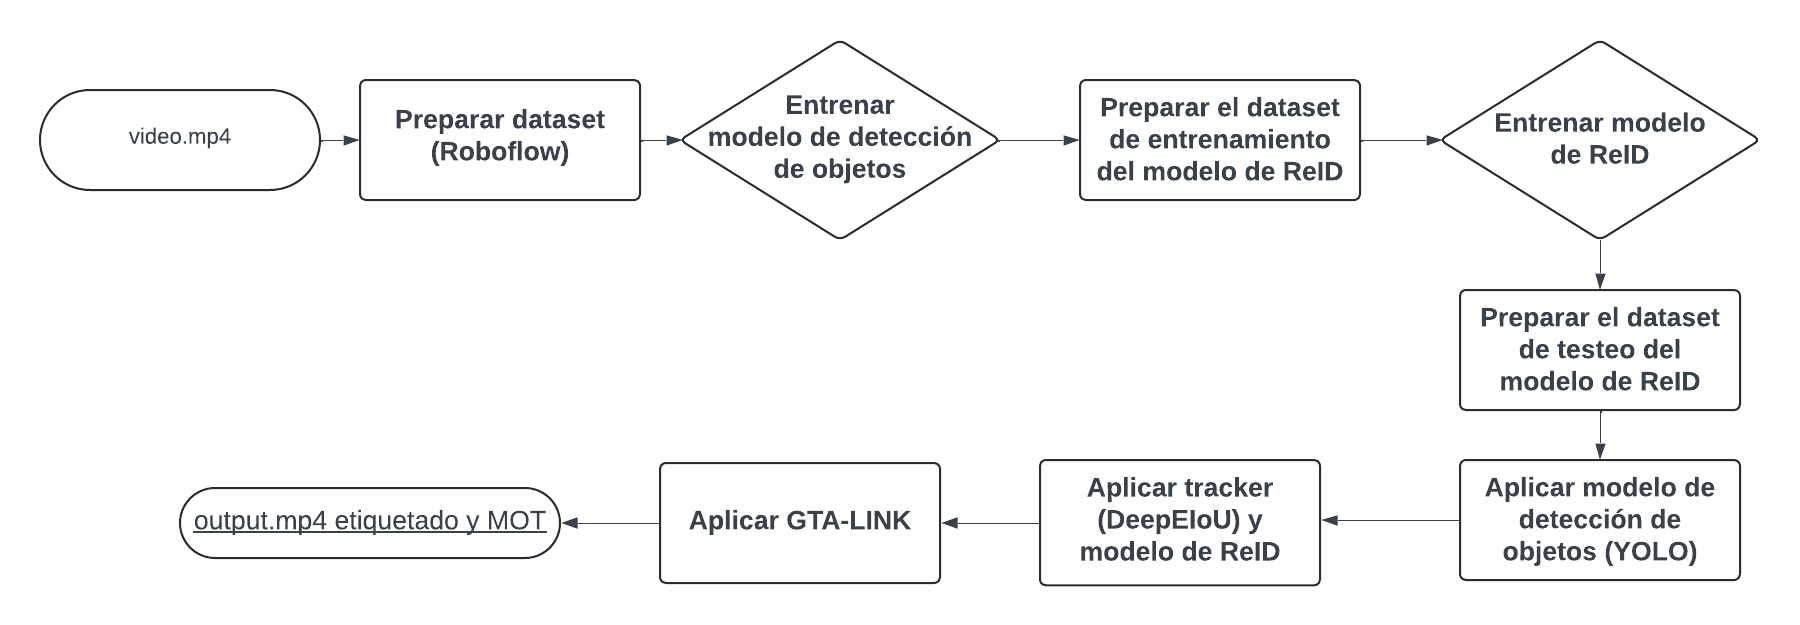
\includegraphics[width=0.8\textwidth]{image/Flowcharts}
		\caption{\textbf{Propuesta}}
		\label{fig:Propuesta}
	\end{figure}
	
	
	\section{Arquitectura general del sistema}
	
	A continuación, se explica paso a paso el flujo completo, desde la entrada de vídeo original hasta la salida final con el vídeo anotado y anotaciones generadas. Cada módulo del sistema se presenta de forma independiente, especificando su función dentro del flujo, la tecnología empleada y los beneficios que aporta al conjunto. \ref{fig:Propuesta}
	
	\subsection{Selección del vídeo de entrada (video.mp4)}
	
	A fin de poder desarrollar y validar el flujo de trabajo que se propone, fue preciso seleccionar un vídeo que contara con las características necesarias para evaluar, de forma conjunta, tanto los modelos para la detección y el seguimiento, como, en particular, aquellos métodos de reidentificación. Para tal fin, optamos por un clip de 52 minutos que extraímos de un partido completo de fútbol amateur de 2 horas de duración.
	
	La elección de este material no fue caprichosa, ya que se procuró explícitamente un segmento que comprendiese muchas entradas y salidas de jugadores en la escena, ya que ese es uno de los aspectos más complicados a los que se enfrentan los sistemas de reidentificación. Los momentos en que se producen las salidas y entradas de jugadores en la escena son especialmente relevantes, en tanto que se requiere que el modelo mantenga la coherencia a la hora de otorgar identidades aun cuando la visibilidad del jugador se interrumpe.
	
	Asimismo, se buscó que las entradas y salidas iban a producirse a profundidades diferentes en el plano de la imagen, o sea, que los jugadores estuvieran a distancias diferentes de la cámara, lo que produciría el efecto de la perspectiva, y que se traduciría en variaciones interesantes en tamaño aparente, resolución, textura visual de los jugadores, para dificultar aún más el trabajo del modelo de ReID. Así, la reidentificación ha de ser capaz de lidiar con discrepancias importantes en la representación visual del mismo individuo en condiciones de entrar o reaparecer.
	
	\subsection{Aplicar modelo de detección de objetos (YOLOX)}
	
	Para aplicar el modelo de detección de objetos YOLOX, se utilizó el código del repositorio \texttt{DeepEIoU}, específicamente el archivo \texttt{demo.py}, junto con una configuración personalizada definida en el archivo \texttt{yolox\_x\_ch\_sportsmot.py}. El objetivo es detectar jugadores en los fotogramas de un vídeo utilizando el modelo YOLOX.
	
	\subsubsection{Configuración del Modelo YOLOX en \texttt{yolox\_x\_ch\_sportsmot.py}}
	
	El archivo \texttt{yolox\_x\_ch\_sportsmot.py} define los parámetros clave del modelo YOLOX, que son cruciales para la detección de objetos en los fotogramas. Los puntos clave de esta configuración son:
	
	\begin{itemize}
		\item \textbf{Número de Clases y Tamaño de Entrada:} El número de clases se establece en 1, ya que solo se está detectando la clase "jugador". El tamaño de la entrada de la imagen se define como (800, 1440), lo que permite trabajar con imágenes de alta resolución.
		\begin{verbatim}
			self.num_classes = 1
			self.input_size = (800, 1440)
			self.test_size = (800, 1440)
		\end{verbatim}
		
		\item \textbf{Parámetros de Evaluación:} Se especifican los umbrales de confianza (\texttt{test\_conf}) y de NMS (\texttt{nmsthre}), que son cruciales para filtrar las detecciones de baja calidad y evitar duplicados en la misma imagen.
		\begin{verbatim}
			self.test_conf = 0.1
			self.nmsthre = 0.7
		\end{verbatim}
		
		\item \textbf{Configuración de Datos y Transformaciones:} Se utiliza la clase \texttt{MOTDataset} para cargar el conjunto de datos de detección de objetos, con las transformaciones definidas en \texttt{TrainTransform} y \texttt{ValTransform} para preprocesar las imágenes de entrada.
		\begin{verbatim}
			dataset = MOTDataset(
			data_dir='/work/hsiangwei/dataset/',
			json_file=self.train_ann,
			name='',
			img_size=self.input_size,
			preproc=TrainTransform(
			rgb_means=(0.485, 0.456, 0.406),
			std=(0.229, 0.224, 0.225),
			max_labels=500,
			),
			)
		\end{verbatim}
	\end{itemize}
	
	\subsubsection{Implementación en \texttt{demo.py}}
	
	El archivo \texttt{demo.py} aplica el modelo YOLOX para realizar la detección de objetos en una secuencia de vídeo. Los aspectos clave de su funcionamiento son:
	
	\begin{itemize}
		\item \textbf{Cargar el Modelo:} El modelo se carga utilizando la configuración definida en el archivo de experimentos, que especifica la arquitectura y los parámetros de entrenamiento. Se utiliza la clase \texttt{Predictor} para gestionar la inferencia.
		\begin{verbatim}
			model = exp.get_model().to(args.device)
			model.eval()
		\end{verbatim}
		
		\item \textbf{Inferencia en Fotogramas de Vídeo:} En cada fotograma del vídeo, se realiza la detección de objetos utilizando el modelo YOLOX. El preprocesamiento de las imágenes se realiza con la función \texttt{preproc}, que ajusta el tamaño de las imágenes y normaliza los valores RGB.
		\begin{verbatim}
			img, ratio = preproc(img, self.test_size, self.rgb_means, self.std)
			img = torch.from_numpy(img).unsqueeze(0).float().to(self.device)
		\end{verbatim}
		
		\item \textbf{Postprocesamiento de Detecciones:} Después de realizar la inferencia, se aplica el postprocesamiento para filtrar las detecciones utilizando los umbrales de confianza y NMS. Esto garantiza que solo se conserven las detecciones más confiables.
		\begin{verbatim}
			outputs = postprocess(
			outputs, self.num_classes, self.confthre, self.nmsthre
			)
		\end{verbatim}
		
		\item \textbf{Visualización de Detecciones:} Finalmente, las detecciones de objetos se visualizan en el fotograma utilizando la función \texttt{plot\_tracking}. Esta función dibuja las cajas delimitadoras alrededor de los jugadores detectados, y puede mostrar el ID del jugador junto con la caja de la detección.
		\begin{verbatim}
			online_im = plot_tracking(
			img_info['raw_img'], online_tlwhs, 
			online_ids, frame_id=frame_id + 1, fps=1. timer.average_time
			)
		\end{verbatim}
	\end{itemize}
	
	
	
	
	\subsection{Aplicar tracker (DeepEIoU) y modelo de reID}
	
	En esta sección, se aplican el tracker Deep-EIoU y el modelo de reidentificación (ReID) para hacer el seguimiento y asociar las detecciones de jugadores a lo largo de los fotogramas de un vídeo.
	
	\subsubsection{Deep-EIoU en \texttt{DeepEIoU.py}}
	
	El archivo \texttt{DeepEIoU.py} contiene la implementación del tracker Deep-EIoU, que utiliza el algoritmo de seguimiento y Kalman filter para asociar las detecciones de objetos a lo largo de los fotogramas. A continuación se describen los puntos clave de su implementación:
	
	\begin{itemize}
		\item \textbf{Clase \texttt{STrack}:}  
		La clase \texttt{STrack} representa un objeto de seguimiento y contiene las características principales, como la predicción de la posición del objeto, la actualización de las características y la gestión de su estado utilizando un filtro de Kalman.
		\vspace{0.5cm}
		\begin{lstlisting}[style=pythonstyle]
			class STrack(BaseTrack):
			shared_kalman = KalmanFilter()
			def __init__(self, tlwh, score, feat=None, feat_history=30):
			...
		\end{lstlisting}
		
		La clase gestiona el estado del objeto (\texttt{tracked}, \texttt{lost}), la actualización de sus características visuales (con el método \texttt{update\_features}) y la predicción de la siguiente posición usando el filtro de Kalman.
		
		\item \textbf{Predicción y Actualización:}  
		La predicción de la siguiente posición de un objeto se realiza usando el filtro de Kalman para predecir su estado y su covarianza. La función \texttt{predict()} actualiza la posición del objeto.
		\vspace{0.5cm}
		\begin{lstlisting}[style=pythonstyle]
			def predict(self):
			self.mean, self.covariance = self.kalman_filter.predict(self.mean, self.covariance)
		\end{lstlisting}
		
		\item \textbf{Activación y Re-activación:}  
		Los objetos se activan al ser detectados por primera vez y se reactivan si han sido perdidos temporalmente. El método \texttt{activate()} inicia un nuevo seguimiento, mientras que \texttt{re\_activate()} se utiliza para volver a activar objetos previamente perdidos.
		\vspace{0.5cm}
		\begin{lstlisting}[style=pythonstyle]
			def activate(self, kalman_filter, frame_id):
			...
			def re_activate(self, new_track, frame_id, new_id=False):
			...
		\end{lstlisting}
		
		\item \textbf{Estado del Objeto:}  
		La propiedad \texttt{tlwh} convierte la posición de los objetos en el formato de caja delimitadora y la propiedad \texttt{xywh} convierte la caja en un formato de coordenadas (centro x, centro y, ancho, altura).
		\vspace{0.5cm}
		\begin{lstlisting}[style=pythonstyle]
			@property
			def tlwh(self):
			...
			@property
			def xywh(self):
			...
		\end{lstlisting}
		
		\item \textbf{Tracker \texttt{Deep\_EIoU}:}  
		El tracker \texttt{Deep\_EIoU} gestiona los objetos detectados y su seguimiento a lo largo de los fotogramas. El método \texttt{update()} actualiza los objetos seguidos, gestiona las asociaciones entre objetos y detecciones, y controla la activación y reactivación de los objetos.
		\vspace{0.5cm}
		\begin{lstlisting}[style=pythonstyle]
			class Deep_EIoU(object):
			def __init__(self, args, frame_rate=30):
			...
			def update(self, output_results, embedding):
			...
		\end{lstlisting}
		\vspace{0.5cm}
		El método \texttt{update()} recibe las detecciones y las características de cada objeto, realiza asociaciones entre los objetos seguidos y las nuevas detecciones, y actualiza el estado de cada objeto.
		
		\item \textbf{Asociación de Detecciones:}  
		La asociación de objetos se realiza utilizando una combinación de la distancia IoU (Intersection over Union) y la distancia en el espacio de características (\texttt{embedding}) de ReID. Los objetos se asocian primero con detecciones de alta puntuación y luego con detecciones de puntuación baja.
		\vspace{0.5cm}
		\begin{lstlisting}[style=pythonstyle]
			ious_dists = matching.eiou_distance(strack_pool, detections, cur_expand_scale)
			matches, u_track, u_detection = matching.linear_assignment(dists, thresh=self.args.match_thresh)
		\end{lstlisting}
		
		\item \textbf{Gestión de la Pérdida de Objetos:}  
		Los objetos perdidos se gestionan mediante el parámetro \texttt{max\_time\_lost}, y se marcan como eliminados si no se han rastreado durante el número máximo de fotogramas permitidos.
		\vspace{0.5cm}
		\begin{lstlisting}[style=pythonstyle]
			for track in self.lost_stracks:
			if self.frame_id - track.end_frame > self.max_time_lost:
			track.mark_removed()
		\end{lstlisting}
	\end{itemize}
	
	\subsubsection{Modelo de Reidentificación (ReID)}
	
	El modelo de ReID se utiliza para asociar objetos detectados en diferentes fotogramas a través de sus características visuales. A continuación, se describe cómo se integran las características de ReID con el tracker Deep-EIoU:
	
	\begin{itemize}
		\item \textbf{Extracción de Características de ReID:}  
		Se extraen características visuales de las detecciones utilizando un extractor de características preentrenado, como el modelo \texttt{osnet\_x1\_0}.
		\vspace{0.5cm}
		\begin{lstlisting}[style=pythonstyle]
			extractor = FeatureExtractor(
			model_name='osnet_x1_0',
			model_path='checkpoints/sports_model.pth.tar-60',
			device='cpu'
			)
		\end{lstlisting}
		\vspace{0.5cm}
		\item \textbf{Asignación de Características a Detecciones:}  
		Las características extraídas se asignan a las detecciones de los jugadores, permitiendo al tracker realizar la reidentificación de los mismos a lo largo de los fotogramas.
		\vspace{0.5cm}
		\begin{lstlisting}[style=pythonstyle]
			cropped_imgs = [frame[max(0,int(y1)):min(height,int(y2)),max(0,int(x1)):min(width,int(x2))] for x1,y1,x2,y2,_,_,_ in det]
			embs = extractor(cropped_imgs)
			embs = embs.cpu().detach().numpy()
		\end{lstlisting}
	\end{itemize}
	
	\subsection{Extraer frames}
	El procedimiento a seguir consiste en la extracción de los fotogramas individuales a partir del vídeo original, para así poder preparar los datos de entrada requeridos por el módulo generate\_tracklets.py del sistema GTA-LINK. Al igual que el resto de módulos, dicho módulo necesita que los frames se encuentren en formato imagen, a partir de los cuales se generarán posteriormente las trayectorias iniciales de los jugadores.
	
	Para conseguirlo se creó el script extract\_frames.py, el cual se dedica a extraer un video (para el caso del presente trabajo, video.mp4 ) y transformarlo en una secuencia ordenada a partir de imágenes numeradas que serán guardado en el folder img1, la cual sigue la especificación de la estructura de carpetas que se sigue en el estándar MOT Challenge necesaria para todos los modelos de detección y seguimiento que se utilizan en el flujo posterior.
	\vspace{0.5cm}
	\begin{lstlisting}[style=pythonstyle]
		import os
		import cv2
		
		def extract_frames(video_path, output_dir):
		"""
		Extrae los frames de un video y los guarda en la estructura MOT Challenge.
		
		Args:
		video_path (str): Ruta al video de entrada (ej: 'video1.mp4').
		output_dir (str): Directorio base de salida (ej: 'frames/').
		"""
		# Crear estructura de directorios (MOT Challenge style)
		seq_name = os.path.splitext(os.path.basename(video_path))[0]  # 'video1' si el input es 'video1.mp4'
		img_dir = os.path.join(output_dir, seq_name, "img1")
		os.makedirs(img_dir, exist_ok=True)
		
		# Abrir video
		cap = cv2.VideoCapture(video_path)
		if not cap.isOpened():
		raise ValueError(f"No se pudo abrir el video: {video_path}")
		
		frame_count = 0
		
		while True:
		ret, frame = cap.read()
		if not ret:
		break
		
		frame_count += 1
		frame_filename = f"{frame_count:06d}.jpg"  # Formato: 000001.jpg, 000002.jpg, ...
		frame_path = os.path.join(img_dir, frame_filename)
		cv2.imwrite(frame_path, frame)
		
		cap.release()
		print(f"{frame_count} frames extraidos y guardados en: {img_dir}")
		
		if __name__ == "__main__":
		import argparse
		parser = argparse.ArgumentParser(description="Extrae frames de un video y los guarda en estructura MOT Challenge.")
		parser.add_argument("--video_path", type=str, required=True, help="Ruta al video de entrada (ej: 'video1.mp4').")
		parser.add_argument("--output_dir", type=str, default="frames", help="Directorio base de salida (ej: 'frames/').")
		args = parser.parse_args()
		
		extract_frames(args.video_path, args.output_dir)
	\end{lstlisting}
	
	\subsection{Aplicar GTA-LINK}
	
	El proceso de seguimiento de objetos en un vídeo puede verse afectado por problemas como cambios de identidad o interrupciones temporales en el seguimiento de jugadores. Para abordar estos desafíos, se aplica el método \textbf{GTA: Global Tracklet Association}. Este enfoque se utiliza para refinar y mejorar la asociación de tracklets generados durante el seguimiento. A través de la aplicación de GTA, es posible corregir problemas como cambios de identidad, fusionar tracklets incorrectos y garantizar una asociación más precisa de los jugadores a lo largo del tiempo.
	
	GTA-LINK permite mejorar el rendimiento del seguimiento de objetos al trabajar sobre los resultados de cualquier modelo de seguimiento, como DeepEIoU. Este proceso de post-procesamiento refina las asociaciones de tracklets mediante dos componentes principales: el \textbf{tracklet splitter} y el \textbf{tracklet connector}. El primero se encarga de dividir tracklets que contienen múltiples identidades utilizando un algoritmo de clustering no supervisado basado en densidad, mientras que el segundo conecta los tracklets correctos mediante el cálculo de distancias promedio entre las características de los tracklets.
	
	La importancia de GTA-LINK radica en su capacidad para corregir y mejorar los resultados de cualquier modelo de seguimiento sin necesidad de modificaciones en el modelo de seguimiento original. En el flujo de trabajo, se emplea este método después de obtener las predicciones iniciales de seguimiento y antes de la reidentificación para garantizar que las asociaciones de tracklets sean lo más precisas posibles.
	
	
	En este apartado del flujo, se utilizan dos scripts principales para generar y refinar los tracklets: \textbf{generate\_tracklets.py} y \textbf{refine\_tracklets.py}. A continuación, se explica cómo funciona cada uno de estos scripts y qué aportan al flujo general de trabajo.
	
	\subsubsection{generate\_tracklets.py}
	
	El script \textbf{generate\_tracklets.py} tiene como objetivo generar tracklets a partir de los resultados de seguimiento y las secuencias originales de fotogramas en formato RGB. Este proceso se realiza de la siguiente manera:
	
	\begin{itemize}
		\item Primero, se carga un extractor de características utilizando el modelo de reidentificación (por ejemplo \texttt{osnet\_x1\_0}). Este modelo es responsable de generar las características que se usarán para asociar las detecciones de los jugadores en cada fotograma.
		\item Se procesan las secuencias de vídeo para obtener las predicciones de seguimiento en cada fotograma. Para cada fotograma, se extraen las características de las detecciones y se actualizan los tracklets existentes.
		\item El script organiza los resultados de las detecciones de cada secuencia en archivos \texttt{.pkl}, que contienen los tracklets de la secuencia, con las características extraídas asociadas a cada uno.
	\end{itemize}
	
	El código esencial del script se muestra a continuación:
	\vspace{0.5cm}
	\begin{lstlisting}[style=pythonstyle]
		def main(model_path, data_path, pred_dir, tracker):
		# Cargar extractor de caracteristicas
		val_transforms = T.Compose([T.Resize([256, 128]), T.ToTensor(), T.Normalize(mean=[0.485, 0.456, 0.406], std=[0.229, 0.224, 0.225])])
		extractor = FeatureExtractor(model_name='osnet_x1_0', model_path=model_path, device=device)
		# Procesar secuencias y generar tracklets
		for s_id, seq in tqdm(enumerate(seqs, 1), total=len(seqs), desc='Processing Seqs'):
		# Iterar sobre los frames y actualizar los tracklets con las detecciones y caracteristicas
		for frame_id in range(1, last_frame+1):
		# Actualizacion de tracklets con las caracteristicas extraidas
		features = extractor(input_batch)
		# Guardar tracklets en archivos .pkl
		with open(track_output_path, 'wb') as f:
		pickle.dump(seq_tracks, f)
	\end{lstlisting}
	
	Este script genera los tracklets a partir de las predicciones del seguimiento, asociando las características extraídas a cada tracklet y guardando los resultados en formato \textbf{pickle}.
	
	\subsubsection{refine\_tracklets.py}
	
	El script \texttt{refine\_tracklets.py} lleva a cabo un tratamiento de los tracklets generados por el sistema de seguimiento que mejora la precisión en la asociación de identidades y corrige los errores más comunes en situaciones difíciles. Este tratamiento es necesario para que puedan ser recuperadas trayectorias coherentes y estables que describan la trayectoria que siguen los jugadores a lo largo del vídeo.
	
	En primer lugar, el componente denominado \textbf{Tracklet Splitter} es el responsable de detectar los tracklets "sucios" o impuros, aquellos tracklets que en alguna de sus detecciones contienen detecciones para distintos jugadores. Utiliza un algoritmo no supervisado de \textit{clustering}, el conocido como DBSCAN (Density-Based Spatial Clustering of Applications with Noise), que agrupa a las detecciones del mismo tracklet en función de la similitud de las características visuales y espaciales de las detecciones. Estas características son entendidas como los \textit{embeddings} extraídos a partir del modelo de reidentificación (los cuales representan la apariencia visual de cada jugador) junto a la información asociada a ellos como pueden ser la posición y tamaño del \textit{bounding box} o el número de frame. En la práctica, al separar estos grupos se evita que un mismo identificador contenga mezclas de jugadores, lo cual garantiza que las trayectorias sean puras y representen únicamente a un jugador.
	
	Una vez realizado el splitting, el Tracklet Connector vuelve a unir aquellos tracklets segregados que se corresponden con la misma persona. La decisión de si dos tracklets deben ser unidos o no se ejerce calculando la distancia de similitud de los embeddings promedios de ambos tracklets, utilizando la distancia de coseno, una métrica que nos permite saber qué tanto se parecen las representaciones de aparición o también como embeddings de las distintas personas. También se tiene en cuenta la distancia temporal y espacial de los tracklets para que la unión de estos objetos sea lógica, o sea se aproximen en el tiempo y el espacio. Esta parte es muy importante, de hecho trata de eliminar la cantidad de cambios de identidad que hemos tenido (ID switches), permitiendo la reconstrucción de trayectorias completas y consistentes para cada jugador a lo largo de toda la secuencia.
	
	Finalmente, una vez conseguido el producto resultante el script obtiene visualizaciones de las distancias entre los tracklets para obtener mapas de calor o heatmaps que enlazan entre sí las distancias entre los tracklets, permitiendo la evaluación visual de la distribución de similitud entre los distintos tracklets y, al mismo tiempo detectar errores en las divisiones o uniones; o a la inversa ajustar parámetros importantes como los umbrales de clustering o fusión.
	
	
	El código esencial de este script es el siguiente:
	\vspace{0.5cm}
	
	\begin{lstlisting}[style=pythonstyle]
		import numpy as np
		import os
		import torch
		import pickle
		
		from collections import defaultdict
		
		import matplotlib.pyplot as plt
		import seaborn as sns
		
		from loguru import logger
		from tqdm import tqdm
		
		from sklearn.cluster import DBSCAN
		from sklearn.preprocessing import StandardScaler
		from scipy.spatial.distance import cdist
		
		from Tracklet import Tracklet
		
		import argparse
		
		def find_consecutive_segments(track_times):
		"""
		Identifies and returns the start and end indices of consecutive segments in a list of times.
		
		Args:
		track_times (list): A list of frame times (integers) representing when a tracklet was detected.
		
		Returns:
		list of tuples: Each tuple contains two integers (start_index, end_index) representing the start and end of a consecutive segment.
		"""
		segments = []
		start_index = 0
		end_index = 0
		for i in range(1, len(track_times)):
		if track_times[i] == track_times[end_index] + 1:
		end_index = i
		else:
		segments.append((start_index, end_index))
		start_index = i
		end_index = i
		segments.append((start_index, end_index))
		return segments
		
		def query_subtracks(seg1, seg2, track1, track2):
		"""
		Processes and pairs up segments from two different tracks to form valid subtracks based on their temporal alignment.
		
		Args:
		seg1 (list of tuples): List of segments from the first track where each segment is a tuple of start and end indices.
		seg2 (list of tuples): List of segments from the second track similar to seg1.
		track1 (Tracklet): First track object containing times and bounding boxes.
		track2 (Tracklet): Second track object similar to track1.
		
		Returns:
		list: Returns a list of subtracks which are either segments of track1 or track2 sorted by time.
		"""
		subtracks = []  # List to store valid subtracks
		while seg1 and seg2:  # Continue until seg1 or seg1 is empty
		s1_start, s1_end = seg1[0]  # Get the start and end indices of the first segment in seg1
		s2_start, s2_end = seg2[0]  # Get the start and end indices of the first segment in seg2
		'''Optionally eliminate false positive subtracks
		if (s1_end - s1_start + 1) < 30:
		seg1.pop(0)  # Remove the first element from seg1
		continue
		if (s2_end - s2_start + 1) < 30:
		seg2.pop(0)  # Remove the first element from seg2
		continue
		'''
		
		subtrack_1 = track1.extract(s1_start, s1_end)
		subtrack_2 = track2.extract(s2_start, s2_end)
		
		s1_startFrame = track1.times[s1_start]  # Get the starting frame of subtrack 1
		s2_startFrame = track2.times[s2_start]  # Get the starting frame of subtrack 2
		
		# print("track 1 and 2 start frame:", s1_startFrame, s2_startFrame)
		# print("track 1 and 2 end frame:", track1.times[s1_end], track2.times[s2_end])
		
		if s1_startFrame < s2_startFrame:  # Compare the starting frames of the two subtracks
		assert track1.times[s1_end] <= s2_startFrame
		subtracks.append(subtrack_1)
		subtracks.append(subtrack_2)
		else:
		assert s1_startFrame >= track2.times[s2_end]
		subtracks.append(subtrack_2)
		subtracks.append(subtrack_1)
		seg1.pop(0)
		seg2.pop(0)
		
		seg_remain = seg1 if seg1 else seg2
		track_remain = track1 if seg1 else track2
		while seg_remain:
		s_start, s_end = seg_remain[0]
		if(s_end - s_start) < 30:
		seg_remain.pop(0)
		continue
		subtracks.append(track_remain.extract(s_start, s_end))
		seg_remain.pop(0)
		
		return subtracks  # Return the list of valid subtracks sorted ascending temporally
		
		def get_subtrack(track, s_start, s_end):
		"""
		Extracts a subtrack from a given track.
		
		Args:
		track (STrack): The original track object from which the subtrack is to be extracted.
		s_start (int): The starting index of the subtrack.
		s_end (int): The ending index of the subtrack.
		
		Returns:
		STrack: A subtrack object extracted from the original track object, containing the specified time intervals
		and bounding boxes. The parent track ID is also assigned to the subtrack.
		"""
		subtrack = Tracklet()
		subtrack.times = track.times[s_start : s_end + 1]
		subtrack.bboxes = track.bboxes[s_start : s_end + 1]
		subtrack.parent_id = track.track_id
		
		return subtrack
		
		def get_spatial_constraints(tid2track, factor):
		"""
		Calculates and returns the maximal spatial constraints for bounding boxes across all tracks.
		
		Args:
		tid2track (dict): Dictionary mapping track IDs to their respective track objects.
		factor (float): Factor by which to scale the calculated x and y ranges.
		
		Returns:
		tuple: Maximal x and y range scaled by the given factor.
		"""
		
		min_x = float('inf')
		max_x = -float('inf')
		min_y = float('inf')
		max_y = -float('inf')
		
		for track in tid2track.values():
		for bbox in track.bboxes:
		assert len(bbox) == 4
		x, y, w, h = bbox[0:4]  # x, y is coordinate of top-left point of bounding box
		x += w / 2  # get center point
		y += h / 2  # get center point
		min_x = min(min_x, x)
		max_x = max(max_x, x)
		min_y = min(min_y, y)
		max_y = max(max_y, y)
		
		x_range = abs(max_x - min_x) * factor
		y_range = abs(max_y - min_y) * factor
		
		return x_range, y_range
		
		def display_Dist(Dist, seq_name=None, isMerged=False, isSplit=False):
		"""
		Displays a heatmap for the distances between tracklets for one or more sequences.
		
		Args:
		seq2Dist (dict): A dictionary mapping sequence names to their corresponding distance matrices.
		seq_name (str, optional): Specific sequence name to display the heatmap for. If None, displays for all sequences.
		isMerged (bool): Flag indicating whether the distances are post-merge.
		isSplit (bool): Flag indicating whether the distances are post-split.
		"""
		split_info = " After Split" if isSplit else " Before Split"
		merge_info = " After Merge" if isMerged else " Before Merge"
		info = split_info + merge_info
		
		plt.figure(figsize=(10, 8))  # Optional: adjust the size of the heatmap
		
		# Plot the heatmap
		sns.heatmap(Dist, cmap='Blues')
		
		plt.title(f"{seq_name}{info}")
		plt.show()
		
		def get_distance_matrix(tid2track):
		"""
		Constructs and returns a distance matrix between all tracklets based on overlapping times and feature similarities.
		
		Args:
		tid2track (dict): Dictionary mapping track IDs to their respective track objects.
		
		Returns:
		ndarray: A square matrix where each element (i, j) represents the calculated distance between track i and track j.
		"""
		# print("number of tracks:", len(tid2track))
		Dist = np.zeros((len(tid2track), len(tid2track)))
		
		for i, (track1_id, track1) in enumerate(tid2track.items()):
		assert len(track1.times) == len(track1.bboxes)
		for j, (track2_id, track2) in enumerate(tid2track.items()):
		if j < i:
		Dist[i][j] = Dist[j][i]
		else:
		Dist[i][j] = get_distance(track1_id, track2_id, track1, track2)
		return Dist
		
		def get_distance(track1_id, track2_id, track1, track2):
		"""
		Calculates the cosine distance between two tracks using PyTorch for efficient computation.
		
		Args:
		track1_id (int): ID of the first track.
		track2_id (int): ID of the second track.
		track1 (Tracklet): First track object.
		track2 (Tracklet): Second track object.
		
		Returns:
		float: Cosine distance between the two tracks.
		"""
		assert track1_id == track1.track_id and track2_id == track2.track_id   # debug line
		doesOverlap = False
		if (track1_id != track2_id):
		doesOverlap = set(track1.times) & set(track2.times)
		if doesOverlap:
		return 1                # make the cosine distance between two tracks maximum, max = 1
		else:
		# calculate cosine distance between two tracks based on features
		device = torch.device("cuda" if torch.cuda.is_available() else "cpu")
		track1_features_tensor = torch.tensor(np.stack(track1.features), dtype=torch.float32).to(device)
		track2_features_tensor = torch.tensor(np.stack(track2.features), dtype=torch.float32).to(device)
		count1 = len(track1_features_tensor)
		count2 = len(track2_features_tensor)
		
		cos_sim_Numerator = torch.matmul(track1_features_tensor, track2_features_tensor.T)
		track1_features_dist = torch.norm(track1_features_tensor, p=2, dim=1, keepdim=True)
		track2_features_dist = torch.norm(track2_features_tensor, p=2, dim=1, keepdim=True)
		cos_sim_Denominator = torch.matmul(track1_features_dist, track2_features_dist.T)
		cos_Dist = 1 - cos_sim_Numerator / cos_sim_Denominator
		
		total_cos_Dist = cos_Dist.sum()
		result = total_cos_Dist / (count1 * count2)
		return result
		
		def check_spatial_constraints(trk_1, trk_2, max_x_range, max_y_range):
		"""
		Checks if two tracklets meet spatial constraints for potential merging.
		
		Args:
		trk_1 (Tracklet): The first tracklet object containing times and bounding boxes.
		trk_2 (Tracklet): The second tracklet object containing times and bounding boxes, to be evaluated
		against trk_1 for merging possibility.
		max_x_range (float): The maximum allowed distance in the x-coordinate between the end of trk_1 and
		the start of trk_2 for them to be considered for merging.
		max_y_range (float): The maximum allowed distance in the y-coordinate under the same conditions as
		the x-coordinate.
		
		Returns:
		bool: True if the spatial constraints are met (the tracklets are close enough to consider merging),
		False otherwise.
		"""
		inSpatialRange = True
		seg_1 = find_consecutive_segments(trk_1.times)
		seg_2 = find_consecutive_segments(trk_2.times)
		'''Debug
		assert((len(seg_1) + len(seg_2)) > 1)         # debug line, delete later
		print(seg_1)                                  # debug line, delete later
		print(seg_2)                                  # debug line, delete later
		'''
		
		subtracks = query_subtracks(seg_1, seg_2, trk_1, trk_2)
		# assert(len(subtracks) > 1)                    # debug line, delete later
		subtrack_1st = subtracks.pop(0)
		# print("Entering while loop")
		while subtracks:
		# print("Subtracks remaining: ", len(subtracks))
		subtrack_2nd = subtracks.pop(0)
		if subtrack_1st.parent_id == subtrack_2nd.parent_id:
		subtrack_1st = subtrack_2nd
		continue
		x_1, y_1, w_1, h_1 = subtrack_1st.bboxes[-1][0 : 4]
		x_2, y_2, w_2, h_2 = subtrack_2nd.bboxes[0][0 : 4]
		x_1 += w_1 / 2
		y_1 += h_1 / 2
		x_2 += w_2 / 2
		y_2 += h_2 / 2
		dx = abs(x_1 - x_2)
		dy = abs(y_1 - y_2)
		
		# check the distance between exit location of track_1 and enter location of track_2
		if dx > max_x_range or dy > max_y_range:
		inSpatialRange = False
		# print(f"dx={dx}, dy={dy} out of range max_x_range = {max_x_range}, max_y_range  = {max_y_range}")    # debug line, delete later
		break
		else:
		subtrack_1st = subtrack_2nd
		# print("Exit while loop")
		return inSpatialRange
		
		def merge_tracklets(tracklets, seq2Dist, Dist, seq_name=None, max_x_range=None, max_y_range=None, merge_dist_thres=None):
		seq2Dist[seq_name] = Dist                               # save all seqs distance matrix, debug line, delete later
		# displayDist(seq2Dist, seq_name, isMerged=False, isSplit=True)         # used to display Dist, debug line, delete later=
		
		idx2tid = {idx: tid for idx, tid in enumerate(tracklets.keys())}
		
		# Hierarchical Clustering
		# While there are still values (exclude diagonal) in distance matrix lower than merging distance threshold
		#   Step 1: find minimal distance for tracklet pair
		#   Step 2: merge tracklet pair
		#   Step 3: update distance matrix
		diagonal_mask = np.eye(Dist.shape[0], dtype=bool)
		non_diagonal_mask = ~diagonal_mask
		# print("Enter merge while loop")
		while (np.any(Dist[non_diagonal_mask] < merge_dist_thres)):
		# print(np.sum(np.any(Dist[non_diagonal_mask] < merge_dist_thres)))
		# Get the indices of the minimum value considering the mask
		min_index = np.argmin(Dist[non_diagonal_mask])
		min_value = np.min(Dist[non_diagonal_mask])
		# Translate this index to the original array's indices
		masked_indices = np.where(non_diagonal_mask)
		track1_idx, track2_idx = masked_indices[0][min_index], masked_indices[1][min_index]
		# print("Tracks idx to merge:", track1_idx, track2_idx)
		# print(f"Minimum value in masked Dist: {min_value}")
		# print(f"Corresponding value in Dist using recalculated indices: {Dist[track1_idx, track2_idx]}")
		
		assert min_value == Dist[track1_idx, track2_idx] == Dist[track2_idx, track1_idx], "Values should match!"
		
		track1 = tracklets[idx2tid[track1_idx]]
		track2 = tracklets[idx2tid[track2_idx]]
		
		inSpatialRange = check_spatial_constraints(track1, track2, max_x_range, max_y_range)
		# print("In spatial range:", inSpatialRange)
		if inSpatialRange:
		track1.features += track2.features      # Note: currently we merge track 2 to track 1 without creating a new track
		track1.times += track2.times
		track1.bboxes += track2.bboxes
		
		# update tracklets dictionary
		tracklets[idx2tid[track1_idx]] = track1
		tracklets.pop(idx2tid[track2_idx])
		
		# Remove the merged tracklet (track2) from the distance matrix
		Dist = np.delete(Dist, track2_idx, axis=0)  # Remove row for track2
		Dist = np.delete(Dist, track2_idx, axis=1)  # Remove column for track2
		# update idx2tid
		idx2tid = {idx: tid for idx, tid in enumerate(tracklets.keys())}
		
		# Update distance matrix only for the merged tracklet's row and column
		for idx in range(Dist.shape[0]):
		Dist[track1_idx, idx] = get_distance(idx2tid[track1_idx], idx2tid[idx], tracklets[idx2tid[track1_idx]], tracklets[idx2tid[idx]])
		Dist[idx, track1_idx] = Dist[track1_idx, idx]  # Ensure symmetry
		
		seq2Dist[seq_name] = Dist                   # used to display Dist
		
		# update mask
		diagonal_mask = np.eye(Dist.shape[0], dtype=bool)
		non_diagonal_mask = ~diagonal_mask
		else:
		# change distance between track pair to threshold
		Dist[track1_idx, track2_idx], Dist[track2_idx, track1_idx] = merge_dist_thres, merge_dist_thres
		# print("Finish merge while loop")
		return tracklets
		
		def detect_id_switch(embs, eps=None, min_samples=None, max_clusters=None):
		"""
		Detects identity switches within a tracklet using clustering.
		
		Args:
		embs (list of numpy arrays): A list where each element is a numpy array representing an embedding.
		Each embedding has the same dimensionality.
		eps (float): The maximum distance between two samples for one to be considered as in the neighborhood of the other.
		min_samples (int): The number of samples in a neighborhood for a point to be considered as a core point.
		
		Returns:
		bool: True if an identity switch is detected, otherwise False.
		"""
		if len(embs) > 15000:
		embs = embs[1::2]
		
		embs = np.stack(embs)
		
		# Standardize the embeddings
		scaler = StandardScaler()
		embs_scaled = scaler.fit_transform(embs)
		
		# Apply DBSCAN clustering
		db = DBSCAN(eps=eps, min_samples=min_samples, metric='cosine').fit(embs_scaled)
		labels = db.labels_
		
		# Count the number of clusters (excluding noise)
		unique_labels = np.unique(labels)
		unique_labels = unique_labels[unique_labels != -1]
		
		if -1 in labels and len(unique_labels) > 1:
		# Find the cluster centers
		cluster_centers = np.array([embs_scaled[labels == label].mean(axis=0) for label in unique_labels])
		
		# Assign noise points to the nearest cluster
		noise_indices = np.where(labels == -1)[0]
		for idx in noise_indices:
		distances = cdist([embs_scaled[idx]], cluster_centers, metric='cosine')
		nearest_cluster = np.argmin(distances)
		labels[idx] = list(unique_labels)[nearest_cluster]
		
		n_clusters = len(unique_labels)
		
		if max_clusters and n_clusters > max_clusters:
		# Merge clusters to ensure the number of clusters does not exceed max_clusters
		while n_clusters > max_clusters:
		cluster_centers = np.array([embs_scaled[labels == label].mean(axis=0) for label in unique_labels])
		distance_matrix = cdist(cluster_centers, cluster_centers, metric='cosine')
		np.fill_diagonal(distance_matrix, np.inf)  # Ignore self-distances
		
		# Find the closest pair of clusters
		min_dist_idx = np.unravel_index(np.argmin(distance_matrix), distance_matrix.shape)
		cluster_to_merge_1, cluster_to_merge_2 = unique_labels[min_dist_idx[0]], unique_labels[min_dist_idx[1]]
		
		# Merge the clusters
		labels[labels == cluster_to_merge_2] = cluster_to_merge_1
		unique_labels = np.unique(labels)
		unique_labels = unique_labels[unique_labels != -1]
		n_clusters = len(unique_labels)
		
		return n_clusters > 1, labels
		
		def split_tracklets(tmp_trklets, eps=None, max_k=None, min_samples=None, len_thres=None):
		"""
		Splits each tracklet into multiple tracklets based on an internal distance threshold.
		
		Args:
		tmp_trklets (dict): Dictionary of tracklets to be processed.
		eps (float): The maximum distance between two samples for one to be considered as in the neighborhood of the other.
		min_samples (int): The number of samples in a neighborhood for a point to be considered as a core point.
		len_thres (int): Length threshold to filter out short tracklets.
		max_k (int): Maximum number of clusters to consider.
		
		Returns:
		dict: New dictionary of tracklets after splitting.
		"""
		new_id = max(tmp_trklets.keys()) + 1
		tracklets = defaultdict()
		# Splitting algorithm to process every tracklet in a sequence
		for tid in tqdm(sorted(list(tmp_trklets.keys())), total=len(tmp_trklets), desc="Splitting tracklets"):
		# print("Track ID:\n", tid)               # debug line, delete later
		trklet = tmp_trklets[tid]
		if len(trklet.times) < len_thres:  # NOTE: Set tracklet length threshold to filter out short ones
		tracklets[tid] = trklet
		else:
		embs = np.stack(trklet.features)
		frames = np.array(trklet.times)
		bboxes = np.stack(trklet.bboxes)
		scores = np.array(trklet.scores)
		# Perform DBSCAN clustering
		id_switch_detected, clusters = detect_id_switch(embs, eps=eps, min_samples=min_samples, max_clusters=max_k)
		if not id_switch_detected:
		tracklets[tid] = trklet
		else:
		unique_labels = set(clusters)
		
		for label in unique_labels:
		if label == -1:
		continue  # Skip noise points
		tmp_embs = embs[clusters == label]
		tmp_frames = frames[clusters == label]
		tmp_bboxes = bboxes[clusters == label]
		tmp_scores = scores[clusters == label]
		assert new_id not in tmp_trklets
		
		tracklets[new_id] = Tracklet(new_id, tmp_frames.tolist(), tmp_scores.tolist(), tmp_bboxes.tolist(), feats=tmp_embs.tolist())
		new_id += 1
		
		assert len(tracklets) >= len(tmp_trklets)
		return tracklets
		
		
		def save_results(sct_output_path, tracklets):
		"""
		Saves the final tracklet results into a specified path.
		
		Args:
		sct_output_path (str): Path where the results will be saved.
		tracklets (dict): Dictionary of tracklets containing their final states.
		
		"""
		results = []
		
		for i, tid in enumerate(sorted(tracklets.keys())): # add each track to results
		track = tracklets[tid]
		tid = i + 1
		for instance_idx, frame_id in enumerate(track.times):
		bbox = track.bboxes[instance_idx]
		
		results.append(
		[frame_id, tid, bbox[0], bbox[1], bbox[2], bbox[3], 1, -1, -1, -1]
		)
		results = sorted(results, key=lambda x: x[0])
		txt_results = []
		for line in results:
		txt_results.append(
		f"{line[0]},{line[1]},{line[2]:.2f},{line[3]:.2f},{line[4]:.2f},{line[5]:.2f},{line[6]},{line[7]},{line[8]},{line[9]}\n"
		)
		
		# NOTE: uncomment to save results
		with open(sct_output_path, 'w') as f:
		f.writelines(txt_results)
		logger.info(f"save SCT results to {sct_output_path}")
		
		def parse_args():
		parser = argparse.ArgumentParser(description="Global tracklet association with splitting and connecting.")
		parser.add_argument('--dataset',
		type=str,
		required=True,
		help='Dataset name (e.g., SportsMOT, SoccerNet).')
		
		parser.add_argument('--tracker',
		type=str,
		required=True,
		help='Tracker name.')
		
		parser.add_argument('--track_src',
		type=str,
		default=r"C:\Users\Ciel Sun\OneDrive - UW\EE 599\SoccerNet\SORT_results\SORT_Tracklets_test",
		required=True,
		help='Source directory of tracklet pkl files.'
		)
		
		parser.add_argument('--use_split',
		action='store_true',
		help='If using split component.')
		
		parser.add_argument('--min_len',
		type=int,
		default=100,
		help='Minimum length for a tracklet required for splitting.')
		
		parser.add_argument('--eps',
		type=float,
		default=0.7,
		help='For DBSCAN clustering, the maximum distance between two samples for one to be considered as in the neighborhood of the other.')
		
		parser.add_argument('--min_samples',
		type=int,
		default=10,
		help='The number of samples (or total weight) in a neighborhood for a point to be considered as a core point.')
		
		parser.add_argument('--max_k',
		type=int,
		default=3,
		help='Maximum number of clusters/subtracklets to be output by splitting component.')
		
		parser.add_argument('--use_connect',
		action='store_true',
		help='If using connecting component.')
		
		parser.add_argument('--spatial_factor',
		type=float,
		default=1,
		help='Factor to adjust spatial distances.')
		
		parser.add_argument('--merge_dist_thres',
		type=float,
		default=0.4,
		help='Minimum cosine distance between two tracklets for merging.')
		return parser.parse_args()
		
		def main():
		args = parse_args()
		# Determine the process based on the flags
		if args.use_split and args.use_connect:
		process = "Split+Connect"
		elif args.use_split:
		process = "Split"
		elif args.use_connect:
		process = "Connect"
		else:
		raise ValueError("Both use_split and use_connect are false, must at least use connect.")
		
		seq_tracks_dir = args.track_src
		data_path = os.path.dirname(seq_tracks_dir)
		seqs_tracks = os.listdir(seq_tracks_dir)
		
		tracker = args.tracker
		dataset = args.dataset
		
		seqs_tracks.sort()
		seq2Dist = dict()
		
		process_limit = 10000                          # debug line, delete later
		for seq_idx, seq in enumerate(seqs_tracks):
		if seq_idx >= process_limit:            # debug line, delete later
		break                               # debug line, delete later
		
		seq_name = seq.split('.')[0]
		logger.info(f"Processing seq {seq_idx+1} / {len(seqs_tracks)}")
		with open(os.path.join(seq_tracks_dir, seq), 'rb') as pkl_f:
		tmp_trklets = pickle.load(pkl_f)     # dict(key:track id, value:tracklet)
		
		max_x_range, max_y_range = get_spatial_constraints(tmp_trklets, args.spatial_factor)
		
		# Dist = get_distance_matrix(tmp_trklets)
		# seq2Dist[seq_name] = Dist                                              # save all seqs distance matrix, debug line, delete later
		# display_Dist(Dist, seq_name, isMerged=False, isSplit=False)         # used to display Dist, debug line, delete later
		
		if args.use_split:
		print(f"----------------Number of tracklets before splitting: {len(tmp_trklets)}----------------")
		splitTracklets = split_tracklets(tmp_trklets, eps=args.eps, max_k=args.max_k, min_samples=args.min_samples, len_thres=args.min_len)
		else:
		splitTracklets = tmp_trklets
		
		Dist = get_distance_matrix(splitTracklets)
		# display_Dist(Dist, seq_name, isMerged=False, isSplit=True)
		print(f"----------------Number of tracklets before merging: {len(splitTracklets)}----------------")
		
		mergedTracklets = merge_tracklets(splitTracklets, seq2Dist, Dist, seq_name=seq_name, max_x_range=max_x_range, max_y_range=max_y_range, merge_dist_thres=args.merge_dist_thres)
		# Dist = get_distance_matrix(mergedTracklets)
		# display_Dist(Dist, seq_name, isMerged=True, isSplit=True)
		print(f"----------------Number of tracklets after merging: {len(mergedTracklets)}----------------")
		
		sct_name = f'{tracker}_{dataset}_{process}_eps{args.eps}_minSamples{args.min_samples}_K{args.max_k}_mergeDist{args.merge_dist_thres}_spatial{args.spatial_factor}'
		os.makedirs(os.path.join(data_path, sct_name), exist_ok=True)
		new_sct_output_path = os.path.join(data_path, sct_name, '{}.txt'.format(seq_name))
		save_results(new_sct_output_path, mergedTracklets)
		
		if __name__ == "__main__":
		main()
		
	\end{lstlisting}
	
	Este script se encarga de mejorar los tracklets mediante la fusión y la división de tracklets en función de sus características y la similitud espacial. Esto mejora la precisión del seguimiento de jugadores en el vídeo.
	
	\subsection{Generar el output.mp4 y MOT}
	
	Una vez que se hace el procedimiento correspondiente tanto a la etapa de seguimiento como a la de refinamiento por medio de GTA-LINK —archivo refine\_tracklets.py— se genera un archivo MOT en un formato de texto plano (.txt) con el resultado final que contiene por fotograma las trayectorias finales de los jugadores y también las IDs asignadas. El fichero resultante es sencillamente un archivo de texto plano que no arroja una representación visual del resultado deseado.
	
	Para remediar esta limitación se utilizó el script visualize2.py cuya finalidad es conseguir la visualización de resultado tanto para poder validar el resultado visualmente como para obtener el resultado para su visualización. Este script puede leer como entrada el fichero MOT producido por medio de GTA-LINK y la carpeta img1 donde se encuentren guardados los fotogramas originales y produce un nuevo conjunto de imágenes donde se generan las cajas con las IDs de cada jugador. De forma que se obtiene una nueva secuencia de imágenes con los contornos del resultado final.
	
	Durante este proceso, la ID es rendida con un color aleatorio pero constante para poder seguir el jugador indicando el recorrido durante la reproducción del video. Para cada uno de los fotogramas de vídeo se generan las cajas y textos y se guardan con las imágenes en un directorio definido por el usuario. Llevando a completar así una representación completamente visualizada con la información que existe en el fichero MOT.
	
	Visualize2.py:
	\vspace{0.5cm}
	\begin{lstlisting}[style=pythonstyle]
		import os
		import cv2
		import random
		from tqdm import tqdm
		
		# Configuracion de rutas
		
		tracklet_file = r"C:\Users\jismbs\Documents\gta-link\DeepEIoU_SoccerNet_Split+Connect_eps0.8_minSamples10_K4_mergeDist0.7_spatial1.0\video2_mydata.txt"
		image_folder = r"C:\Users\jismbs\Documents\gta-link\frames_trackerVideo2DeepEIoU_osnet_ImageNet_Soccernet\video2\img1"
		output_folder = r"C:\Users\jismbs\Documents\gta-link\osnetMyData+gta_link"
		
		
		os.makedirs(output_folder, exist_ok=True)
		
		# 1. Cargar tracklets (convertir valores decimales a enteros)
		print("Cargando datos de tracklets...")
		detections = {}
		colors = {}
		
		with open(tracklet_file, 'r') as f:
		for line in f:
		parts = line.strip().split(',')
		try:
		# Convertir a float primero y luego a int para manejar valores como "1.0"
		frame_id = int(float(parts[0]))
		track_id = int(float(parts[1]))
		x, y, w, h = map(float, parts[2:6])
		
		if track_id not in colors:
		colors[track_id] = (
		random.randint(50, 200),
		random.randint(50, 200),
		random.randint(50, 200)
		)
		
		if frame_id not in detections:
		detections[frame_id] = []
		detections[frame_id].append((track_id, int(x), int(y), int(w), int(h)))
		except (ValueError, IndexError) as e:
		print(f"Advertencia: Error al procesar linea - {line.strip()}. Error: {e}")
		continue
		
		# 2. Procesar frames
		print("\nGenerando visualizaciones...")
		for frame_id in tqdm(sorted(detections.keys()), desc="Procesando frames"):
		img_path = os.path.join(image_folder, f"{frame_id:06d}.jpg")
		if not os.path.exists(img_path):
		continue
		
		img = cv2.imread(img_path)
		
		for track_id, x, y, w, h in detections[frame_id]:
		color = colors[track_id]
		
		# Bounding box
		cv2.rectangle(img, (x, y), (x + w, y + h), color, 2)
		
		# Etiqueta con ID
		label = f"ID:{track_id}"
		(text_width, text_height), _ = cv2.getTextSize(label, cv2.FONT_HERSHEY_SIMPLEX, 0.6, 1)
		cv2.rectangle(img, (x, y - text_height - 10), (x + text_width, y), color, -1)
		cv2.putText(img, label, (x, y - 5), cv2.FONT_HERSHEY_SIMPLEX, 0.6, (255,255,255), 1)
		
		cv2.imwrite(os.path.join(output_folder, f"{frame_id:06d}.jpg"), img)
		
		print(f"\nVisualizacion completada. Resultados en:\n{output_folder}")
	\end{lstlisting}
	\vspace{0.5cm}
	Por último, a partir de las imágenes anotadas que ya aparecen generadas con visualize2.py se recurrió al script videomakerByFrame.py para hacer la reconstrucción del archivo final en formato de video. Este script va recuperando las imágenes ordenadas e irlas concatenando a un determinado frame rate constante de 30 FPS y el resultado es un archivo output.mp4que representa el resultado del seguimiento y reidentificación desde una perspectiva visual e interpretable.
	
	videomakerByFrame.py:
	\vspace{0.5cm}
	\begin{lstlisting}[style=pythonstyle]
		import cv2
		import os
		from tqdm import tqdm  # Importar tqdm para la barra de progreso
		
		# Ruta a la carpeta con las imagenes procesadas
		img_folder = r"C:\Users\jismbs\Documents\path\to\SoccerNet\tracking\test\tracked_output"
		
		# Ruta de salida para el video
		output_video = os.path.join(img_folder, "output_video.mp4")
		
		# Obtener la lista de imagenes ordenadas (recorriendo subcarpetas)
		images = []
		for root, dirs, files in os.walk(img_folder):
		for file in files:
		if file.endswith(".jpg"):
		images.append(os.path.join(root, file))
		
		# Verificar si se encontraron imagenes
		if not images:
		print("No se encontraron imagenes en la carpeta.")
		exit()
		
		# Ordenar las imagenes por nombre para asegurar el orden correcto
		images = sorted(images)
		
		# Leer la primera imagen para obtener las dimensiones
		first_image = cv2.imread(images[0])
		height, width, _ = first_image.shape
		
		# Configurar el video (30 FPS)
		fourcc = cv2.VideoWriter_fourcc(*'mp4v')  # Codec para MP4
		video = cv2.VideoWriter(output_video, fourcc, 30, (width, height))
		
		# Usar tqdm para mostrar la barra de carga mientras agregamos las imagenes al video
		for img_path in tqdm(images, desc="Creando video", ncols=100):
		frame = cv2.imread(img_path)
		video.write(frame)
		
		# Liberar el video
		video.release()
		print(f"Video guardado en: {output_video}")
	\end{lstlisting}
	\vspace{0.5cm}
	
	\subsection{Correción de las anotaciones de output.mp4 (MOT)}
	
	El manejo de errores relacionados con la asignación incorrecta de IDs es un paso crucial en el proceso de reidentificación (ReID). Para resolver este problema, se utilizó un enfoque interactivo en el que se corrigen manualmente los errores de asignación de IDs en las anotaciones generadas por el modelo de ReID previamente entrenado con el dataset de SportMOT, que contiene imágenes de fútbol profesional.
	
	\subsubsection{annotate\_review.py}
	
	En primer lugar, las anotaciones de un partido de fútbol amateur fueron generadas utilizando el modelo de ReID entrenado con el dataset de SportMOT. Posteriormente, estas anotaciones fueron procesadas para corregir posibles errores de asignación de IDs. El código utilizado para este proceso interactivo es  y es el siguiente:
	
	\begin{verbatim}
		import os
		import cv2
		import argparse
		import tkinter as tk
		from tkinter import simpledialog
		from collections import Counter
		
		# Interactive MOT correction with flexible ID modification and distinct duplicate coloring
		
		def parse_mot_file(mot_path):
		entries = []
		with open(mot_path, 'r') as f:
		for line in f:
		if not line.strip(): continue
		parts = line.strip().split(',')
		entries.append({
			'frame': int(float(parts[0])), 
			'id': int(float(parts[1])), 
			'bbox': tuple(map(float, parts[2:6])),
			'raw': line.strip()
		})
		return entries
		
		
		def draw_annotations(img, detections, global_highlight=None, raw_color_map=None):
		out = img.copy()
		global_h = set(global_highlight or [])
		for det in detections:
		x, y, w, h = map(int, det['bbox'])
		tid = det['id']
		raw = det['raw']
		if raw_color_map and raw in raw_color_map:
		color = raw_color_map[raw]
		elif tid in global_h:
		color = (0, 0, 255)
		else:
		color = (0, 255, 0)
		cv2.rectangle(out, (x, y), (x + w, y + h), color, 2)
		cv2.putText(out, str(tid), (x, y - 5), cv2.FONT_HERSHEY_SIMPLEX, 0.5, color, 2)
		return out
	\end{verbatim}
	
	Este código permite corregir las asignaciones incorrectas de IDs mediante una interfaz gráfica que permite al usuario modificar o eliminar detecciones, asignar nuevos IDs a instancias específicas, y aprobar o eliminar duplicados.
	
	\textbf{Interacción del usuario:} La interacción con el programa es completamente visual e intuitiva. Al ejecutar el código, el usuario puede visualizar las detecciones en cada fotograma del video y recibir la opción de:
	
	\begin{itemize}
		\item Navegar entre los fotogramas (siguiente y anterior):
		\vspace{0.5cm}
		\begin{lstlisting}[style=pythonstyle]
			if key == ord('n') and i < len(frames) - 1:
			i += 1
			elif key == ord('p') and i > 0:
			i -= 1
		\end{lstlisting}
		
		\item Modificar o eliminar instancias específicas de detecciones con IDs incorrectos:
		\vspace{0.5cm}
		\begin{lstlisting}[style=pythonstyle]
			if key in (ord('m'), ord('d')):
			root = tk.Tk(); root.withdraw()
			prompt = "Introduzca 'i'<indice> para instancia o ID para global:"
			sel = simpledialog.askstring("Seleccionar deteccion", prompt)
			root.destroy()
			if not sel: continue
			if sel.startswith('i'):
			try:
			idx = int(sel[1:]) - 1
			chosen = duplicate_entries[idx]
			except:
			print("Seleccion invalida")
			continue
			if key == ord('m'):
			new_id = simpledialog.askinteger("Nuevo ID", "Nuevo ID para la instancia seleccionada:")
			if new_id is not None:
			raw_map[chosen['raw']] = new_id
			print(f"Instancia bbox {chosen['bbox']} mapeada a {new_id}")
			else:
			removed.add(chosen['raw'])
			print(f"Instancia bbox {chosen['bbox']} eliminada")
			else:
			try:
			orig = int(sel)
			except:
			print("ID invalido.")
			continue
			if key == ord('m'):
			new = simpledialog.askinteger("Nuevo ID", f"Nuevo ID para todas detecciones {orig}:")
			if new is not None:
			id_map[orig] = new
			print(f"Mapeado global ID {orig} -> {new}")
			else:
			for d in by_frame[orig_frame]:
			cur = raw_map.get(d['raw'], id_map.get(d['id'], d['id']))
			if cur == orig:
			removed.add(d['raw'])
			print(f"Todas detecciones ID {orig} eliminadas en frame {orig_frame}")
		\end{lstlisting}
		
		\item Corregir duplicados, donde se le presenta un mensaje con las IDs duplicadas detectadas en el fotograma:
		\vspace{0.5cm}
		\begin{lstlisting}[style=pythonstyle]
			if duplicate_entries:
			dup_msgs = []
			dup_ids = []
			for idx_det, det in enumerate(duplicate_entries, 1):
			det_id = raw_map.get(det['raw'], id_map.get(det['id'], det['id']))
			name = color_names[(idx_det - 1) % len(color_names)]
			dup_msgs.append(f"{idx_det} ({name}) id {det_id}")
			dup_ids.append(det_id)
			print("Duplicados: " + ", ".join(dup_msgs) + f" en frame {orig_frame}")
		\end{lstlisting}
		
		\item Aceptar los cambios realizados y continuar con la corrección de otras detecciones:
		\vspace{0.5cm}
		\begin{lstlisting}[style=pythonstyle]
			elif key == ord('c'):
			if duplicate_entries:
			approved_dup_ids.update(dup_ids)
			break
		\end{lstlisting}
	\end{itemize}
	
	
	El programa recorre automáticamente los fotogramas del video y, al detectar un nuevo ID, muestra una serie de opciones al usuario. Estos nuevos IDs se resaltan en rojo, lo que facilita su identificación como detecciones recién encontradas. Una vez que el usuario aprueba el ID, este se mantiene en verde, indicando que ha sido aprobado y no se volverá a revisar en el futuro. \ref{entr_reid}
	
	Este programa permite arreglar problemas graves de asignación de ids. Por ejemplo, que un jugador tenga un nuevo id durante el resto de la secuencia.
	
	\begin{figure}[H]
		\centering
		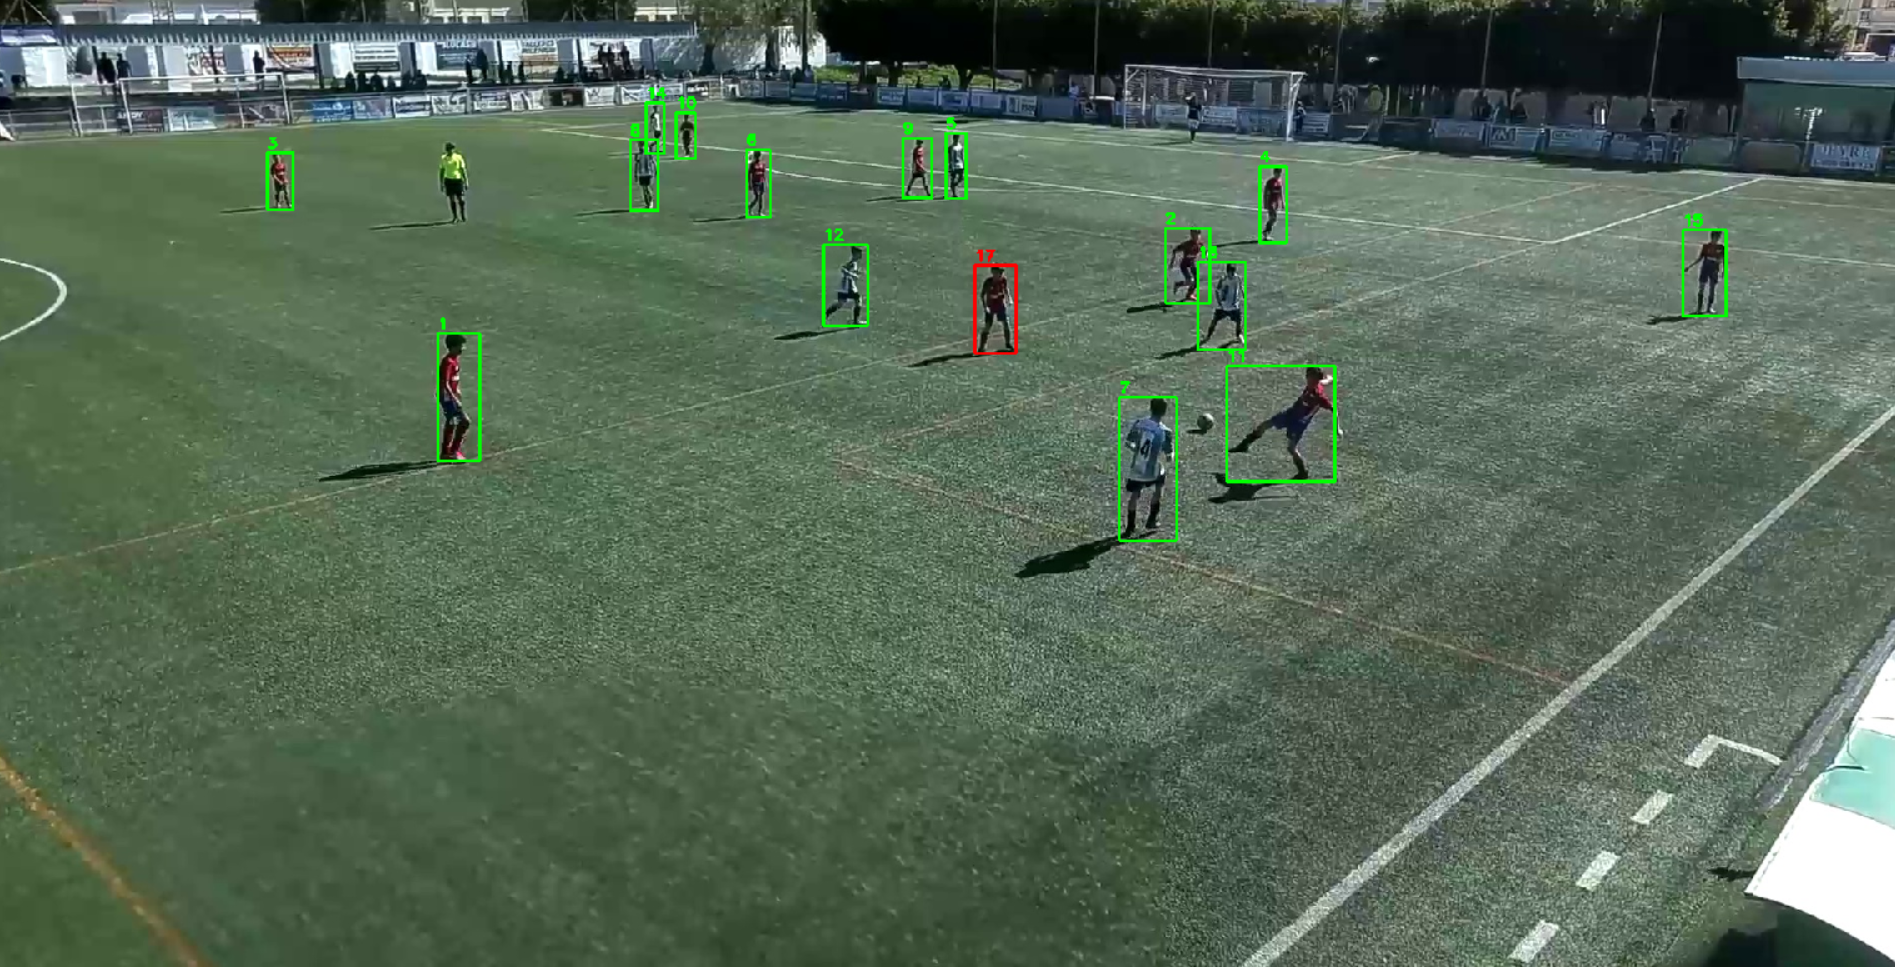
\includegraphics[width=0.8\textwidth]{image/entr_reid}
		\caption{\textbf{Programa para el entrenamiento}}
		\label{entr_reid}
	\end{figure}
	
	
	\subsubsection{annotate\_review\_precise.py}
	
	El programa \texttt{annotate\_review\_precise.py} es una versión complementaria del programa anterior \texttt{annotate\_review.py}.
	
	El código utilizado en este programa es el siguiente:
	\vspace{0.5cm}
	
	\begin{lstlisting}[style=pythonstyle]
		import os
		import cv2
		import argparse
		import tkinter as tk
		from tkinter import simpledialog
		from collections import Counter
		
		# Interactive MOT correction with manual frame control, per-frame ID modifications, approval colors, and undo
		
		def parse_mot_file(mot_path):
		entries = []
		with open(mot_path, 'r') as f:
		for line in f:
		if not line.strip(): continue
		parts = line.strip().split(',')
		entries.append({
			'frame': int(float(parts[0])),  # frame number
			'id':    int(float(parts[1])),  # original ID
			'bbox':  tuple(map(float, parts[2:6])),  # bbox
			'raw':   line.strip()  # raw line
		})
		return entries
		
		
		def draw_annotations(img, detections,
		new_ids, approved_new_ids,
		duplicate_entries, approved_dup_ids,
		raw_color_map=None, raw_index_map=None):
		out = img.copy()
		for det in detections:
		x, y, w, h = map(int, det['bbox'])
		tid = det['id']
		raw = det['raw']
		# determine color
		if raw_color_map and raw in raw_color_map:
		color = raw_color_map[raw]
		elif tid in approved_new_ids or tid in approved_dup_ids:
		color = (0, 255, 0)  # green approved
		elif tid in new_ids or any(d['id'] == tid for d in duplicate_entries):
		color = (0, 0, 255)  # red pending
		else:
		color = (0, 255, 0)
		# draw rectangle
		cv2.rectangle(out, (x, y), (x + w, y + h), color, 2)
		# prepare label
		label = str(tid)
		if raw_index_map and raw in raw_index_map:
		label += f"(i{raw_index_map[raw] + 1})"
		# put text
		cv2.putText(out, label, (x, y - 5), cv2.FONT_HERSHEY_SIMPLEX, 0.5, color, 2)
		return out
		
		
		def get_mapped_id(frame, det,
		id_map, raw_map,
		frame_id_map, frame_raw_map):
		# per-frame raw map
		if frame in frame_raw_map and det['raw'] in frame_raw_map[frame]:
		return frame_raw_map[frame][det['raw']]
		# per-frame id map
		if frame in frame_id_map and det['id'] in frame_id_map[frame]:
		return frame_id_map[frame][det['id']]
		# fallback global maps
		return raw_map.get(det['raw'], id_map.get(det['id'], det['id']))
		
		
		def pause_loop(by_frame, frames,
		id_map, raw_map,
		frame_id_map, frame_raw_map,
		removed, frames_dir,
		new_ids, duplicate_entries,
		approved_new_ids, approved_dup_ids,
		start_i):
		i = start_i
		orig_frame = frames[i]
		# color palette for duplicates
		palette = [(255, 0, 0), (255, 255, 0), (255, 0, 255), (0, 255, 255), (128, 0, 255)]
		raw_color_map = {d['raw']: palette[idx % len(palette)] for idx, d in enumerate(duplicate_entries)}
		raw_index_map = {d['raw']: idx for idx, d in enumerate(duplicate_entries)}
		
		# display duplicate info with indices
		if duplicate_entries:
		dup_info = ', '.join(f"i{idx+1}:{d['id']}" for idx, d in enumerate(duplicate_entries))
		print(f"Duplicados en frame {orig_frame}: {dup_info}")
		elif new_ids:
		print(f"Nuevos IDs en frame {orig_frame}: {new_ids}")
		print("Navegacion: [n]/[c]=next, [p]=prev, [u]=undo, [m]=modificar, [d]=delete, [q]=quit")
		
		while True:
		f2 = frames[i]
		dets2 = [d for d in by_frame[f2] if d['raw'] not in removed]
		mapped2 = []
		for d in dets2:
		mid = get_mapped_id(f2, d, id_map, raw_map, frame_id_map, frame_raw_map)
		mapped2.append({'bbox': d['bbox'], 'id': mid, 'raw': d['raw']})
		img2 = cv2.imread(os.path.join(frames_dir, f"{f2:06d}.jpg"))
		cv2.imshow('Annotations', draw_annotations(
		img2, mapped2,
		new_ids, approved_new_ids,
		duplicate_entries, approved_dup_ids,
		raw_color_map if f2 == orig_frame else None,
		raw_index_map if f2 == orig_frame else None
		))
		
		key = cv2.waitKey(0) & 0xFF
		if key in (ord('n'), ord('c')):
		approved_new_ids.update(new_ids)
		approved_dup_ids.update(d['id'] for d in duplicate_entries)
		return min(i + 1, len(frames) - 1), False
		elif key == ord('p'):
		return max(i - 1, 0), False
		elif key == ord('u'):
		return max(i - 1, 0), True
		elif key in (ord('m'), ord('d')):
		root = tk.Tk(); root.withdraw()
		sel = simpledialog.askstring("Seleccionar deteccion", "'i'<numero> o ID:")
		root.destroy()
		if not sel: continue
		# instance-level
		if sel.startswith('i'):
		try:
		idx = int(sel[1:]) - 1
		chosen = duplicate_entries[idx]
		except:
		print("Seleccion invalida"); continue
		if key == ord('m'):
		new_id = simpledialog.askinteger("Nuevo ID", "ID para esta instancia:")
		if new_id is not None:
		frame_raw_map.setdefault(orig_frame, {})[chosen['raw']] = new_id
		print(f"Instancia raw={chosen['raw']} -> {new_id} en frame {orig_frame}")
		else:
		removed.add(chosen['raw'])
		print("Instancia eliminada")
		# global-level
		else:
		try:
		orig = int(sel)
		except:
		print("ID invalido"); continue
		if key == ord('m'):
		new = simpledialog.askinteger("Nuevo ID", f"ID {orig} -> ? en frame {orig_frame}:")
		if new is not None:
		frame_id_map.setdefault(orig_frame, {})[orig] = new
		print(f"ID {orig} -> {new} en frame {orig_frame}")
		else:
		for d in by_frame[orig_frame]:
		cur = get_mapped_id(orig_frame, d, id_map, raw_map, frame_id_map, frame_raw_map)
		if cur == orig:
		removed.add(d['raw'])
		print(f"Instancias ID {orig} eliminadas en frame {orig_frame}")
		continue
		elif key == ord('q'):
		return len(frames), False
		else:
		continue
	\end{lstlisting}
	
	Este programa introduce varias mejoras y características adicionales respecto a la versión anterior:
	
	\begin{itemize}
		\item \textbf{Deshacer cambios:} La opción de deshacer (\texttt{[u]}) permite revertir los cambios realizados en el fotograma actual, añadiendo flexibilidad al proceso de corrección.
		\item \textbf{Visualización de duplicados mejorada:} Los duplicados se visualizan con colores específicos y se puede asignar un nuevo ID o eliminarlos en función de la decisión del usuario.
		\item \textbf{Control manual:} Se cambia la manera de recorrer los frames automáticamente a manualmente. Cada vez que se apruebe un frame se pasa al siguiente.
	\end{itemize}
	
	Este enfoque permite una corrección más precisa y segura, evitando acarrear ids erróneos.
	
	\begin{figure}[H]
		\centering
		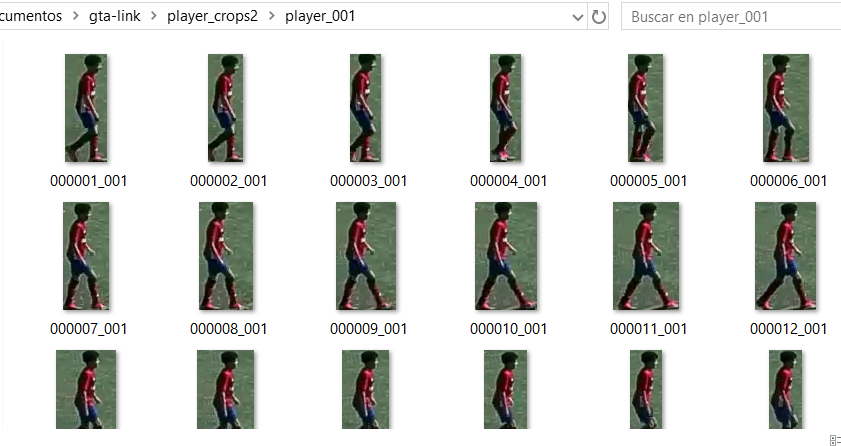
\includegraphics[width=0.8\textwidth]{image/dir_reid}
		\caption{\textbf{Estructura del dataset}}
		\label{dir_reid}
	\end{figure}
	
	\subsection{Preparar el dataset de entrenamiento del modelo de ReID}
	
	\subsubsection{dicMaker\_idPlayer.py}
	
	El programa \texttt{dicMaker\_idPlayer.py} se utiliza para procesar un archivo MOT y generar recortes de imágenes de los jugadores en cada fotograma, organizados por ID de jugador. El archivo MOT contiene las anotaciones de las detecciones para cada fotograma, y el objetivo de este programa es generar recortes individuales de cada jugador basado en esas anotaciones.
	
	El proceso se realiza en dos etapas principales:
	
	1. \textbf{Lectura y análisis del archivo MOT:} El programa lee el archivo MOT que contiene las anotaciones de cada detección (frame, ID de jugador, coordenadas de la caja delimitadora) y organiza las detecciones por fotograma.
	
	2. \textbf{Recorte y guardado de las imágenes de los jugadores:} Para cada fotograma y cada jugador identificado en las detecciones, el programa recorta la región de la imagen correspondiente a las coordenadas de la caja delimitadora y guarda cada recorte en una carpeta organizada por ID de jugador.
	
	El código utilizado en este proceso es el siguiente:
	\vspace{0.5cm}
	
	\begin{lstlisting}[style=pythonstyle]
		import os 
		import cv2
		import argparse
		from tqdm import tqdm
		
		def parse_mot_file(mot_file_path):
		detections = {}
		with open(mot_file_path, 'r') as f:
		for line in f:
		parts = line.strip().split(',')
		if len(parts) < 6:
		continue
		
		frame_id = int(float(parts[0]))
		track_id = int(float(parts[1]))
		x, y, w, h = map(float, parts[2:6])
		
		if frame_id not in detections:
		detections[frame_id] = []
		detections[frame_id].append((track_id, int(x), int(y), int(w), int(h)))
		
		return detections
		
		def crop_and_save_detections(image_folder, detections, output_folder):
		os.makedirs(output_folder, exist_ok=True)
		
		for frame_id in tqdm(sorted(detections.keys()), desc="Procesando frames"):
		img_path = os.path.join(image_folder, f"{frame_id:06d}.jpg")
		
		if not os.path.exists(img_path):
		continue
		
		img = cv2.imread(img_path)
		if img is None:
		continue
		
		for track_id, x, y, w, h in detections[frame_id]:
		track_folder = os.path.join(output_folder, f"player_{track_id:03d}")
		os.makedirs(track_folder, exist_ok=True)
		
		x1 = max(0, x)
		y1 = max(0, y)
		x2 = min(img.shape[1], x + w)
		y2 = min(img.shape[0], y + h)
		
		if x2 <= x1 or y2 <= y1:
		continue
		
		crop = img[y1:y2, x1:x2]
		
		# Cambiado el nombre del archivo al formato deseado: frameId_trackId.jpg
		output_filename = f"{frame_id:06d}_{track_id:03d}.jpg"
		output_path = os.path.join(track_folder, output_filename)
		cv2.imwrite(output_path, crop)
		
		def main():
		parser = argparse.ArgumentParser()
		parser.add_argument('--mot_file', required=True)
		parser.add_argument('--image_folder', required=True)
		parser.add_argument('--output_folder', required=True)
		
		args = parser.parse_args()
		
		print("Leyendo archivo MOT...")
		detections = parse_mot_file(args.mot_file)
		
		print("\nRecortando detecciones...")
		crop_and_save_detections(args.image_folder, detections, args.output_folder)
		
		print(f"\nProceso completado. Recortes en: {args.output_folder}")
		
		if __name__ == "__main__":
		main()
	\end{lstlisting}
	\vspace{0.5cm}
	
	El programa realiza las siguientes funciones:
	
	\begin{itemize}
		\item \textbf{Parseo del archivo MOT:} El archivo MOT se procesa para organizar las detecciones por fotograma y por jugador. Cada detección incluye las coordenadas de la caja delimitadora y el ID de jugador.
		\item \textbf{Recorte de las imágenes:} Para cada fotograma y cada jugador detectado, se recorta la imagen según las coordenadas de la caja delimitadora. Los recortes se guardan en una estructura de carpetas donde cada jugador tiene su propia carpeta identificada por su \texttt{track\_id}.
		\item \textbf{Uso de la barra de progreso:} Se utiliza la librería \texttt{tqdm} para mostrar una barra de progreso durante el procesamiento de los fotogramas, facilitando el seguimiento del proceso.
	\end{itemize}
	
	
	\subsubsection{dicMakerForTrainingReID.py}
	
	El programa \texttt{dicMakerForTrainingReID.py} se usa para reorganizar un conjunto de imágenes de jugadores en una estructura compatible con el formato Torchreid, utilizado para entrenar sistemas de Re-Identificación (ReID). El script divide las imágenes de cada jugador en tres conjuntos distintos: entrenamiento (train), consulta (query) y galería (gallery).
	
	El proceso se realiza en dos etapas principales:
	
	\textbf{Preparación de la estructura de directorios:} Crea las carpetas necesarias para los tres conjuntos de datos en el directorio de destino.
	
	\textbf{Distribución de imágenes:} Para cada jugador, divide sus imágenes disponibles en los tres conjuntos según las proporciones especificadas, asegurando un mínimo de imágenes por jugador.
	
	El código utilizado en este proceso es el siguiente:
	\vspace{0.5cm}
	
	\begin{lstlisting}[style=pythonstyle]
		import os
		import shutil
		import random
		from pathlib import Path
		
		# Parametros
		source_dir = Path(r"C:\Users\jismbs\Documents\gta-link\player_crops2")
		target_dir = Path(r"C:\Users\jismbs\Documents\gta-link\player_crops2_reid")
		
		train_ratio = 0.7
		query_ratio = 0.15
		gallery_ratio = 0.15
		
		# suman 1.0
		assert abs(train_ratio + query_ratio + gallery_ratio - 1.0) < 1e-6
		
		splits = ['train', 'query', 'gallery']
		
		for split in splits:
		(target_dir / split).mkdir(parents=True, exist_ok=True)
		
		# Para cada jugador (identidad)
		for player_folder in source_dir.iterdir():
		if not player_folder.is_dir():
		continue
		
		images = list(player_folder.glob("*.jpg"))
		if len(images) < 3:
		print(f"Saltando {player_folder.name}: no hay suficientes imagenes (minimo 3)")
		continue
		
		random.shuffle(images)
		n = len(images)
		n_train = int(n * train_ratio)
		n_query = int(n * query_ratio)
		
		split_counts = {
			'train': images[:n_train],
			'query': images[n_train:n_train + n_query],
			'gallery': images[n_train + n_query:]
		}
		
		for split, split_images in split_counts.items():
		split_target_dir = target_dir / split / player_folder.name
		split_target_dir.mkdir(parents=True, exist_ok=True)
		for img_path in split_images:
		shutil.copy(img_path, split_target_dir / img_path.name)
		
		print("Dataset reorganizado correctamente en formato Torchreid.")
		
	\end{lstlisting}
	\vspace{0.5cm}
	
	El programa realiza las siguientes funciones:
	
	\begin{itemize}
		\item \textbf{División proporcional:} Distribuye automáticamente las imágenes de cada jugador en los conjuntos train (70%), query (15%) y gallery (15%) por defecto, con validación de que la suma sea exactamente 1.0.
		\item \textbf{Filtrado de jugadores:} Omite aquellos jugadores con menos de 3 imágenes, asegurando que cada identidad tenga suficientes muestras para ser útil en ReID.
		\item \textbf{Estructura compatible con Torchreid:} Crea una organización de directorios estándar que puede ser directamente utilizada por frameworks como Torchreid.
		\item \textbf{Barrido recursivo:} Detecta automáticamente todas las carpetas de jugadores en el directorio fuente y las procesa individualmente.
	\end{itemize}
	
	\textbf{Consideraciones importantes:}
	\begin{itemize}
		\item El script mantiene la estructura original de nombres de archivos y carpetas.
		\item La distribución de imágenes es aleatoria pero determinista (depende de la semilla aleatoria de Python).
		\item Se recomienda tener al menos 3 imágenes por jugador para que la división sea efectiva.
	\end{itemize}
	
	
	
	\subsection{Entrenar los modelos de ReID con torchreid}
	
	El entrenamiento de los modelos de reidentificación se ha organizado de forma modular, siguiendo una arquitectura clara que separa las distintas responsabilidades del proceso. A continuación se describe brevemente la función de cada componente principal implicado:
	
	\begin{itemize}
		\item \textbf{datasets/sportsreid\_dataset.py}: contiene la clase del dataset personalizado utilizado para el entrenamiento. Define cómo se cargan las imágenes, las etiquetas de identidad y cómo se aplican las transformaciones necesarias.
		
		\item \textbf{engine/trainer.py}: implementa la lógica principal del entrenamiento, incluyendo el bucle de épocas, el cálculo de pérdidas, métricas y la evaluación del modelo.
		
		\item \textbf{models/model\_builder.py}: define la arquitectura del modelo de reidentificación, incluyendo la selección de backbone (por ejemplo, OSNet) y el número de clases de salida.
		
		\item \textbf{utils/transforms.py}: contiene las transformaciones de imagen aplicadas durante el preprocesamiento, tanto en fase de entrenamiento como de validación.
		
		\item \textbf{utils/visualization.py}: módulo auxiliar para visualizar imágenes junto con sus etiquetas o embeddings, útil para depuración y análisis cualitativo del modelo.
		
		\item \textbf{main.py}: archivo principal desde el que se lanza el entrenamiento. Se encarga de la configuración general, carga de parámetros y orquestación del resto de módulos.
	\end{itemize}
	
	\subsubsection{Módulo \texttt{sportsreid\_dataset.py}}
	
	Este módulo define el conjunto de datos personalizado utilizado para entrenar el modelo de reidentificación en el dominio del fútbol amateur. Se construye sobre la clase base \texttt{ImageDataset} de \texttt{Torchreid}, lo que garantiza compatibilidad directa con el resto de herramientas del framework.
	
	\paragraph{Clase \texttt{SportsReIDDataset}}
	
	La clase \texttt{SportsReIDDataset} se encarga de organizar y cargar las imágenes de jugadores, almacenadas bajo una estructura de carpetas jerárquica. Dicha estructura contiene tres subdirectorios principales: \texttt{train}, \texttt{query} y \texttt{gallery}, cada uno de los cuales agrupa las imágenes correspondientes a una fase del entrenamiento o evaluación.
	
	\begin{itemize}
		\item En cada subdirectorio, las imágenes están organizadas en carpetas con nombres como \texttt{player\_<pid>}, donde \texttt{<pid>} es el identificador original del jugador.
		\item Durante la inicialización, se recorren todas las carpetas de jugadores para extraer el conjunto total de identificadores únicos (\texttt{pid\_set}).
		\item A continuación, se construye un diccionario de reindexado \texttt{pid2label}, que asigna a cada jugador un nuevo identificador continuo, empezando desde cero. Esta reindexación es esencial para el entrenamiento, ya que el modelo espera que los identificadores sean enteros consecutivos.
	\end{itemize}
	
	Cada conjunto de datos (train, query y gallery) se carga utilizando el método privado \texttt{\_load\_set}, que genera una lista de tuplas con el siguiente formato:
	
	\begin{center}
		\texttt{(ruta\_imagen, pid, camid, dsetid)}
	\end{center}
	
	\begin{itemize}
		\item \texttt{pid}: identificador del jugador reindexado.
		\item \texttt{camid}: identificador de la cámara. Se asignan valores fijos por conjunto:
		\begin{itemize}
			\item 0 para \texttt{query},
			\item 1 para \texttt{gallery},
			\item 2 para \texttt{train}.
		\end{itemize}
		\item \texttt{dsetid}: identificador del dataset. En este caso se fija a 0 para todas las imágenes, ya que solo se usa un único conjunto de datos.
	\end{itemize}
	
	Además, si alguno de los subconjuntos se encuentra vacío, se incluye una imagen de relleno ficticia para asegurar la compatibilidad con \texttt{Torchreid}, evitando errores durante el entrenamiento.
	
	\paragraph{Función \texttt{register\_dataset}}
	
	Finalmente, se proporciona una función auxiliar \texttt{register\_dataset}, que registra el dataset personalizado bajo el nombre \texttt{sportsreid} dentro del entorno de \texttt{Torchreid}. Esto permite que se pueda referenciar directamente en los scripts de entrenamiento utilizando dicho identificador.
	
	
	\subsubsection{Módulo \texttt{trainer.py}}
	
	El módulo \texttt{trainer.py} encapsula la lógica principal para entrenar el modelo de reidentificación utilizando las herramientas provistas por el framework \texttt{Torchreid}. Este archivo define dos funciones clave: una para preparar los datos y otra para lanzar el entrenamiento.
	
	\paragraph{Función \texttt{get\_datamanager}}
	
	Esta función construye un objeto \texttt{ImageDataManager}, que se encarga de la gestión de los datos durante todo el proceso de entrenamiento y evaluación. El \texttt{DataManager} cumple un papel fundamental al encargarse de:
	
	\begin{itemize}
		\item Cargar el conjunto de datos desde el directorio especificado mediante el parámetro \texttt{dataset\_dir}.
		\item Aplicar transformaciones de preprocesamiento como volteo aleatorio (\texttt{random\_flip}) y modificación de color (\texttt{color\_jitter}).
		\item Normalizar las imágenes con la media y desviación estándar estándar de ImageNet.
		\item Organizar los datos en minibatches para entrenamiento (\texttt{batch\_size\_train=32}) y evaluación (\texttt{batch\_size\_test=100}).
	\end{itemize}
	
	El dataset utilizado está registrado bajo el nombre \texttt{sportsreid}, que corresponde al conjunto personalizado definido en el archivo \texttt{sportsreid\_dataset.py}. La resolución de las imágenes se fija a 256 píxeles de alto y 128 píxeles de ancho, dimensiones estándar para modelos de reidentificación.
	
	\paragraph{Función \texttt{train\_model}}
	
	Esta función recibe un objeto \texttt{DataManager} y un modelo previamente construido, y lanza el proceso completo de entrenamiento. Su funcionamiento se desglosa de la siguiente manera:
	
	\begin{enumerate}
		\item Se construye un optimizador utilizando el algoritmo \texttt{Adam} con una tasa de aprendizaje de 0.0003.
		
		\item A continuación, se define una política de aprendizaje basada en un plan de reducción del learning rate cada 20 épocas (\texttt{stepsize=20}), utilizando el scheduler \texttt{single\_step}.
		
		\item Se crea un objeto \texttt{ImageSoftmaxEngine}, que implementa el motor de entrenamiento y evaluación supervisada mediante entropía cruzada con suavizado de etiquetas (\texttt{label\_smooth=True}).
		
		\item Finalmente, se lanza el entrenamiento mediante el método \texttt{run}, indicando:
		\begin{itemize}
			\item La carpeta donde se guardarán los resultados y modelos entrenados (\texttt{save\_dir='log/osnet\_sportsreid'}).
			\item El número máximo de épocas (\texttt{max\_epoch=1} en esta versión inicial de prueba).
			\item Frecuencia de evaluación (\texttt{eval\_freq=-1}, lo que desactiva la evaluación intermedia).
			\item Frecuencia de impresión por consola (\texttt{print\_freq=10}).
			\item Parámetros opcionales como \texttt{test\_only=False} y \texttt{visrank=False}, que desactivan el testeo aislado y la visualización de rankings de imágenes similares.
		\end{itemize}
	\end{enumerate}
	
	Una vez finalizado el entrenamiento, se devuelve el objeto \texttt{engine}, que contiene el modelo ya entrenado y permite realizar evaluaciones posteriores.
	
	\subsubsection{Módulo \texttt{model\_builder.py}}
	
	Este módulo está dedicado a la construcción del modelo de reidentificación que se entrenará con los datos previamente preparados. Utiliza directamente las funcionalidades del framework \texttt{Torchreid}, que proporciona implementaciones de arquitecturas avanzadas diseñadas específicamente para tareas de person re-identification.
	
	\paragraph{Función \texttt{build\_model}}
	
	La función \texttt{build\_model} construye una instancia del modelo OSNet, concretamente la variante \texttt{osnet\_x1\_0}, que ha demostrado ser especialmente efectiva en tareas de reidentificación por su capacidad de capturar información multiescala y contextos locales y globales simultáneamente.
	
	El modelo se construye con los siguientes parámetros:
	
	\begin{itemize}
		\item \texttt{name='osnet\_x1\_0'}: se selecciona la arquitectura OSNet en su versión base (x1.0), entrenada originalmente sobre ImageNet.
		\item \texttt{num\_classes=num\_classes}: especifica el número de clases (identidades únicas de jugadores) que debe predecir el modelo. Este valor se determina dinámicamente en función del dataset.
		\item \texttt{loss='softmax'}: se indica que el modelo se entrenará con una función de pérdida basada en entropía cruzada estándar, compatible con clasificación supervisada.
		\item \texttt{pretrained=True}: se carga el modelo con pesos preentrenados, lo que proporciona una base más robusta que acelera la convergencia y mejora la precisión.
		\item \texttt{use\_gpu=True}: habilita el uso de la GPU para el entrenamiento, si está disponible.
	\end{itemize}
	
	La función retorna el modelo ya configurado, listo para ser entrenado con el \texttt{engine} definido en el archivo \texttt{trainer.py}. Esta separación modular permite fácilmente cambiar la arquitectura o parámetros del modelo sin alterar el resto del pipeline.
	
	
	\subsubsection{Módulo \texttt{transforms.py}}
	
	El módulo \texttt{transforms.py} define el conjunto de transformaciones de preprocesamiento que se aplican a las imágenes antes de ser introducidas al modelo de reidentificación. Estas transformaciones aseguran una representación coherente y normalizada de los datos de entrada, lo que facilita un entrenamiento más estable y eficiente.
	
	\paragraph{Función \texttt{get\_transform}}
	
	La función \texttt{get\_transform} retorna una secuencia de transformaciones encadenadas mediante \texttt{torchvision.transforms.Compose}. Las transformaciones aplicadas son las siguientes:
	
	\begin{itemize}
		\item \texttt{T.Resize((256, 128))}: redimensiona todas las imágenes a una resolución fija de 256 píxeles de alto y 128 píxeles de ancho. Esta dimensión es estándar en tareas de reidentificación, ya que mantiene la proporción corporal y reduce el coste computacional.
		
		\item \texttt{T.ToTensor()}: convierte la imagen de formato \texttt{PIL} o \texttt{numpy array} a un tensor de PyTorch, con valores normalizados en el rango [0, 1].
		
		\item \texttt{T.Normalize(mean, std)}: aplica una normalización canal a canal utilizando la media y desviación estándar de las imágenes de ImageNet:
		\begin{itemize}
			\item \texttt{mean = [0.485, 0.456, 0.406]}
			\item \texttt{std = [0.229, 0.224, 0.225]}
		\end{itemize}
		Esta normalización es fundamental cuando se emplean modelos preentrenados sobre ImageNet, como OSNet, ya que asegura una coherencia estadística entre los datos originales y los nuevos datos de entrada.
	\end{itemize}
	
	Este conjunto de transformaciones se utiliza principalmente durante la fase de inferencia o validación, ya que no incluye modificaciones aleatorias como rotaciones o cambios de color, las cuales sí se añaden durante el entrenamiento desde el propio \texttt{ImageDataManager}.
	
	\subsubsection{Módulo \texttt{visualization.py}}
	
	El módulo \texttt{visualization.py} tiene como propósito evaluar el rendimiento del modelo de reidentificación entrenado y generar visualizaciones de los resultados obtenidos. Esto resulta especialmente útil para realizar un análisis cualitativo del comportamiento del modelo, más allá de las métricas numéricas tradicionales.
	
	\paragraph{Función \texttt{visualize\_results}}
	
	Esta función realiza los siguientes pasos secuenciales:
	
	\begin{enumerate}
		\item Se carga el modelo previamente entrenado desde la ruta indicada en \texttt{model\_path}. Para ello, se instancia un modelo OSNet con un número ficticio de clases igual a 1, ya que no se requiere reentrenar el modelo. Posteriormente, se restauran los pesos entrenados mediante \texttt{load\_state\_dict}.
		
		\item Se prepara nuevamente el conjunto de datos mediante el \texttt{DataManager}, llamando a la función \texttt{get\_datamanager}, para asegurar que los datos de prueba estén correctamente cargados.
		
		\item Se realiza la extracción de características (\textit{feature extraction}) de todas las imágenes tanto del conjunto \texttt{query} como del conjunto \texttt{gallery}. Esto se hace con la función \texttt{torchreid.utils.feature\_extraction}, que retorna una matriz de distancias (\texttt{distmat}) y las listas de identidades y cámaras asociadas a cada imagen.
		
		\item Con la matriz de distancias y las identidades extraídas, se evalúan las métricas estándar en reidentificación:
		\begin{itemize}
			\item \textbf{mAP (mean Average Precision)}: evalúa la precisión media considerando el ranking completo.
			\item \textbf{CMC (Cumulative Matching Characteristics)}: calcula la tasa de aciertos en las primeras posiciones del ranking, destacando especialmente el \texttt{top-1} y el \texttt{top-5}.
		\end{itemize}
		
		\item Finalmente, se genera una visualización de los resultados mediante la función \texttt{visualize\_rank}. Esta función guarda imágenes en las que se muestran, para cada imagen de consulta, sus cinco resultados más similares en la galería. El resultado se almacena en la carpeta \texttt{visrank\_results}, facilitando una inspección visual de la calidad del ranking realizado por el modelo.
	\end{enumerate}
	
	
	\subsubsection{Módulo \texttt{main.py}}
	
	Actúa como el punto de entrada principal del sistema de entrenamiento, cuyo objetivo es el de coordinar la ejecución de todas las fases, desde la preparación de los datos hasta el entrenamiento y guardado del modelo final. Además, tiene otros bloques de verificación que ayudan a comprobar que el conjunto de datos ha sido correctamente cargado y formateado.
	
	\paragraph{Función \texttt{main}}
	
	La función \texttt{main} se compone de varios pasos organizados de forma secuencial:
	
	\begin{enumerate}
		\item \textbf{Registro del dataset personalizado.}  
		Se llama a la función \texttt{register\_dataset()} para registrar el conjunto \texttt{sportsreid} en el sistema de \texttt{Torchreid}. Esto permite que el dataset sea identificado por su nombre durante el proceso de entrenamiento.
		
		\item \textbf{Configuración de rutas.}  
		Se define la ruta al directorio raíz del dataset, que contiene las carpetas \texttt{train}, \texttt{query} y \texttt{gallery}, y también la ruta de guardado de los resultados y modelos (\texttt{save\_dir}).
		
		\item \textbf{Verificación del dataset.}  
		A modo de comprobación manual, se instancia el dataset utilizando la clase \texttt{SportsReIDDataset} y se imprimen algunos ejemplos de cada subconjunto. Esto asegura que la estructura de carpetas es correcta y que los datos han sido cargados correctamente.
		
		\item \textbf{Inicialización del gestor de datos.}  
		Se crea el \texttt{ImageDataManager} llamando a la función \texttt{get\_datamanager}, lo que permite aplicar las transformaciones y gestionar los minibatches para entrenamiento y validación.
		
		\item \textbf{Construcción del modelo.}  
		Se construye un modelo de ReID (p. ej. OSNet) con el número de clases igual al número de identidades únicas en el conjunto de entrenamiento (\texttt{num\_train\_pids}), utilizando la función \texttt{build\_model}.
		
		\item \textbf{Entrenamiento del modelo.}  
		Se lanza el entrenamiento completo mediante la función \texttt{train\_model}, que entrena el modelo sobre el conjunto de datos preparado, utilizando las configuraciones por defecto.
		
		\item \textbf{Guardado del modelo.}  
		Una vez finalizado el entrenamiento, se guarda el estado de los pesos del modelo en el archivo \texttt{osnet\_sportsreid.pth}, que puede reutilizarse posteriormente para inferencia o evaluación.
		
		\item \textbf{(Opcional) Evaluación final.}  
		Aunque está comentado en esta versión, el código incluye una llamada a \texttt{engine.test()} para realizar una evaluación final automatizada del modelo una vez entrenado.
	\end{enumerate}
	
	\paragraph{Bloque de ejecución condicional}
	
	El archivo finaliza con el típico bloque de protección:
	
	\begin{verbatim}
		if __name__ == '__main__':
		main()
	\end{verbatim}
	
	Esto asegura que la función \texttt{main()} solo se ejecute si el script se ejecuta directamente, y no cuando se importe desde otro módulo.
	
	
	
	\subsection{Preparar el dataset de testeo del modelo de ReID}
	
	Tal como se ha mencionado anteriormente, se ha preparado una serie de datos estructurados de una forma concreta en tres particiones como son train, query y gallery. Todos los recortes de imagen pertenecen a un mismo clip de vídeo de fútbol amateur, el cual se ha procesado previamente para extraer los jugadores detectados en todos los fotogramas.
	
	El conjunto train ha sido usado para el proceso de entrenamiento del modelo (OSNet en este caso) mientras que las particiones correspondientes a la evaluación son las query y gallery. Cada imagen de la query representa una instancia a buscar y se compara con todas las imágenes de la gallery, siendo este conjunto la base de búsqueda. Las imágenes de ambos subconjuntos están seleccionadas de tal forma que pertenecen a las mismas identidades que aparecen en el entrenamiento pero en distintos momentos de la secuencia del vídeo o en otras condiciones visuales.
	
	
	
	
	
	
	
	
	\section{Resultados}
	
	\subsection{Definiciones de las métricas usadas}
	
	En esta subsección definiré el significado de las métricas usadas y su importancia en la evaluación.
	
	\subsubsection{Rank-k Accuracy (Rank-1, Rank-5, Rank-10, etc.)}
	
	La Rank-k accuracy es una métrica que permite calcular con qué frecuencia la identidad correcta aparece dentro de las k predicciones más próximas (medidas mediante distancia de embeddings) generadas por el modelo considerando k: la Rank-1 accuracy mide si la identidad correcta ocupa la primera posición (top-1) cuando el modelo devuleve una predicción; ejemplos para Rank-1: para una determinada imagen de consulta (query) del jugador "player\_005", el modelo genera un embedding para la query, que confronta con todos los embeddings de la galería, con los que genera ranking ordenando los resultados (según similitud o distancia Euclídea/coseno) obteniendo el ranking. La imagen que ocupa el primer lugar (top-1) en la galería será un acierto en Rank-1, si corresponde a la misma identidad que el jugador de la query.
	
	\begin{equation}
		\text{Rank-1} = \left( \frac{\text{\# queries con identidad correcta en top-1}}{\text{\# total de queries}} \right) \times 100\%
	\end{equation}
	
	\textbf{Nota importante}: Un embbeding es transformar una imagen (por ejemplo, de un jugador) en un vector numérico, de dimensión fija (por ejemplo, 512 dimensiones), que resume su contenido visual de forma discriminativa (permite distinguir entre diferentes identidades de forma efectiva).
	
	\subsubsection{mAP – mean Average Precision}
	
	La mAP no solo toma en cuenta que la predicción correcta esté entre las top-k, sino que también se interesa por el orden de las predicciones y por cómo se distribuyen las identidades que son correctas a lo largo del ranking.
	
	Es una métrica más exigente y también más representativa de la calidad de recuperación en general.
	
	
	Para cada query:
	
	
	Se calcula el Average Precision (AP), que evalúa la precisión acumulada mientras se van encontrando imágenes correctas en el ranking.
	
	
	Finalmente, se hace la media de estos valores sobre todas las queries, que es el mean Average Precision (mAP).
	
	
	Fórmula del AP para una query con varias coincidencias relevantes:
	
	\begin{equation}
		AP = \sum_{k=1}^N P(k) \cdot \Delta r(k)
	\end{equation}
	
	Donde:
	
	\begin{itemize}
		\item $P(k)$ es la precisión en la posición $k$.
		\item $\Delta r(k)$ es el cambio en recall en esa posición.
	\end{itemize}
	
	Si solo hay una coincidencia relevante (una imagen en la galería con la misma identidad), el AP será igual a la precisión en la posición en que aparece esa coincidencia.
	
	\begin{equation}
		mAP = \frac{1}{Q} \sum_{i=1}^{Q} AP_i
	\end{equation}
	
	Donde:
	
	\begin{itemize}
		\item $Q$ es el número de queries.
		\item $AP_i$ es la \textit{average precision} para la query $i$.
	\end{itemize}
	
 	\subsection{Método de evaluación de re-identificación para YOLOv10} \cite{7410490}
 	
 	En contraste con los modelos que tienen un propósito explícito en la tarea de reidentificación de personas (ReID), como podría ser el caso del OSNet, los modelos de la familia YOLO, de los que se hace eco el mencionado modelo YOLOv10 en este trabajo, no tienen una finalidad explícita de extraer embeddings de la identidad visual de una persona, sino que se limitan a la detección de objetos en una imagen o en un vídeo, devolviendo coordenadas espaciales de las detecciones y puntuaciones de confianza y, en algunas implementaciones, los identificadores temporales que permite hacer seguimiento de la trayectoria de las detecciones, pero no tienen la capacidad de generar una descripción profunda y discriminativa de la apariencia de los objetos que detectan, de forma que tampoco se pueden aplicar para ReID.
 	
 	Para solventar esta limitación y evaluar la capacidad de YOLOv10, al menos de modo aproximado, para realizar reidentificación se propuso una alternativa que hacía uso de la simulación de un extractor de características. La solución propuesta fue la de capturar todos los recortes de personas detectados a partir de cada uno de los fotogramas del vídeo en cuestión, normalizarlos y hacer que fueran procesados a través de un módulo denominado DummyReID. Este módulo no hace uso de una arquitectura entrenada, sino que aplica una operación de media espacial global en cada uno de los tres canales de color (rojo, verde y azul) del recorte de la persona. De modo que, de esta forma, cada imagen queda convertida en un vector de tres dimensiones que resume su apariencia en cuanto a colores.
 	
 	Estos vectores, a pesar de ser muy básicos y no tener capacidad semántica alguna, permiten la aplicación de métricas clásicas de evaluación en ReID como son el Rank-k y el mean Average Precision (mAP) mediante el cálculo de distancias entre embeddings; de esta forma, por un lado, se estima qué tipo de información útil ofrece YOLOv10 en términos de identidad visual y, por otro lado, se establece una línea base (baseline) contra la cual compararemos los resultados obtenidos con modelos que sí son especialistas en ReID, como OSNet.
 	
 	
 	\subsubsection{Ejemplo de evaluación de re-identificación para YOLO}
 	
 	Supongamos que ya tenemos dos ficheros de entrada:
 	
 	\medskip
 	\noindent
 	\textbf{feats\_all.npy} con 6 embeddings (cada uno es un vector, pero aquí sólo indicamos su índice):
 	\begin{center}
 		\begin{tabular}{c|cccccc}
 			idx:   & 0 & 1 & 2 & 3 & 4 & 5 \\ \hline
 			feats: & $e_0$ & $e_1$ & $e_2$ & $e_3$ & $e_4$ & $e_5$
 		\end{tabular}
 	\end{center}
 	
 	\medskip
 	\noindent
 	\textbf{ids\_all.npy} con los IDs correspondientes:
 	\begin{center}
 		\begin{tabular}{c|cccccc}
 			idx: & 0 & 1 & 2 & 3 & 4 & 5 \\ \hline
 			ids: & 1 & 2 & 1 & 2 & 3 & 3
 		\end{tabular}
 	\end{center}
 	
 	\bigskip
 	
 	\begin{enumerate}
 		\item \textbf{Split consulta vs.\ galería.}\\
 		Para cada ID que aparece al menos dos veces:
 		\begin{itemize}
 			\item ID 1 en índices 0 y 2: consulta $q_0=0$, galería $g_0=2$.
 			\item ID 2 en índices 1 y 3: consulta $q_1=1$, galería $g_1=3$.
 			\item ID 3 en índices 4 y 5: consulta $q_2=4$, galería $g_2=5$.
 		\end{itemize}
 		Quedan consultas $[0,1,4]$ y galería $[2,3,5]$.
 		
 		\item \textbf{Matriz de distancias (Query × Galería).}\\
 		Supongamos estas distancias euclídeas:
 		\begin{center}
 			\begin{tabular}{c|ccc}
 				& $g=2$ & $g=3$ & $g=5$ \\ \hline
 				$q=0$ & 0.5 & 1.2 & 2.0 \\
 				$q=1$ & 1.0 & 0.4 & 1.5 \\
 				$q=4$ & 2.5 & 2.0 & 0.3
 			\end{tabular}
 		\end{center}
 		
 		\item \textbf{Rank-1 (mini-ejemplo).}\\
 		Para cada consulta, el candidato más cercano:
 		\begin{itemize}
 			\item $q=0$ (ID 1): mejor es $g=2$ (ID 1) → acierto.
 			\item $q=1$ (ID 2): mejor es $g=3$ (ID 2) → acierto.
 			\item $q=4$ (ID 3): mejor es $g=5$ (ID 3) → acierto.
 		\end{itemize}
 		Rank-1 = $3/3 = 100\%$.
 		
 		\item \textbf{mAP (Average Precision).}\\
 		Para cada consulta marcamos hits en el ranking completo:
 		\[
 		\begin{array}{l|c}
 			Consulta & AP \\ \hline
 			q=0 & 1.0 \\
 			q=1 & 1.0 \\
 			q=4 & 1.0
 		\end{array}
 		\]
 		\[
 		\mathrm{mAP} = \frac{1.0 + 1.0 + 1.0}{3} = 100\%.
 		\]
 		
 		En un caso real con miles de embeddings y detecciones, el procedimiento es idéntico: 
 		se calculan Rank-1, Rank-5, Rank-10 y mAP sobre las listas ordenadas de distancias.
 	\end{enumerate}
 	
 	\subsection{Evaluación de re-identificación para modelos de torchreid}
 	
 	El archivo que se ejecuta para evaluar de forma cuantitativa el rendimiento de un modelo de reidentificación previamente entrenado con imágenes del conjunto query contra el conjunto gallery es eval.py. La ejecución del script, permite obtener métricas como mAP (mean Average Precision) y Rank-k, que sirven para determinar el rendimiento de un modelo. Seguidamente se describe el funcionamiento del script a través de bloques:
 	
 	En primer lugar, se importa el módulo de la librería torchreid, que es una librería para hacer la reidentificación de personas, junto con el registro del dataset personalizado que se ha definido anteriormente en el archivo sportsreid\_dataset.py; este registro permite a torchreid reconocer y construir adecuadamente las carpetas del conjunto de datos que se tiene que separar en train, query y gallery.
 	
 	Seguidamente, se instancia un objeto de clase de tipo ImageDataManager, el que se encargará de cargar, transformar y organizar los datos. En este caso se tiene que cargar la ruta hacia el dataset, el tamaño final al que se redimensionan las imagenes(256x128 px), el tamaño de lote tanto para entrenamiento como para evaluación, y finalmente se añade una transformación de aumento de datos de tipo random\_flip (inversión horizontal aleatoria); aunque el presente script no entrene el modelo esto garantiza coherencia en el preprocesado a realizar durante la evaluación. En este punto se establece también la activación del uso de la GPU para acelerar los cálculos a realizar.
 	
 	A continuación se construye el modelo de reidentificación que se quiere evaluar, en este caso resnet50\_fc512, un modelo de ResNet50 diseñado para devolver embeddings de 512 dimensiones. Se establece el número de clases num\_classes en correspondencia al número de identidades distintas en el conjunto de entrenamiento y se decide no cargar un modelo genérico preentrenado, sino utilizar los pesos particulares que han sido obtenidos de un entrenamiento anterior. Los pesos se cargarán del archivo model.resnet50.pth.tar-20 mediante la función load\_pretrained\_weights().
 	
 	\begin{lstlisting}[style=pythonstyle]
 		import torchreid
 		from datasets.sportsreid_dataset import register_dataset
 		
 		def main():
 		# Registra el dataset
 		register_dataset()
 		
 		# Carga datos
 		datamanager = torchreid.data.ImageDataManager(
 		root='C:/Users/Soriano/OneDrive/Documentos/entrenamientoReID/player_crops2_reid',
 		sources='sportsreid',
 		height=256,
 		width=128,
 		batch_size_train=32,
 		batch_size_test=100,
 		transforms=['random_flip'],
 		use_gpu=True
 		)
 		
 		# Carga modelo y pesos
 		model = torchreid.models.build_model(
 		name='resnet50_fc512',
 		num_classes=datamanager.num_train_pids,
 		loss='softmax',
 		pretrained=False
 		)
 		
 		torchreid.utils.load_pretrained_weights(
 		model,
 		r'C:\Users\Soriano\OneDrive\Documentos\entrenamientoReID\reid_checkpoints\model.resnet50.pth.tar-20'
 		)
 		
 		# Crear el motor y lanzar evaluacion
 		engine = torchreid.engine.ImageSoftmaxEngine(
 		datamanager,
 		model,
 		optimizer=None  # Solo evaluamos, no entrenamos
 		)
 		
 		engine.test()
 		
 		if __name__ == '__main__':
 		main()
 		
 	\end{lstlisting}
 	
 	\subsection{Resultados de la evaluación de re-identificación}
 	
 	Los resultados recopilados pertenecen a los modelos de Reid aplicados al conjunto de datos etiquetado, considerando solo las detecciones de cada jugador. 
 	
 	\subsubsection{YOLOv10}
 	
 	Para YOLOv10 he tenido que hacer una evaluación más creativa para calcular las métricas.
 	
 	\begin{figure}[H]
 		\centering
 		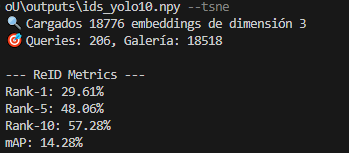
\includegraphics[width=0.8\textwidth]{image/metricas_reid_yolo10}
 		\caption{\textbf{Resultado ReID Yolov10}}
 		\label{fig:Resultado Yolov10 reid}
 	\end{figure}
 	
 	Este experimento ilustra una forma poco habitual de aproximarse a utilizar un detector como el YOLOv10 para tareas de reidentificación y el resultado lo deja claramente manifiesto para tal propósito.
 	El YOLOv10 está especializado para tareas de detección, no para reconocer si las clases son (muy) similares visualmente. Su arquitectura es capaz de localizar objetos, no de mapear imágenes en el espacio donde las distancias reflejan similitud de identidad, además de que sus capas de salida están especificamente diseñadas para boxes delimitadores, no para embeddings.
 	El resultado lo pone de manifiesto: un Rank-1 que solamente alcanza el 29.6% y un muy bajo mAP del 14.28%; esto significa que el modelo no puede identificar correctamente la mayoría de los jugadores ni siquiera para los 5 o 10 primeros candidatos. Por ello, el método de ReID que se pretende implantar es aplicable a un sistema de ReID con modificaciones extremas.
 	
 	
 	\subsubsection{Osnet Sportsmot}
 	
 	\begin{figure}[H]
 		\centering
 		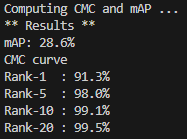
\includegraphics[width=0.8\textwidth]{image/sports_model.pth.tar-60_sportsmot}
 		\caption{\textbf{Resultado ReID con Osnet entrenado con el dataset de Sportmot}}
 		\label{fig:Resultado DeepEIoU con Osnet reid sportsmot osnet_x1_0}
 	\end{figure}
 	
 	Este modelo, que se basa en OSNet, fue entrenado con el dataset SportsMOT, un dataset de fútbol profesional que contiene secuencias de jugadores en entornos controlados y de alta calidad visual. La arquitectura OSNet permite extraer de manera efectiva tanto la información visual global como local, lo que se traduce en su alta Rank-1 del 91.3%. Sin embargo, el mAP solo es del 28.6%, lo que implica que mientras el modelo tiende a clasificar correctamente la imagen, el resto, las imágenes relacionadas con la misma identidad, no están clasificadas correctamente; esto es consistente con el hecho de que el modelo fue entrenado sobre un deporte profesional pero no se adapta a las características propias del fútbol amateur: cámaras distantes, resoluciones más bajas, variaciones de luz, recortes menos precisos. En resumen, el rendimiento sugiere que el modelo responde de manera adecuada con los ejemplos más evidentes, pero no es capaz de conseguir agrupar las distintas apariciones de un mismo jugador.
 	
 	A pesar de que es un modelo OSNet entrenado específicamente en el dominio futbolístico, las diferencias que existen del dominio en un sentido profesional y amateur limitan la capacidad de generalizar, lo que afecta la calidad general de la escala y penaliza el mAP.
 	

  	
 	\subsubsection{Osnet Soccernet}
 	\begin{figure}[H]
 		\centering
 		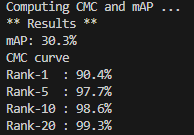
\includegraphics[width=0.8\textwidth]{image/model.osnet.pth.tar-10_soccernet}
 		\caption{\textbf{Resultado ReID con Osnet entrenado con el dataset de Soccernet}}
 		\label{fig:Resultado DeepEIoU con Osnet reid soccernet osnet_x1_0}
 	\end{figure}
 	
 	El presente modelo también se basa en OSNet, aunque, a diferencia del anterior, no se encuentra ajustado al dominio, sino que cuenta con preentrenamiento realizado sobre SoccerNet, es decir, un dataset profesional de fútbol.
 	
 	El hecho de que el atributo Rank-1 sea relativamente alto (90.4%) pero el valor mAP sólo llegue al 30.3% es indicativo de que en los casos en que el modelo acierta, estos son los más evidentes, pero en el caso de ejemplos ambiguos, el performance decay es grande, lo cual tiene todo el sentido dado que SoccerNet suele contener imágenes de mejor calidad (múltiples cámaras bien calibradas, contexto mejor regulado), mientras que tu dataset normalmente contiene imágenes en situaciones de mayor ruido visual, con compresión, aficiones visuales de pose o escales. 
 	Un modelo tiene la capacidad de identificar patrones generales (forma del cuerpo, color de la camiseta) pero no está ajustado para poder lidiar con las especificidades visuales del fútbol amateur, lo que se traduce en un deterioro muy importante en las predicciones que son más difíciles.
 	
 	El hecho de que OSNet sea una arquitectura potente sólo nos puede llevar a la conclusión que el desajuste de dominio impide la precisión global del modelo.
 	
 	\subsubsection{ResNet Soccernet}
 	\begin{figure}[H]
 		\centering
 		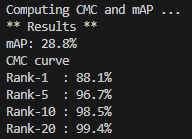
\includegraphics[width=0.8\textwidth]{image/model.resnet50.pth.tar-20_soccernet}
 		\caption{\textbf{Resultado ReID con Resnet entrenado con el dataset de Soccernet}}
 		\label{fig:Resultado  con Resnet reid soccernet resnet50_fc512}
 	\end{figure}
 	
 	A pesar de las ventajas que proporciona su arquitectura, que es clásica y robusta, ResNet-50 no es una arquitectura adecuada para ReID por sí sola, ya que se enfoca en la extracción de características muy globales, abstractas, sin un mantenimiento local de la información espiritual. Mientras que OSNet es una arquitectura desenvolvente que extrae características de varias escalas y es capaz de mantener la información al nivel local, ResNet-50 tiende a extraer características más globales (aunque también reciben información de las escalas restantes).
 	Esto perjudica el rendimiento en tareas como la reidentificación de las personas, donde los detalles visuales estereotipados marcan la gran diferencia. Al final, el resultado es similar al modelo OSNet preentrenado, pero un poco inferior, en especial en Rank-1.
 	
 	A pesar de ser robusta, ResNet-50 pierde poder de discriminación frente a las arquitecturas entrenadas de manera específica a la tarea (OSNet) y su rendimiento hace evidentes estas capacidades.
 	
 	\subsubsection{Osnet mi dataset estiquetado}
 	\begin{figure}[H]
 		\centering
 		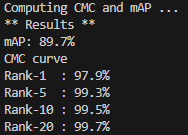
\includegraphics[width=0.8\textwidth]{image/resultado_entrenamiento_reid_myData_osnet}
 		\caption{\textbf{Resultado ReID con Osnet entrenado con mi dataset etiquetado}}
 		\label{fig:Resultado  con Osnet reid mi dataset etiquetado osnet_x1_0}
 	\end{figure}
 	
 	El máximo rendimiento de toda la batería de pruebas corresponde a este modelo, porque es el modelo mejor adaptado a la problemática de clasificar el fútbol amateur, dado que está entrenado directamente sobre las imágenes de tu propio conjunto de datos.
 	OSNet está diseñado para aprender características discriminativas a la vez que captura información a nivel local y global gracias a su diseño multi-escala y a sus bloques convolucionales eficientes. En fotografía de fútbol amateur (donde las condiciones de luz, resolución y calidad son muy variables), esta arquitectura es particularmente adecuada en cuanto a que puede sacarle el mejor provecho a elementos visuales muy finos (textura de las camisetas, siluetas, posturas, etc.) para distinguir a los jugadores.
 	
 	Una mAP alta indica que el modelo es capaz de mantener la consistencia incluso en los casos más difíciles, y un Rank-1 cercano al 98% indica que en la mayoría de las consultas el primer candidato es correcto.
 	
 	\subsection{Resultados de MOT}
	
	\begin{figure}[H]
		\centering
		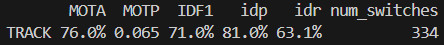
\includegraphics[width=0.8\textwidth]{image/metricas_mot_yolo10}
		\caption{\textbf{Resultado MOT Yolov10}}
		\label{fig:Resultado Yolov10 mot}
	\end{figure}
	
	\begin{figure}[H]
		\centering
		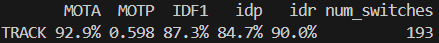
\includegraphics[width=0.8\textwidth]{image/metricas_mot_deepEIoU_osnet_sportmot}
		\caption{\textbf{Resultado MOT DeepEIoU con Osnet entrenado con el dataset de Sportmot}}
		\label{fig:Resultado DeepEIoU con Osnet mot sportmot}
	\end{figure}
	
	\begin{figure}[H]
		\centering
		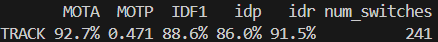
\includegraphics[width=0.8\textwidth]{image/metricas_mot_deepEIoU_osnet_soccernet}
		\caption{\textbf{Resultado MOT DeepEIoU con Osnet entrenado con el dataset de Soccernet}}
		\label{fig:Resultado DeepEIoU con Osnet mot soccernet}
	\end{figure}
	
	resnet50\_fc512
	
	
	\section{Cosas adicionales que hice}
	
	\subsection{Entrenar un modelo de YOLOv8 con un dataset etiquetado propio}
	
	https://roboflow.com/
	
	Para entrenar el modelo de detección de jugadores, utilizamos la plataforma Roboflow, una herramienta online ampliamente utilizada para gestionar datasets de visión por computador. Roboflow facilita la carga, etiquetado, preprocesado y exportación de conjuntos de datos en formatos compatibles con múltiples frameworks de deep learning, incluyendo YOLO.
	
	En nuestro caso, el proceso comenzó con la recopilación de fotogramas extraídos de vídeos de partidos de fútbol amateur. Estos frames fueron subidos a Roboflow, donde se realizó el etiquetado manual de los jugadores. Cada jugador fue anotado mediante la creación de una \textit{bounding box} alrededor de su figura, y se le asignó la clase \texttt{jugador}.
	
	Aunque en este proyecto únicamente se ha utilizado una clase (\texttt{jugador}), Roboflow permite una gestión flexible de múltiples clases. En el caso de que se hubiera querido incluir también la detección de otros roles como \texttt{árbitro} o \texttt{balón}, bastaría con asignar un nuevo nombre de clase a las anotaciones correspondientes durante el etiquetado. Cada vez que se etiqueta un objeto en un fotograma, se puede seleccionar (o crear) la clase deseada desde el menú desplegable de etiquetas.
	
	
	\begin{figure}[H]
		\centering
		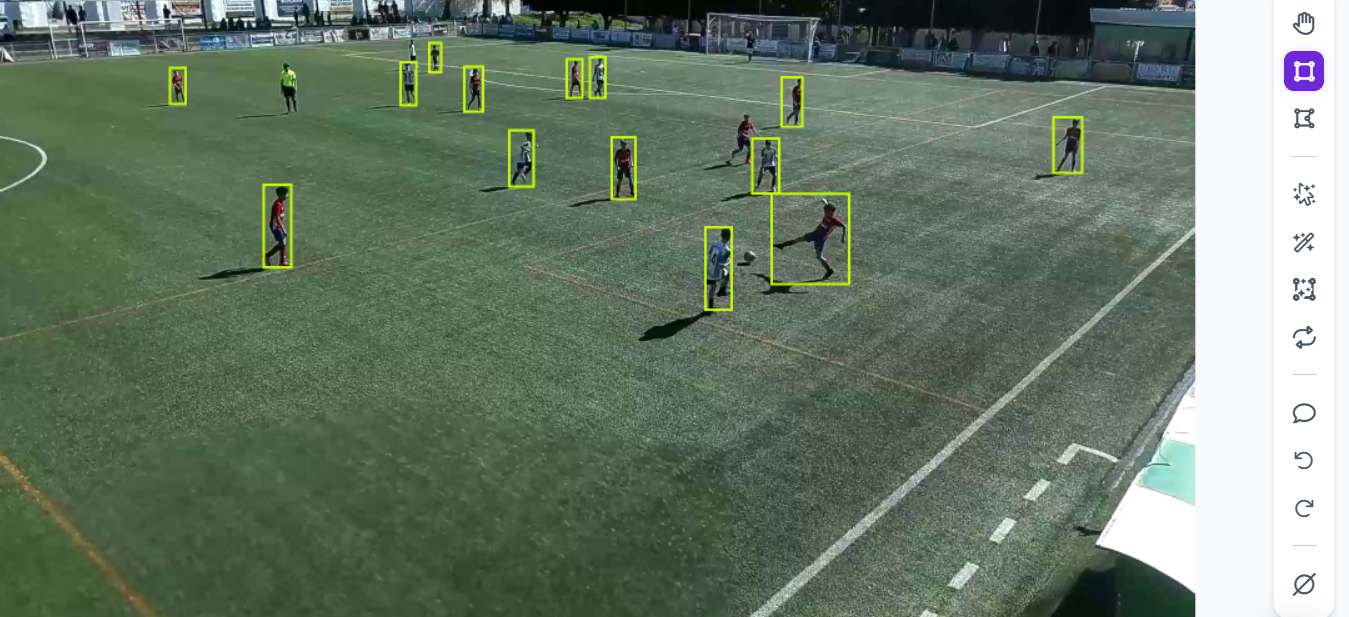
\includegraphics[width=0.8\textwidth]{image/dif_de_clases}
		\caption{\textbf{Diferenciación de clases}}
		\label{dif_de_clases}
	\end{figure}
	
	De este modo, el dataset resultante puede incluir múltiples clases, y el modelo YOLO aprenderá a diferenciarlas durante el entrenamiento, basándose en sus apariencias y posiciones relativas. Esta capacidad de distinguir entre diferentes tipos de objetos resulta esencial en contextos deportivos donde intervienen múltiples agentes.
	
	\begin{figure}[H]
		\centering
		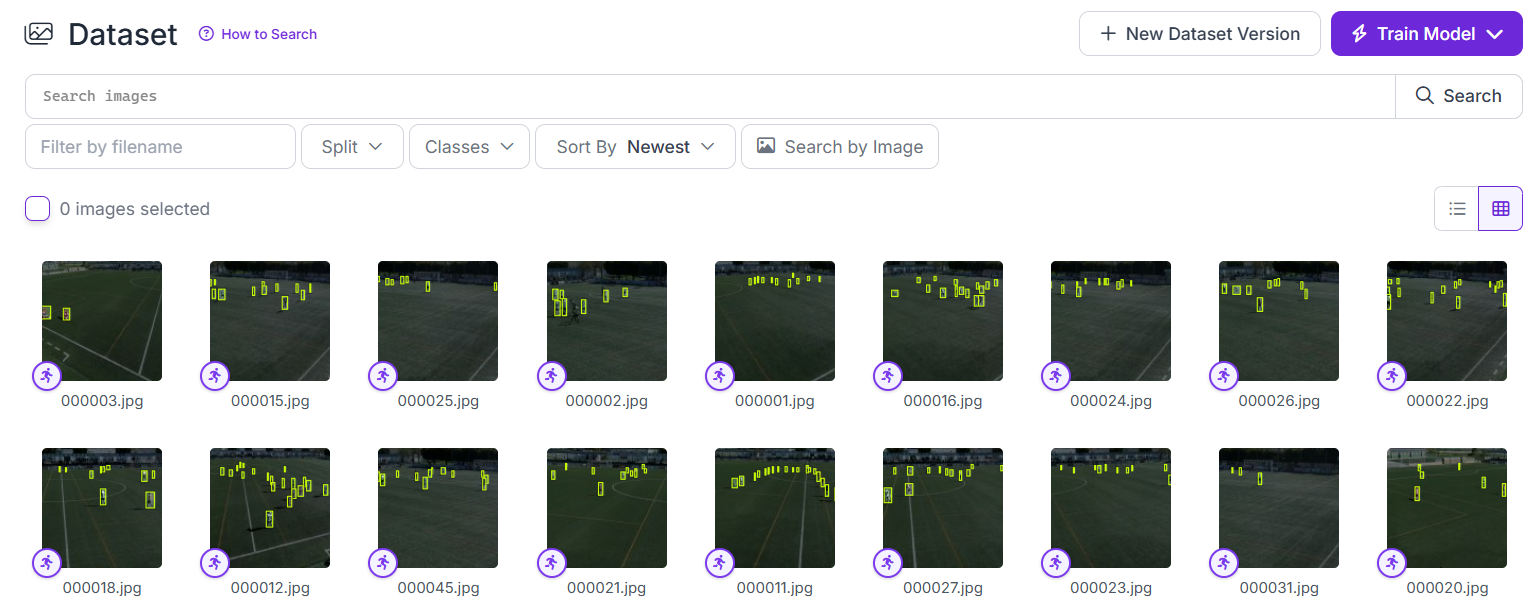
\includegraphics[width=0.8\textwidth]{image/entr_yolo}
		\caption{\textbf{Entrenamiento YOLO}}
		\label{entr_yolo}
	\end{figure}
	
	Una vez completado el etiquetado, el dataset fue exportado desde Roboflow en el formato YOLOv5/YOLOv8, incluyendo las anotaciones en archivos de texto por imagen, y un archivo \texttt{data.yaml} que especifica la configuración general del conjunto de datos, como las rutas, el número de clases y sus nombres.
	
	
	\subsection{Entrenamiento del modelo de YOLO}
	
	Una vez preparado el conjunto de datos en Roboflow y exportado en formato compatible con YOLOv8, se procedió al entrenamiento del modelo utilizando el framework \texttt{Ultralytics}, que proporciona una implementación optimizada y fácil de usar de los modelos YOLO.
	
	El entrenamiento se realizó en Python, comenzando por la descarga del dataset directamente desde la API de Roboflow. Para ello, se utilizó el siguiente fragmento de código:
	
	\begin{verbatim}
		from roboflow import Roboflow
		rf = Roboflow(api_key="sONwHlD0Zcp6DurtT8Nw")
		project = rf.workspace("pruebabalonmano").project("handball-dataset-def-2")
		version = project.version(1)
		dataset = version.download("yolov8")
	\end{verbatim}
	
	Este código descarga automáticamente las imágenes y las anotaciones en formato YOLOv8, incluyendo el archivo \texttt{data.yaml} con la configuración del dataset.
	
	A continuación, se cargó un modelo base preentrenado \texttt{yolov8n.pt} (versión ligera del modelo), y se inició el entrenamiento personalizado con los parámetros definidos:
	
	\begin{verbatim}
		from ultralytics import YOLO
		
		model = YOLO("yolov8n.pt")  # Modelo base preentrenado
		results = model.train(
		data=f"{dataset.location}/data.yaml",
		epochs=25,
		imgsz=640,
		batch=16,
		name="yolov8_handball"
		)
	\end{verbatim}
	
	En este caso, se entrenó durante 25 épocas, con imágenes de tamaño 640×640 píxeles y un tamaño de lote (\texttt{batch size}) de 16 imágenes. El modelo aprende a identificar la clase \texttt{jugador} a partir de los ejemplos anotados.
	
	Una vez finalizado el entrenamiento, se genera automáticamente el archivo \texttt{best.pt}, que contiene los pesos del modelo con mejor rendimiento en validación. Este modelo final puede utilizarse directamente para la inferencia:
	
	\begin{verbatim}
		best_model = YOLO("runs/detect/yolov8_handball/weights/best.pt")
	\end{verbatim}
	
	Este flujo de trabajo permite adaptar el modelo YOLOv8 a un dominio concreto, como el fútbol amateur, utilizando anotaciones específicas y obteniendo así un detector más ajustado al contexto real de aplicación.
	
	
	\section{Dificultades encontradas}
	
	
	
	\section{Conclusiones}
	
	
	
	%%%%%%%%%%%%%%%%%%%%%%%%%%%%%%%%%%%%%%%%%%%%%%%%%%%%%%%%%%%%%%%%%%%%%%%%%%%
	\printbibliography
	
	
	%% Back Cover
	
\includepdf[noautoscale=true, width=\paperwidth]{backcover.pdf}
	
\end{document}